

\documentclass[letterpaper,12pt]{book}

%
%  Build command:
% pdflatex -shell-escape  CtlBook.tex
%
% (-shell-escape option is required for minted code listing highlighting)
% Uncomment for bibliog.
%\bibliographystyle{unsrt}
\usepackage{amsmath}
\usepackage{amssymb}
\usepackage{boxedminipage}
\usepackage{caption}
\usepackage{color}
\usepackage{enumitem}
\usepackage{fancyhdr}
\usepackage[T1]{fontenc}
\usepackage{framed}
\usepackage{graphicx}
\usepackage{hyperref}
\usepackage{listings}
\usepackage{mdframed}
\usepackage{tcolorbox}
\usepackage{xcolor}

% tikz package for block diagrams
\usepackage{tikz}
\usetikzlibrary{arrows,calc,patterns,decorations.pathmorphing,decorations.markings}
\tikzset{>=latex} % blockier style arrow heads


\newcommand{\grad}{\bigtriangledown}
\newcommand{\pd}{\partial}
\newcommand{\br}{\epsilon \mathcal{R}}

% --
% HOMEWORK Page headers
% %%%%%%%%%%%%%%%%%%%%%%%%%%%%% HEADER / FOOTER
% \pagestyle{fancy}
% %%%%%  Page header/footer fields for "NSF Style" proposal
% %%%%%  \chead will be changed with each section
% \pagestyle{fancy}
% \lhead{\small\sc ECE233}
% <h>\chead{\large\bf Homework 4}
% <n>\chead{\large\bf Homework 4 {\bf SOLUTIONS}}
% \rhead{ver: \today}
% \lfoot{Hannaford, U. of Washington}
% \rfoot{Aut. 2025}
% \cfoot{\thepage}
%
% --

\pagestyle{fancy}
\lhead{Chapter \thechapter}
%\chead{CENTER HEADER}
\rhead{\today}
\lfoot{ECE233, U. of Washington}
%\rfoot{\today}
\rfoot{\thepage}
%%%%%%%%%%%%%%%%%%%%%%%%%%%%%%%%%%%%%%%%%%%%%%%%
%
%  Set Up Margins

%%%%%%%%%%%%%%%%%%%%%%%%%%%%%%%%%%%%%%%%%%%%%%%%%
% include file for:
%      Critical Page setup dimensions
%            DO NOT MODIFY
%       (for help see "Latex Line by Line" p 260)
%
\setlength\oddsidemargin{0in}
\setlength\evensidemargin{0in}

\usepackage[left=0.98in, right=0.98in, top=1.0in, bottom=1.0in]{geometry}

% %Top Margin and header
% \setlength\voffset{-0.94in}
% \setlength\topmargin{0.25in}
% \setlength\headheight{0.25in}
% %\setlength\headwidth{6.5in}
% \setlength\headsep{0.25in}
% %Body
% \setlength\textwidth{6.5in}
% \setlength\textheight{9.50in}
% %Footer
% %\setlength\footheight{0.5in}
% \setlength\footskip{0.3750in}
% Line spacing for 6 lines per inch
\linespread{0.894}  % 1.0 = single    1.6 = double
%
%          END of Critical Page Setup Dimensions
%%%%%%%%%%%%%%%%%%%%%%%%%%%%%%%%%%%%%%%%%%%%%%%%%%%

%%%%%%%%%%%%%%%%%%%%%%%%%%%%%%%%%%%%%%%%%%%%%%%%%%%
%
% Useful style and math macros
%


\newcommand\Dfrac[2]{\frac{\displaystyle #1}{\displaystyle #2}}
\newcommand\beq{\begin{equation}}
\newcommand\eeq{\end{equation}}

\newcommand\bmat{\begin{bmatrix}}
\newcommand\emat{\end{bmatrix}}

\newenvironment{solution}
{\ttfamily \vspace{0.155in} {\bf SOLUTION:} \\ }
{ \vspace{0.25in} \par }



%%%%%%%%%%%%%%%%%%%%%%%%%%%%%%%%%%%%%%%%%%%%%%%%%%%%%%
%
%  Example environment
%
\newcounter{Example}[chapter]

\newenvironment{Example}
% begin
{\refstepcounter{Example}\newpage
 \begin{boxedminipage}{\textwidth} % \linenumbers
    {\bf Example \thechapter.\theExample}\\
}
% end
{\vspace{0.1in}\end{boxedminipage}
\vspace{0.4in} }

\newenvironment{ExampleCont}
% begin
{
 \begin{boxedminipage}{\textwidth}\linenumbers
    {\bf Example \thechapter.\theExample \hspace{4pt} cont.}\\
}
% end
{\vspace{0.1in}\end{boxedminipage}
\vspace{0.4in} }


\newenvironment{ExampleSmall}
% begin
{\refstepcounter{Example}
\vspace{0.2in}
 \begin{boxedminipage}{\textwidth}
    {\bf Example \thechapter.\theExample}\\
}
% end
{\vspace{0.05in}\end{boxedminipage}
\vspace{0.25in} }
%
%%%%%%%%%%%%%%%%%%%%%%%%%%%%%%%%%%%%%%%%%%%%%%%%%%%%%


%%%%%%%%%%%%%%%%%%%%%%%%%%%%%%%%%%%%%%%%%%%%%%%%%%%
%
%    Minted package for nice python highlighting
%
\usepackage[chapter]{minted}  % python syntax highlight

% Required packages

% Configure minted styling
\setminted[python]{
    frame=lines,
    framesep=2mm,
    baselinestretch=1.0,
    fontsize=\footnotesize,
    linenos=true,
    breaklines,
    %     style=monokai,
    style=default
}
\setminted[C]{
    frame=lines,
    framesep=2mm,
    baselinestretch=1.0,
    fontsize=\footnotesize,
    linenos=true,
    breaklines,
    %     style=monokai,
    style=default
}

% Configure listing to have a specific width
\setminted{
    numbersep=2pt,    % Distance between line numbers and code
    xleftmargin=20pt, % Left margin (increase if line numbers still overflow)
    xrightmargin=-2pt  % Right margin (decrease to reduce extra white space)
}

% Configure listing caption style
\DeclareCaptionFormat{listing}{\raggedright#1#2#3}
\captionsetup[listing]{
    format=listing,
    labelfont=bf,
    font=small,
    labelsep=period
}

%%%%%%% end of minted %%%%%%%%%%%%%%%%%%%%%%%%%%%%%%%%%%%%%%%%%%%%


%%%%%%%%%%%%%%%%%%%%%%%%%%%%%%%%%%%%%%%%%%%%%%%%%%%%%%%%%%%%%%
%       Claude formatting code begins here
\definecolor{claudeBlue}{RGB}{59, 89, 152}
\definecolor{claudeGray}{RGB}{242, 244, 248}

\newcommand{\humanquery}[1]{%
  \par\vspace{\baselineskip}%
  \noindent%
  \fbox{%
    \parbox{\dimexpr\linewidth-2\fboxsep-2\fboxrule\relax}{#1}%
  }%
  \par\vspace{\baselineskip}%
}

\newcommand{\claudereply}[1]{%
  \par\vspace{\baselineskip}%
  \noindent%
  \fcolorbox{claudeBlue}{claudeGray}{%
    \parbox{\dimexpr\linewidth-2\fboxsep-2\fboxrule\relax}{%
      \ttfamily\raggedright #1%
    }%
  }%
  \par\vspace{\baselineskip}%
}
%%%%%%%%%%%%%%%%%%%%%%%%%%%%%%% Claude formatting code ends here


%
%   quick type equation envir.
%
\def\bq{\begin{equation}}
\def\eq{\end{equation}}

% Symbol defs for equations
\def\ef{\mathcal{E}}
\def\fl{\mathcal{F}}

% Laplace Transform
\newcommand{\sL}{\mathcal{L}}



\setlength{\headheight}{15.25pt}
\addtolength{\topmargin}{-2.49998pt}

\frontmatter

\begin{document}

\title{Lecture Notes ECE 233 }

\author{Blake Hannaford}

\maketitle

\date{\today\\(C) Copyright 2025, Blake Hannaford.\\
\href{http://creativecommons.org/licenses/by-sa/4.0/}{Creative Commons Attribution-ShareAlike 4.0 International License}.}
%
\tableofcontents
%
% % \input{Preface.tex}
%
%
\mainmatter
%
% % \linenumbers

\newpage


%
\chapter{Review of Fundamentals}

\section{Complex Number Concepts required for EE233}\label{cnconcepts}
\begin{itemize}
  \item $j = \sqrt{-1}$
  \item complex number is the sum of a real part, $\sigma$ + an imaginary part $j\omega$ (where $\omega$ is a real number to be multiplied by $j$.)
  \item   The {\it magnitude} of a complex number is the Pythagorean sum of the real and imaginary parts:
  If $x= a+jb$ is a complex number, then the magnitude is
  \[
  |x| = \sqrt{a^2+b^2}
  \]
  \item To add together two complex numbers, add their real and imaginary parts separately.
  \[
  x = a+bj \qquad y = c+dj
  \]
  \[
  x + y = (a+c) + j(b+d)
  \]
  \item To multiply two complex numbers, multiply them together like two first order polynomials in $j$ (using the definitions above)
  \[
  x*y = (a+bj)*(c+dj) = ac+adj + bcj+bdj^2
  \]
  since $j^2=-1$ we have
  \[
  x*y = (ac-bd)+(ad+bc)j
  \]

  \item Complex numbers describe a point in the {\it complex plane}.  The $X$ axis of the complex plain is the real part of the complex number and the $Y$ axis is the imaginary part.

  \item To plot the point $a+jb$ on the complex plane, plot a point at $X = a, \: Y = b$.

  \item The magnitude of a complex number is the distance from the origin to its point on the complex plane.

  \item The {\it angle} of a complex number is the angle formed from the positive real axis ($X>0$) and the line between the origin and the point.

  \item There is an \href{http://en.wikipedia.org/wiki/Euler\%27s_formula}{exponential form} of any complex number:
  \[
  e^{j\theta} = \cos(\theta) + j\sin(\theta)
  \]
  \item To convert a complex number to exponential form we invert the previous equation:
  \[
  a+bj = |a+bj| e^{j\tan^{-1}(b/a)}
  \]

  \item The $\tan^{-1}()$ function traditionally limits us to quadrants I and IV of the complex plain.    More generally we can use the 4-quadrant 2-argument arctan function \href{http://en.wikipedia.org/wiki/Atan2}{({\tt atan2(b,a)}) }.

  \item A consequence of multiplication of complex numbers and the exponential represenation of complex numbers is that when we multiply two complex numbers:
     \begin{quotation} {\it ``angles add and magnitudes multiply''}
     \end{quotation}
   if $A,B,C$ are complex numbers and $C = A * B$
   \[
    \angle{C} = \angle{A}+\angle{B}  \qquad   |C| = |A|*|B|
   \]


\end{itemize}

\subsubsection{Kahn Academy Videos}\label{KahnV}

\href{https://www.khanacademy.org/math/algebra/complex-numbers/complex_numbers/v/complex-numbers}{complex numbers}

\href{https://www.khanacademy.org/math/trigonometry/imaginary_complex_precalc/complex_analysis/v/exponential-form-to-find-complex-roots}{exponential form of complex numbers}




\newpage
\section{Complex Numbers}


Complex numbers make use of the famous imaginary number
$i = \sqrt{-1}$.    In ECE that is confusing with current so we use instead
\[
  j = \sqrt{-1}
\]

An {\it imaginary} number is any real number multiplied by $j$ such as
\[
10j,\; -4j,\; 14.7j, \; \mathrm{etc.}
\]

A {\it complex} number is the sum of a real number plus an imaginary number:
\[
  Z = a + bj
\]

\subsection{Complex Plane}

We represent complex numbers in the {\it Complex Plane}.   The complex plane is
a version of the $X,Y$ plane where each complex number represents a point or vector.
The real part is the $X$ coordinate and the imaginary part is the $Y$ coordinate.

For example the two complex numbers

\[
Z_1 = 2 + 3j, \quad Z_2=-1-3j
\]
can be drawn on the complex plane below as:

[Graphic]
\vspace{3.5in}
%\includegraphics[width=0.5\textwidth]{figsChapt01/MR6732.png}

Like any plane, the complex plane can also be addressed in polar coordinate form.
Below is the relationship between the complex number components in Cartesian and
polar forms:

\vspace{0.15in}
\begin{align}
\text{Complex} &    & \text{Polar}  \\ \hline
Z &= a + bj & &= r\angle\theta \\
a &= \text{Re}\{Z\} & r &= \sqrt{a^2+b^2} & \text{Magnitude} \\
b &= \text{Im}\{Z\} & \theta &= \tan^{-1}\left(\frac{b}{a}\right) & \text{Angle}
\end{align}


\subsection{Exponential Form}

One of the most famous equations in mathematics is Euler's Identity:
\begin{equation}
\boxed{e^{j\theta} = \cos(\theta) + j\sin(\theta)}
\end{equation}

\begin{equation}
e^{j\pi} = -1
\end{equation}



\subsection{ Computation with Complex Numbers}

\noindent Rectangular Form:
\[
\text{Addition:}       \quad  (a + bj) + (c + dj) = (a+c) + (b+d)j
\]
\[
\text{Multiplication:} \quad  (a + bj) \times (c + dj) = ac + adj + bcj + bdj^2 = ac-bd + (ad+bc)j
\]

\noindent Polar Form:

\[
\text{Addition:} \quad       r_1\angle\theta_1 + r_2\angle\theta_2
\]
\[
\text{Multiplication:} \quad (r_1\angle\theta_1)\times(r_2\angle\theta_2 = r_1r_2\angle(\theta_1+\theta_2)
\]

So each operation (addition or Multiplication) is easiest in one of the two forms, summed up with the slogan
\begin{quotation}``Angles add, Magnitudes multiply''\end{quotation}

\noindent{Exponential Form}
Note that the polar form is derived from Euler's exponential form:
\begin{align}
\text{Addition:} \quad &\text{Euler's $e^{j\alpha}$} \\
\text{Multiply:} \quad &A_1e^{j\theta_1} \cdot A_2e^{j\theta_2} = A_1A_2e^{j(\theta_1+\theta_2)}
\end{align}



\subsection{Complex Conjugate}
If $Z = a + jb$ then its complex conjugate, $Z^* = a - jb $, in other words to get the Complex conjugate of  a complex
number, just multiply its imaginary part by $-1$.
If we multiply a complex number by its conjugate, it is easy to see that we get its Magnitude:

\[
ZZ^* =  (a+bj)(a-bj) = a^2 - abj + abj - b^2j^2 = a^2 + b^2
\]

[Graphic]
%\includegraphics[width=0.5\textwidth]{figsChapt01/MR6733.png}


\begin{align}
\text{e.g. Division:} \quad \frac{Z_1}{Z_2} &= \frac{a_1 + b_1j}{a_2 + b_2j} = \frac{Z_1 \cdot Z_2^*}{Z_2 \cdot Z_2^*} = \frac{Z_1Z_2^*}{|Z_2|^2}
\end{align}

\subsection*{Complex Number Arithmetic in a nutshell:}
\begin{tabular}{l|p{1.in}|p{1.0in}|p{1.0in}}
Form                 & Add           & Multiply           & Conjugate \\\hline
Rectangular, $a+bj$  & By Component  & Like a Polynomial  & Negate imaginary part\\ \hline
Polar,
$A\angle{\theta}$    & like Vectors  & Angles Add, Magnitudes Multiply & Negate Angle \\ \hline
Exponential,
$Ae^{j\theta}$       & Convert to rectangular! & just like Polar & Negate exponent
\end{tabular}

\subsection{Examples}

Q: What is $\sqrt{-64}$?

A: $\sqrt{-1 \cdot 64} = \sqrt{-1} \cdot 8 = j8$ or imaginary \#

Q: What is $2 + \sqrt{-36}$?


A: $2 + j6$, which can't be simplified, the solution is
a Complex \# that can be considered to
be two projections of a  vector.

We think of $j$ as a unit vector $90^\circ$ away from the real axis.


Therefore, their sum is the projection of their vector
sum:
\subsection{Magnitude}
$r = \sqrt{2^2 + 6^2} = \sqrt{4 + 36} = 6.32$
\subsection{Angle}
$\theta = \tan^{-1}\left(\frac{36}{4}\right) = 83.66^\circ = 1.46 \text{ rad}$

\subsection{two Complex numbers}

\[
A = 3+5j,\; B = -2-2j
\]

(the easy way):
\[
A+B = (3-2) + (5-2)j = 1+3j
\]

\subsection{the hard way }
Consider them as magnitude/angle:
\[
|A| = \sqrt{3^2+5^2} = 5.83,\; \angle{A} = \tan^{-1}(5/3) = 71.5^\circ
\]
\[
|B| = \sqrt{2^2+2^2} = 2.83,\; \angle{B} = \mathrm{atan2}(-2,-2) = 225^\circ
\]
(note can't use $\tan^{-1}$!)
Now adding is like vectors:


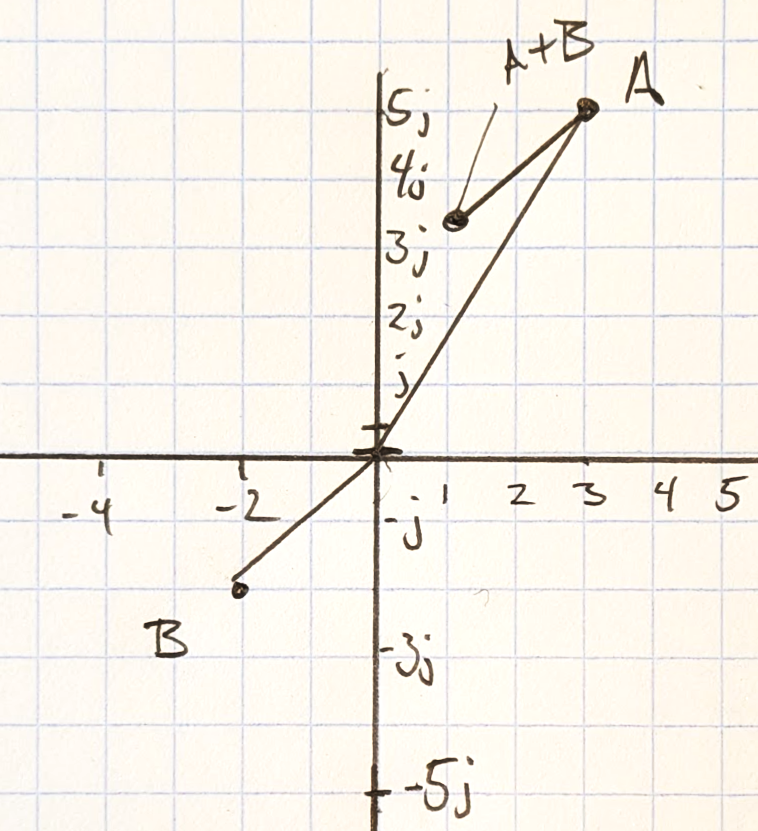
\includegraphics[width=.5\textwidth]{figsChapt01/AA65506.png}







\section{Kirchoff's Current and Voltage Laws (KCL, KVL)}

\subsection{KCL}
In our context we can express KCL as follows:

If a node connects $n$ conductors having currents, $i_1 \dots i_n$,
then
\[
\sum_k i_k = 0
\]
Physically this means that charge cannot accumulate on a node and give it a
potential (of course a capacitor {\it can} accumulate charge!).

\subsection{KVL}
Our version of KVL states:

If a circuit loop, consists of $n$ nodes (which may belong to other loops as well),
and we define the $k^{th}$ branch as the branch connecting node $k$ with node $k-1$, and if $V_k$ is defined as the voltage drop across the branch:
\[
V_k = v_k - v_{k-1}
\]
(where $v_k$ is the voltage at node $k$)
then KVL is
\[
\sum_k V_k = 0
\]
In words, the sum of the voltage drops around any loop is equal to zero. In an
every day example, if you walk any closed path around the streets of Seattle,
your net gain in elevation (net change of potential energy) must be zero.

For more complex circuits having more than one node or loop,
KCL and KVL are frequently used to generate a set of equations which can be
jointly solved to get all the node voltages or branch currents.


\subsection{KCL/KVL examples}


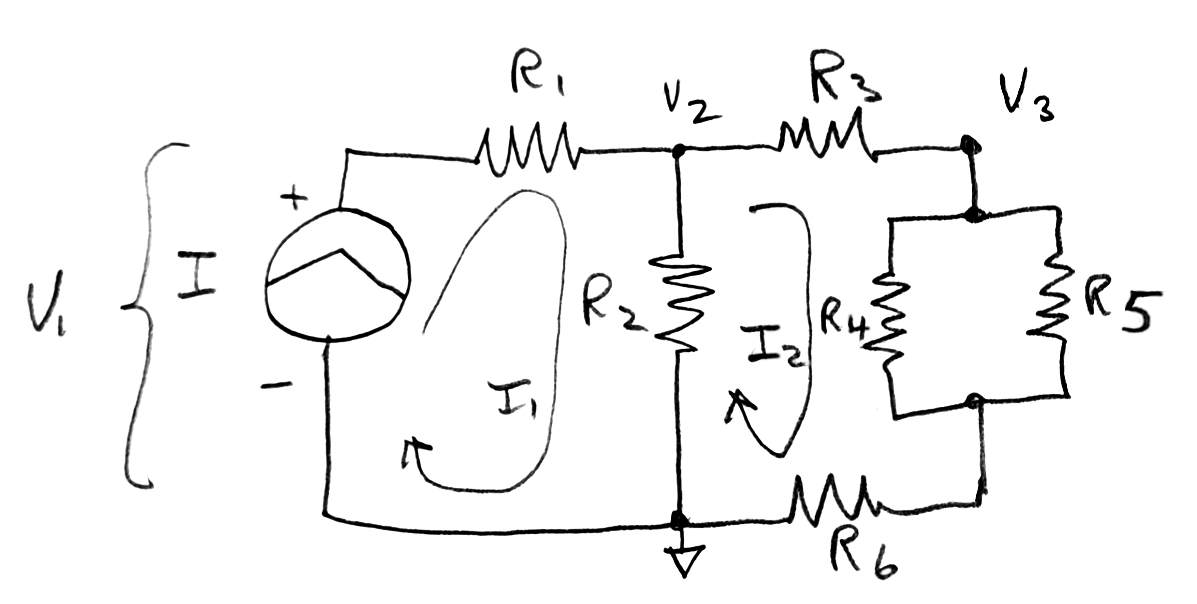
\includegraphics[width=.75\textwidth]{figsChapt01/IG95777.png}

\subsection{KVL}
 Write two KVL equations for the two loops above (|| resistors don't count as a loop!).

1)
\[
V_1+I_1R_1+(I_1+I_2)R2=0
\]

2)
\[
I_2R_3+I_2(R_4||R_5)+I_2R+6+(I_2-I_1)R_2=0
\]

\subsection{KCL}
For the same circuit, write a KCL equation for the node which joins $R_1,R_2,R_3$,  in terms
of the three node voltages:
\[
\frac{V_1-V_2}{R_1}+\frac{-V_2}{R_2} + \frac{V_3-V_2}{R_3} = 0
\]


\section{Basic Operational Amplifier Configurations}


\subsection{Inverting Amplifier}

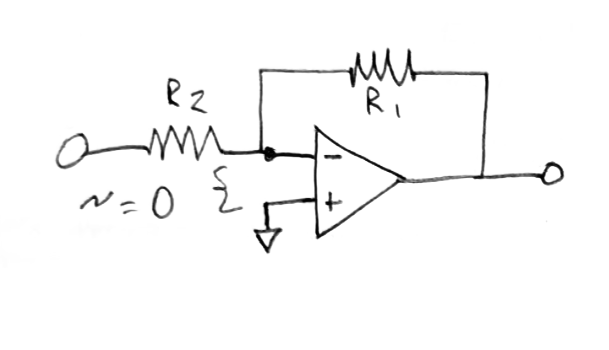
\includegraphics[width=60mm]{figsChapt01/BV83562.png}


\[
G = \frac {-R1}  {R2}
\]
\subsection{Non-inverting Amplifier}
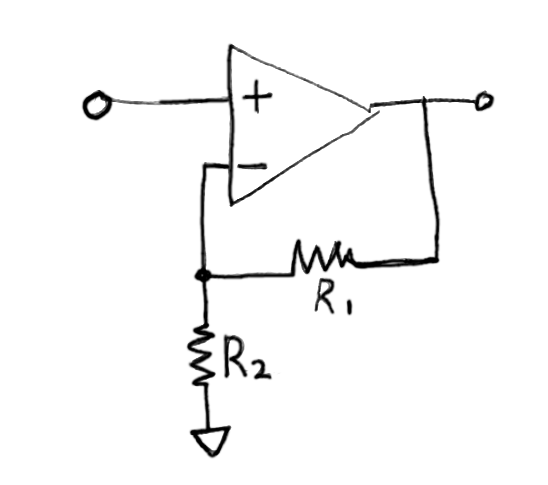
\includegraphics[width=50mm]{figsChapt01/PN49388.png}
\[
G=\frac {+R1}  {R1+R2}
\]
\subsection{Summing Amplifier}
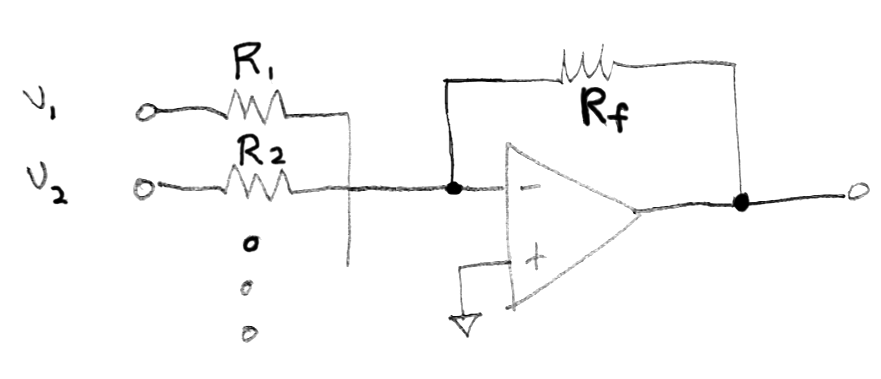
\includegraphics[width=90mm]{figsChapt01/GC91051.png}
\[
V_O= -V_i\sum_i \frac {R_f}  {R_i}
\]
\subsection{Voltage Follower}
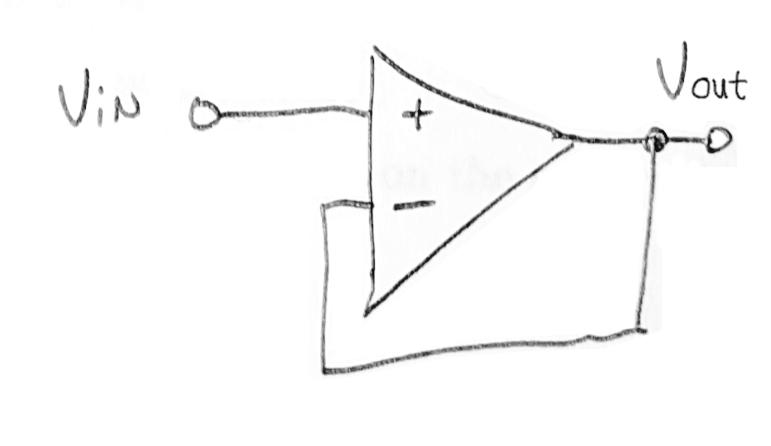
\includegraphics[width=50mm]{figsChapt01/BI19090.png}
\[
V_O = V_{in}
\]
\section{deciBells (dB)}


\subsection{Decibels}

Decibels are a logarithmic\footnote{Take the quiz and review logs if necessary: Section \ref{LogReview}} unit which are widely used for the analysis of frequency response.   If we have a quantity, $x$, then
\[
dB(x) = 20\log_{10}(x)
\]
where $dB(x)$ represents the decibel representation of $x$.


Because decibels are logarithmic units, we will make frequent use of the following properties (which are easily proved using basic properties of logarithms)

\[
dB(ab) = dB(a)+ dB(b)
\]
\[
dB(a/b) = dB(a) - dB(b)
\]
\[
dB(\sqrt{a}) = \frac {dB(a)}{2}
\]
etc.

Some handy {\it approximate} $dB$ values, when  memorized, give you very quick and accurate (within 5\%) hand calculation results:

\[
3.16 = \sqrt{10} = 10dB ,\quad 10 = 20dB, \quad 100 = 40dB
\]
\[
2 = 6dB, \quad   \sqrt{2} = 3dB
\]
\[
1/2 = -6dB, \quad \frac{1}{\sqrt{2}} = \frac{\sqrt{2}}{2} = -3dB
\]
etc.


\begin{ExampleSmall}
Convert the following quantities to $dB$.

\[
dB(1000) = 20\log(1000) = 20*3 = 60dB
\]
\[
dB(6000) = dB(1000\times6) = dB(1000) + dB(6)  = 60 + 15.6 = 76.6dB
\]
\[
dB(X/100) \quad (\mathrm{where }\quad dB(X)=40dB) = 40 - 20\log(100) = 40-40 = 0dB
\]

\end{ExampleSmall}

\section{2, and 4 quadrant arc-tangent functions}

It's easy to see that
regular arctangent is limited to quadrants I and IV!

\vspace{2.5in}
\[
tan^{-1}(\frac {-5}  {-3} ) = tan^{-1}(\frac {5}  {3} )
\]


The real word goes around the
whole circle, so we define the 4-quadrant arctan function:
\[
\mathrm{atan2}(Y,X)
\]
which figures out the right way to apply arctan() depending on the quadrants.


\section{Voltage Dividers}


\section{Series and Parallel Resistors}


\vspace{3.0in}
\section{Thevenin and Norton equivalent circuits}

\subsection{Thevenin}
\vspace{3.5in}
Thevenin Stuff

\subsection{Norton}
\vspace{3.5in}
Norton Stuff


\section{Energy Storage Elements}

\subsection{Capacitors}

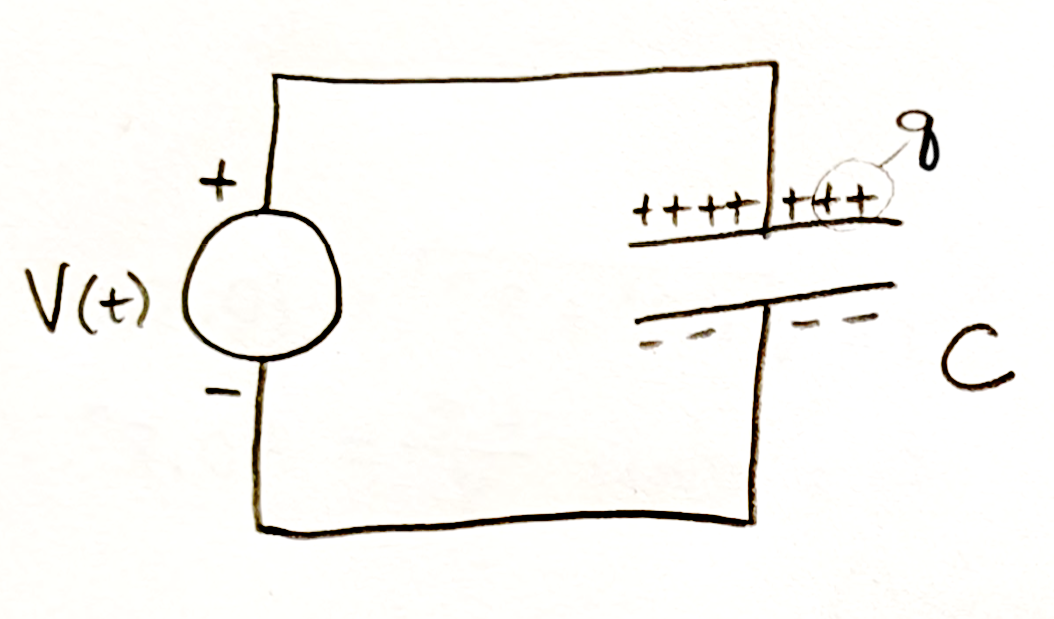
\includegraphics[width=.5\textwidth]{figsChapt01/SA77254.png}

Charge:
\[
q = CV
\]
Current
\[
i = \frac {dq}  {dt}  = C\frac {dV}  {dt}
\]
Charge
\[
q = \int_{-\infty}^t i dt =  \int_{-\infty}^t  C\frac {dV}  {dt}
\]
Voltage
\[
V = 1/C \int_{0}^t i dt+ \int_{-\infty}^0 i dt + 1/C q_{(t=0)}
\]
\[\boxed{
V=\frac {1}  {C} \int_{-\infty}^t i\; dt }
\]

Energy
\[
E_C = \int_{-\infty}^t V(t)i(t)dt = \int_{-\infty}^t VC\frac {dV}  {dt} = C\int_{-\infty}^t VdV
\]
\[
= \left . \frac {1}  {2}CV^2(t)\right | ^t_{-\infty} \;\;
\]
Finally
\[
E_C(t) = \frac {1}  {2}CV^2(t) \; \mathrm{, assume~ } V(-\infty) = 0 \;\mathrm(Joules)
\]

\subsection{Inductors}

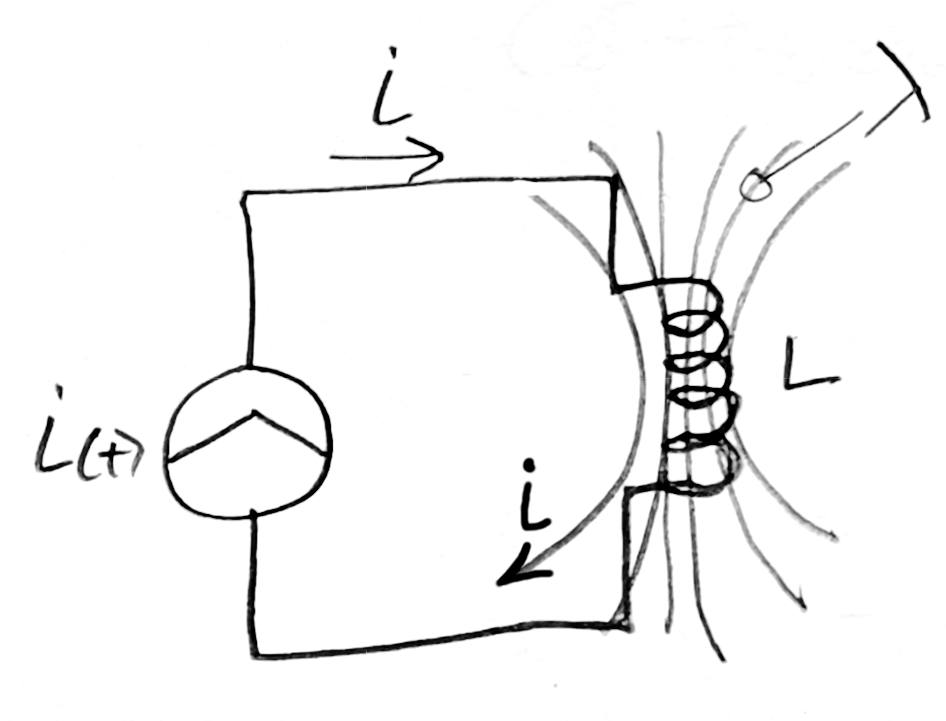
\includegraphics[width=.5\textwidth]{figsChapt01/GM98526.png}

Mag Field:
\[
\lambda = Li
\]
Voltage
\[
V = \frac {d\lambda}  {dt} = \frac {d}  {dt} Li
\]
\[\boxed{
V(t) =  L\frac {di}  {dt}   }
\]
Energy
\[
E_L = \int_{-\infty}^t V i\; dt = \int_{-\infty}^t L\frac {di}  {dt} i \;dt
\]
\[
L\int_{-\infty}^t i\; di = \frac {1}  {2} Li^2(t)  \; \mathrm{(Joules)}
\]


  % Review


\chapter{Steady State Sinusoidal Analysis}


\section{Sinusoids}

A sinusoid is a time function of the form
\[
  A \sin(\omega t + \phi)
\]
where


\vspace{0.2in}
\begin{tabular}{c|l|l}
Name    & Meaning  & Units\\\hline
$A$   &  Amplitude  &  Volts, Amps, etc \\
$\omega$   & Frequency  & $rad/sec$ \\
$t$     & Time  & $sec$  \\
$\phi$  & Phase & $rad$  \\
\end{tabular}

\vspace{0.2in}
Sinusoids arise in ECE through two primary ways
\begin{enumerate}

\item The mathematical solutions to circuits built-up of R, L, C elements sometimes
contain sinusoidal terms.

\item Rotating machines like generators primarily generate sinusoidal voltages.   Our regular wall outlets
have a sinusoidal voltage with frequency 60 Hertz, 377 rad/sec.

\end{enumerate}


Some properties of sinusoids include:

\begin{itemize}

\item Since $\omega$ is in $rad/sec$, we must frequently convert frequencies in cycles per second (Hertz)
by noting that one cycle is $2\pi$ radians. Thus for example:

  \[
    1000 Hz = 2\pi\times 1000 \approx 6283.2 rad/sec
    \]

\item The Phase angle, $\phi$, slides the sinusoid back and forth along the time axis acording to its value
(which is a constant).  There are special cases when $\phi$ is a multiple of $\pi/2$ such as
\[
  A \sin(\omega t + \pi/2) = -A \cos(\omega t)
  \]

or
\[
  A \sin(\omega t + \pi) = -A \sin(\omega t)
  \]
according to various trig identities.

\item Since $\sin()$ and $\cos()$ have important geometrical interpretations, it is not surprising that it is often useful to
visualize a sinusoid as a projection of a rotating vector onto the $X$ or $Y$ axis.

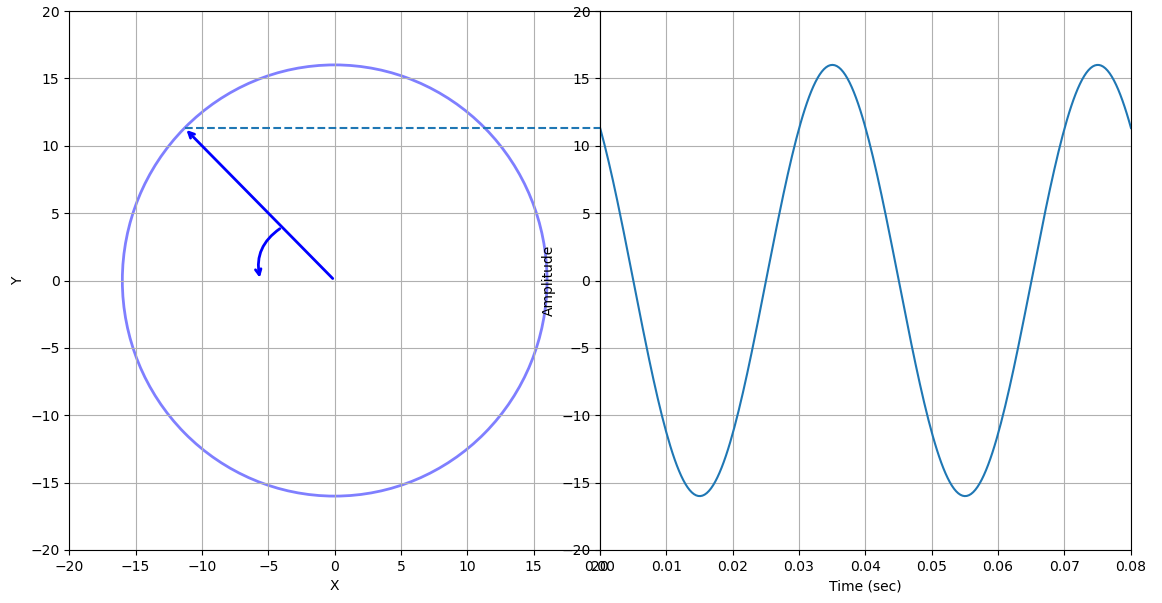
\includegraphics[width=0.5\textwidth]{figsChapt02/MQ41BN01.png}

In the left panel, a vector rotates counter-clockwise at rate $\omega$ radians
per second.   If we trace the y component of the vector over time, we get the
sinusoid appearing on the right.
\href {https://youtu.be/a_zReGTxdlQ?si=hQbJcQvjlW3IVkuE&t=73} {[Animation from Kahn Academy]}

\end{itemize}

\subsection*{Sinusoid Review Problems}

\subsubsection*{basic functions}
For the following graph,

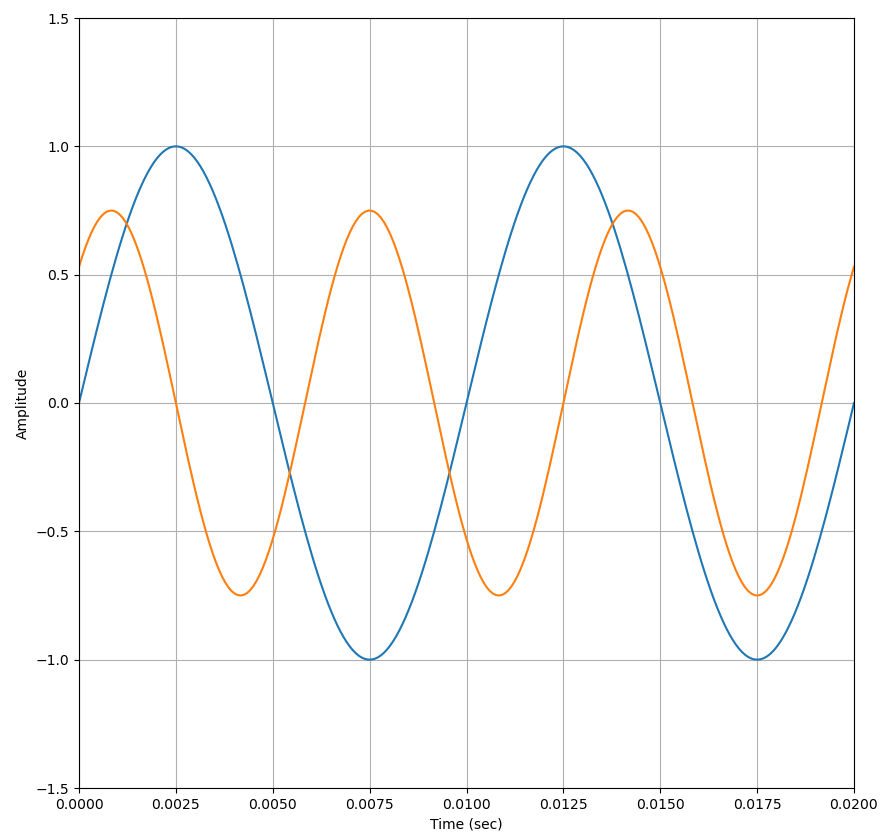
\includegraphics[width=0.5\textwidth]{figsChapt02/MQ41BN02.png}

\paragraph{Problem:}
Find the equation of the two sinusoids.

\paragraph{Solution:}

Looking at corresponding peaks or zero-crossings of the blue trace, the amplitude, $A$, is 1.0, and
the period, $P$,   is 0.01 seconds so using:

\[
P  =  2\pi/\omega_{bl}
\]
\[
  \omega_{bl} = 2\pi/0.01 = 628.3 \;rad/sec
\]

at $t=0, \sin(\omega_{bl}t + \phi_{bl}) = 0$ so $\phi_{bl} = 0$, and the equation is:
  \[
    y_b(t) = 1.0\sin(628.3t)
    \]
For the orange wave, the amplitude is 0.75 and checking the time of the 3rd and 2nd peaks
(or any 2 successive peaks):
\[
P = 0.0142 - 0.0075 = 0.0067 sec
\]

\[
  \omega_o = 2\pi/0.0067 = 937.8 \;rad/sec
\]
reading the graph,
at $t=0$, $\sin(\omega_ot + \phi_o) = 0.5$ so at $t=0$, $\sin(\phi_o) = 0.5/0.75 \; \to \; \phi_o = 0.73 rad \approx 42^\circ$,
so the equation is
\[
y_o(t) = 0.75\sin(937.8t+ 0.73)
\]



{\bf Additional Problems:}

\begin{enumerate}


\item  {\bf Problem:}
For both the orange and blue waves, find time where $\theta = \omega t+\phi =  0$ (using $\sin(0) = 0$):

{\bf Solution:}\\
    Blue: $\omega_{bl} t + \phi_{bl} = 0$ plugging in values above, we have $628.3t+0=0 \; \to\; t = 0$.\\
    Orange: $\omega_o t + \phi_o = 0$ plugging in values above, we have $937.8t+0.730=0, t = \frac{-0.730}{937.8}=-.00078$,  this value is not plotted but adding one half period gives $t=-0.00078+0.0067/2 =0.00257$


\item {\bf Problem:} Also for both waves, find time where $\theta = \pi/2$ (using $\sin(\pi/2)=1$)

  {\bf Solution:}\\
    Blue: $628.3t+0=\pi/2\;\to\;t = 0.0025$\\
    Orange: $937.8t+0.73 = \pi/2\;\to\;t=0.000897$

\item Check the above solutions by inspection of the graphs.
\end{enumerate}




\subsection{Phase Shifts }  Looking back at the blue and orange waves, We can see that there is a
phase difference between them, and we derived that it was 0.73 radians.
Recalling the equations of our two waves:
\[
y_b(t) = 1.0\sin(628.3t)
\]
\[
y_o(t) = 0.75\sin(937.8t+ 0.73)
\]
Let's consider $y_b(t)$ the ``reference'' wave.

Note that in comparing any two waves, we can set the
phase shift of one of them to zero (unless there is some additional time reference).  For example
if

\[
y_1(t) = 1.0\sin(200t - \pi)
\]
\[
y_2(t) = 0.75\sin(200t +\pi/2)
\]
The following two sinusoids have the same relationship to each other:
\[
y_1(t) = 1.0\sin(200t + 0)
\]
\[
y_2(t) = 0.75\sin(200t + 3\pi/2)
\]
(we have added $\pi$ to both arguments.)

\paragraph{Phase Lag and Phase Lead}

Definition:

\begin{quotation}
If the phase shift of wave B with respect to wave A is $\phi>0$, then
wave B {\bf leads} wave A.
\end{quotation}


Definition:

\begin{quotation}
If the phase shift of wave B with respect to wave A is $\phi<0$, then
wave B {\bf lags} wave A.
\end{quotation}


Referring back to the blue and orange waves above, the phase shift of the orange
wave compared to the blue wave is positive ($+0.73rad$) so the orange wave {\bf leads} the
blue wave.  Indeed it  peaks earlier in time than the blue wave does.



\subsection{Sum of 2 sinusoids}
\paragraph{Example:}

{\bf Problem: }
\[
V(t) = 8\cos(\omega t + \pi/3) + 4\cos(\omega t)
\]

{\bf Solution: }

Note that each sinusoid can be considered to be a projection of a rotating vector:


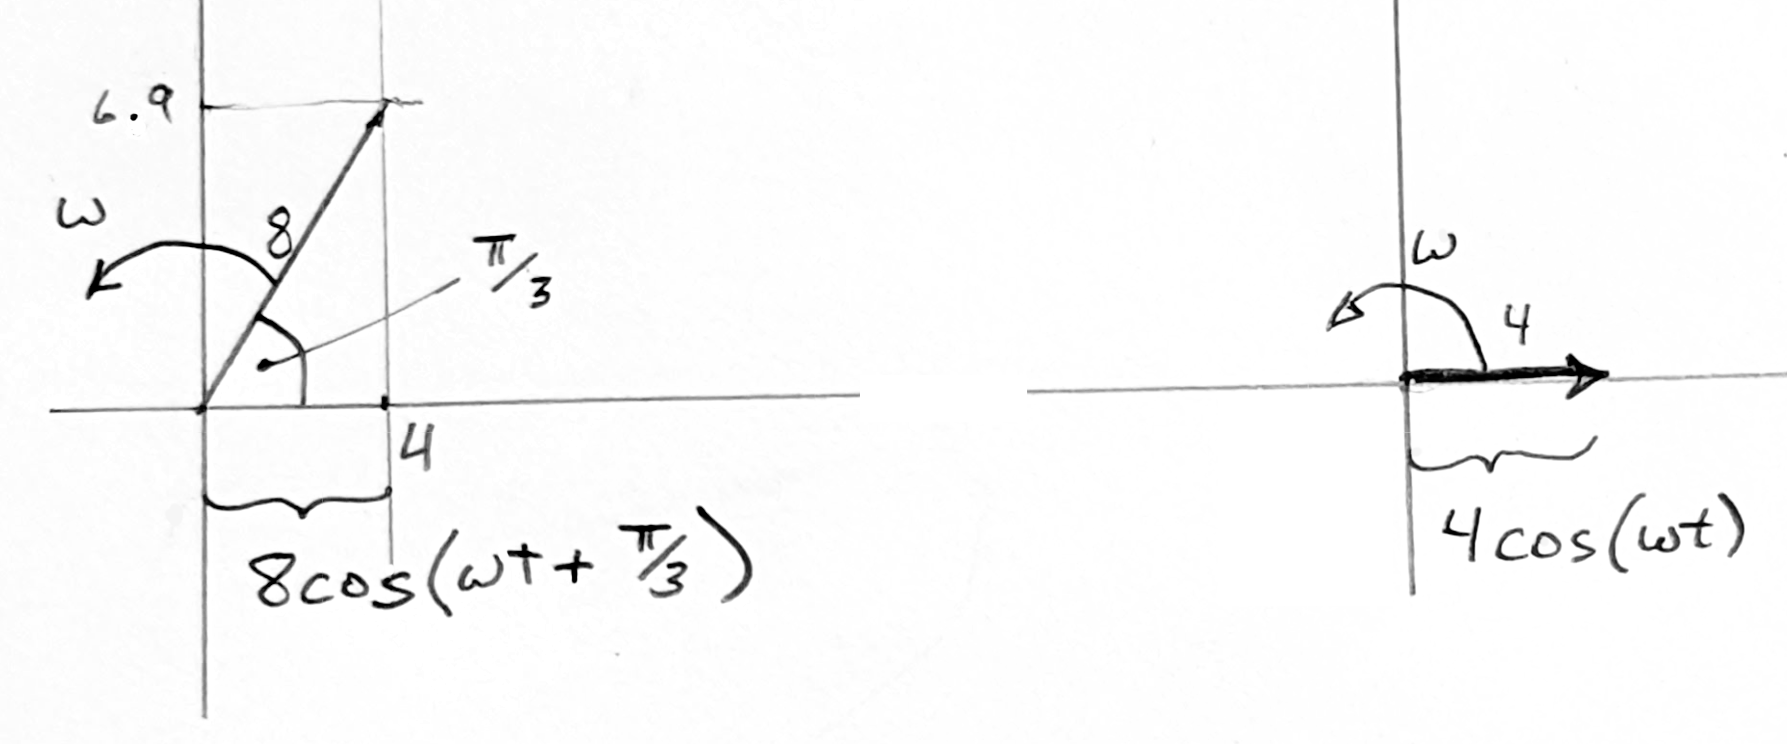
\includegraphics[width=\textwidth]{figsChapt02/KG21706.png}

Therefore, their sum is the projection of their vector sum:

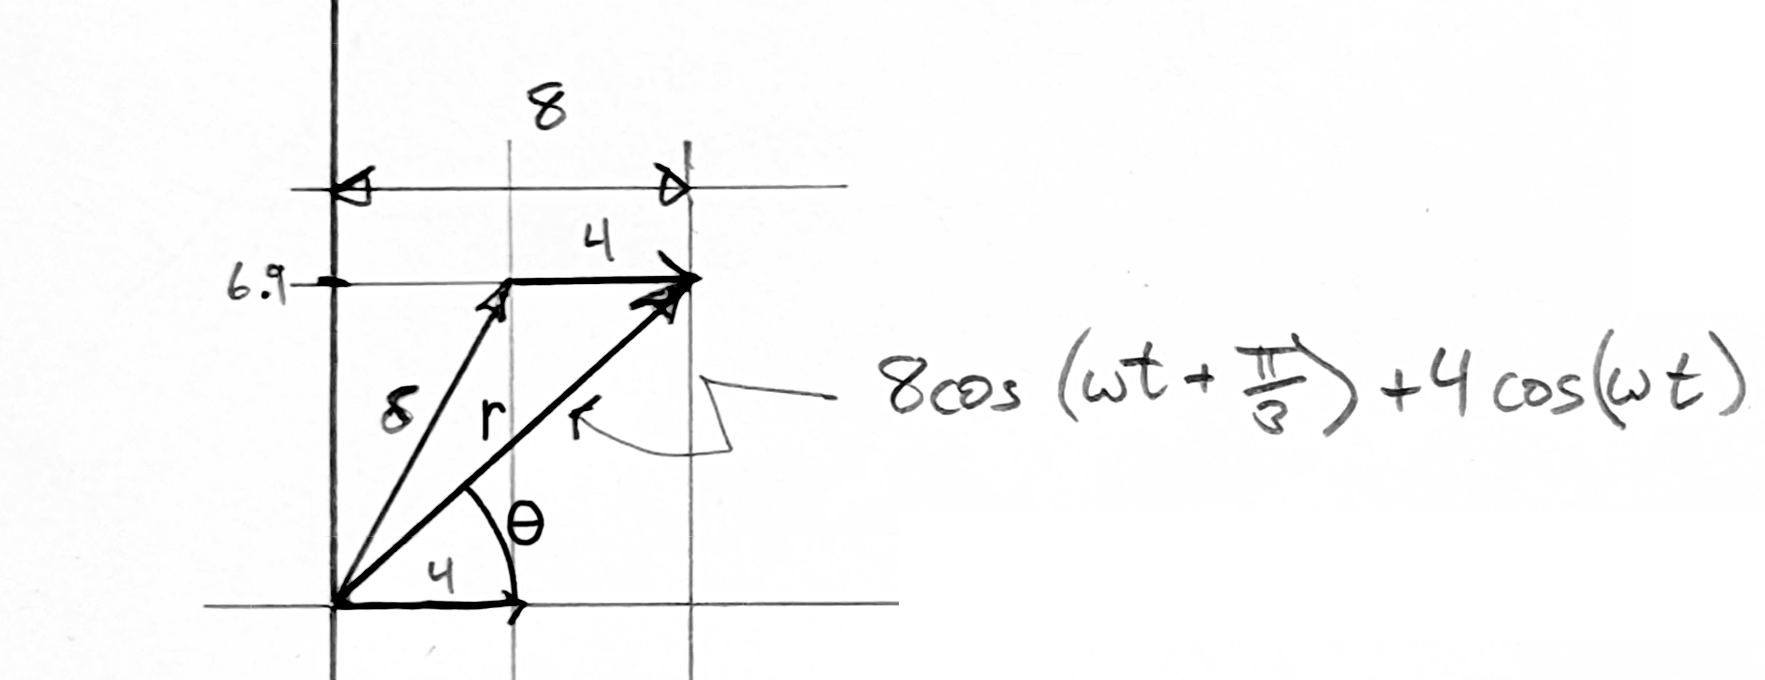
\includegraphics[width=.8\textwidth]{figsChapt02/NE94010.png}

\[
r = \sqrt{(8\sin(\pi/3))^2+8^2} = 10.56,\quad \theta = \mathrm{atan2}(6.9, 8) = 40.8^\circ
\]



\section{LODE Analysis of Electric Circuits  }


First we start with the
``Conventional Method'' (from the 1800's and early 1900's).   This will involve writing
a linear ordinary differential equation (``LODE'') for the circuit, and solving using
older techniques such as assuming the form of a solution and solving for constants.
Such solutions are often divided into two components which are added to get the solution:  the ``Forced Response''
and the ``Natural Response''.

The Forced Response is mathematically of the same form as the input to the circuit. For example,
if a DC voltage is supplied to the circuit via a switch thrown at $t=0$, the forced response
has the form of a   step function.

The Natural Response has the form that depends on the system properties.  For example,
a system which resonates in response to a transient input may have a transient response consisting
of a sinusoid which is multiplied by a damping function so that it disappears (declines in amplitude)
over time such as
\[
v_{NR}(t) =e^{-.1t} [ 10 \sin(45t+\pi/6) ]
\]
By about $t=100$, the $e^{-.1t}$ term is negligible and $v_{NR}(t)\approx 0$.


\paragraph{Steady State Case:}
Sometimes we care mostly about the transient ``Natural Response'', but other times (like this chapter) we care primarily
about the  ``Forced Response''.   A big application of sinusoidal steady state analysis is power
systems.  Although transients in power are also important, many loads are running far longer than
their transient time constants --- much more energy is consumed in the steady state when you turn
on a light bulb and run it for 12 hours.



\subsection{An Electrical AC Circuit}

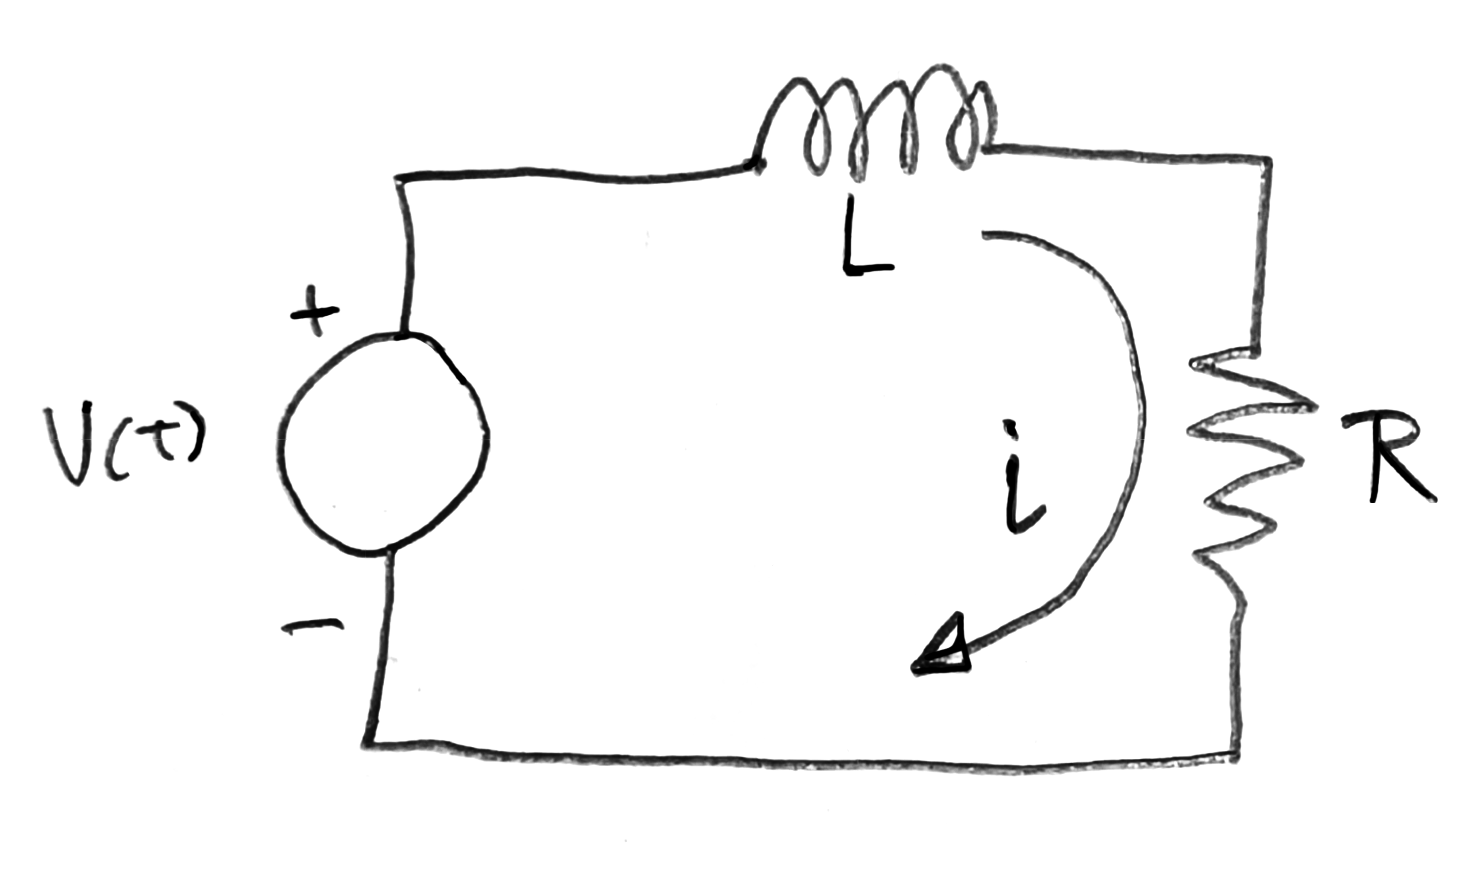
\includegraphics[width=0.5\textwidth]{figsChapt02/DI63347.png}


The traditional method for solving the response of a LODE system to sinusoidal input is roughly
introduced.

\noindent
First we take a high level look at the method:

\begin{enumerate}
\item Our Differential equation is:
\[
V(t) = L\frac{di}{dt} + iR
\]
(which is a L.O.D.E)

\item {\it assume} $\hat{i} = A\cos\omega t + B\sin\omega t$

\begin{quotation}
Q: Why is that a good assumption?

A: Because $\frac{d}{dt}\sin(x) = \cos(x)$, $\frac{d}{dt}\cos(x) = -\sin(x)$

Q: What about ``natural response''?

A: Were ignoring it!

Q: Why can we ignore natural response?

A: Because here we are studying only ``steady state response'' ... by definition this is
the same functional form as the forced response.
\end{quotation}

\item Plug   $\hat{i}$ into the LODE.

\item Evaluate derivative(s) in the LODE, collect $\sin$, $\cos$ terms

\item Solve for $A$, $B$ in terms of constants or variables in the LODE such as $R$, $L$, $V_M$, $\phi$

\item Massage the result into form $\underline{I}\cos(\omega t + \phi)$
if desired.
\end{enumerate}

\vspace{0.25in}

\noindent
Now the details:

\begin{enumerate}
\item Our LODE is:
\[
V_M\cos\omega t = L\frac{di}{dt} + iR
\]

\item We assume the solution is:
\[
\hat{i} = A\cos\omega t + B\sin\omega t
\]

\[\frac{d\hat{i} } {dt} = -A\omega\sin\omega t + B\omega\cos\omega t
\]

\item
\[
V_M\cos\omega t = -A\omega L\sin\omega t + B\omega L\cos\omega t + AR\cos\omega t + BR\sin\omega t
\]

\item
\[
V_M\cos\omega t = (BR - A\omega L)\sin\omega t + (AR + B\omega L)\cos\omega t
\]

Collecting the terms and equating like trig functions:
\[
BR - A\omega L = 0
\]

\[
AR + B\omega L - V_M = 0
\]

\item
\[
A = \frac{RV_M} {R^2 + \omega^2L^2}
\]

\[
B = \frac{\omega LV_M}{R^2 + \omega^2L^2}
\]

\[
i = \frac{V_M}{R^2 + \omega^2L^2}[R\cos\omega t + \omega L\sin\omega t]
\]

\item Convert to 2 cosine waves with trig identity; Vector addition

\[
R\cos\omega t + \omega L\sin\omega t = R\cos\omega t + \omega L\cos(\omega t - \pi/2)
\]

\noindent Result:

$\sqrt{R^2 + \omega^2L^2}\cos(\omega t + \tan^{-1}(\omega L/R))$

$\omega L\cos(\omega t - \pi/2)$

$i = \frac{V_M}{\sqrt{R^2 + \omega^2L^2}}\cos(\omega t - \tan^{-1}(\omega L/R))$
\end{enumerate}

\noindent
{\bf Pretty painful!}




\section{Complex Sinusoids and Phasors  }

Consider the a complex time function:  $e^{j\omega t}$
Using Euler's equation\footnote{BTW, Euler's equation is very easy to prove using the Taylor series
expansions of $e^x, \cos(x), \sin(x)$},

\[
e^{j\omega t} = \cos(\omega t) + j\sin(\omega t)
\]

More generally
\[
Ae^{j(\omega t + \phi)} = A\cos(\omega t + \phi) + jA\sin(\omega t + \phi)
\]

We call this a ``complex sinusoid''.
The real part and the imaginary part are
both sinusoids and they are $\pi/2$ out of phase because $\sin(x) = \cos(x+\pi/2)$.

Recall that the real part of a complex number is plotted on the $x$ axis
of the complex plane (often called the real axis) and the imaginary part
on the $y$ axis (often called the imaginary axis).   So the complex sinusoid
is also a vector in the complex plane
of magnitude $A$ rotating counter-clockwise around the origin ($0+j0$),
and if $V$ is a complex sinusoid, $Ae^{j(\omega t+\phi)}$,
then $\text{Re}\{V\} = A\cos(\omega t + \phi)$
which is a regular sinusoid.

We will find complex sinusoids quite useful to simplify the process of solving
for AC sinusoidal steady state responses of circuits.


\subsection*{Better Method - Phasors (Steinmetz - not Star Trek!)}

Developed by Charles Steinmetz in 1893, we
define a {\it phasor}, $\vec{P}$ as
\[
    \vec{P} = P_M e^{j\phi}
\]

``Phasor'' is a contraction of ``PHASE vecTOR,''
but it also encodes amplitude, $P_M$.

Let's go back to the complex sinusoid
\[
Ae^{j(\omega t + \phi)} = A\cos(\omega t + \phi) + jA\sin(\omega t + \phi)
\]

We can factor the LHS above as
\[
e^{j(\omega t)}Ae^{j\phi} = e^{j(\omega t)}\vec{P}
\]
where $\vec{P}=P_Me^{j\phi}$ is the phasor which breaks down a complex
sinusoid into the product of a phasor and a
complex sinusoid of unit mag at zero phase.

The physical variable such as sinusoidal voltage or current is represented by
the {\bf real} part of the complex sinusoid,
 $\text{Re}\{V_M e^{j\phi} \cdot e^{j\omega t}\} = \text{Re}\{V_M e^{j(\omega t+\phi)}\}$
= $V_M\cos(\omega t + \phi)$

To clarify, we note that the {\bf phasor} is just a complex number:
\[
\vec{P} = a + jb
\]
and the {\bf complex sinusoid} is (assuming it is a voltage):
\[
\vec{V(t)} = \vec{V}e^{j\omega t} = V_Me^{j\phi}e^{j\omega t} = V_M [\cos(\omega t + \phi)+j\sin(\omega t + \phi)]
\]
The phasor encodes the magnitude and phase of the sinusoid but not its frequency. Also, the
complex sinusoid is a time function and the phasor is a complex constant.

\begin{ExampleSmall}
What Phasor corresponds to the sinusoidal physical voltage:
$V(t) = V_M\cos(\omega t + \phi)$?

\vspace{0.25in}
\paragraph{Solution:}
The corresponding complex sinusoid version is
\[
V(t) =\text{Re}\{V_M[\cos(\omega t+\phi) + j\sin(\omega t+\phi)]\} = V_M\cos(\omega t+\phi)
\]
Starting with the complex sinusoid, we use the fact that a phasor encodes the magnitude and phase
but not $\omega t$.
Writing the phasor form of our complex sinusoid:
\[
    V_M[\cos(\omega t+\phi) + j\sin(\omega t+\phi)] = V_M e^{j(\omega t+\phi)}
     = V_M e^{j\phi}e^{j\omega t}
     = \vec{V}e^{j\omega t}
\]
thus the phasor corresponding to $V(t)$ is
\[
\vec{V}=V_Me^{j\phi}
\]

\end{ExampleSmall}
\vfill

\begin{ExampleSmall}
What phasor corresponds to:
\[
I(t) = \cos(\omega t+\pi/4) + 2\sin(\omega t)
\]


\paragraph{Solution:} The two terms can be expressed as complex sinusoids from
which we derive phasors:

\noindent{1) First, we use our knowledge of trig functions to convert the original
function to:}

\[
I(t) = \cos(\omega t+\pi/4) + 2\cos(\omega t-\pi)
\]

$\cos(\theta)$ is the function which gives the real part of complex sinusoids.

\noindent{2)}
\[
\cos(\omega t+\pi/4)= \text{Re}\{e^{j\omega t}\vec{P_1}\}
\]
where $P_1 = 1e^{j\pi/4} = 0.707 + j0.707$.


\noindent{3)}
\[
2\cos(\omega t-\pi) = \text{Re}\{e^{j\omega t}\vec{P_2}\}
\]
where $P_2 = 2e^{j(-\pi)} = -2 + j0$.

We can also put the original complex sinusoid together as
\[
    I(t) = \text{Re}\{e^{j\omega t}\vec{P_1}+e^{j\omega t}\vec{P_2}\}
    \]

Now, comes the key benefit of phasors: we can factor out the first term of each
sinusoid:

\[
I(t) = \text{Re}\{e^{j\omega t}\left (
        \vec{P_1}+\vec{P_2}
        \right ) \}
\]
\[
\vec{P_1}+\vec{P_2} = -1.293 + j0.707
\]
so the phasor corresponding to $\vec{I}$ is $ -1.293 + j0.707$,
\[
|\vec{I}| = \sqrt{-1.293^2+.707^2} = 4.716
\]
\[
\angle{\vec{I}} = \mathrm{atan2}(.707, -1.293) = 151.3^\circ  =2.641
\]
So our phasor is
\[
\vec{I}(t) = 4.716e^{j2.641}
\]

We have reduced the problem of adding two sinusoids of different magnitudes and
phases (but not different frequencies) to adding two complex numbers.
\end{ExampleSmall}



\begin{ExampleSmall}\label{firstPhasorCktKVL}

Now we go back to the same RL circuit:

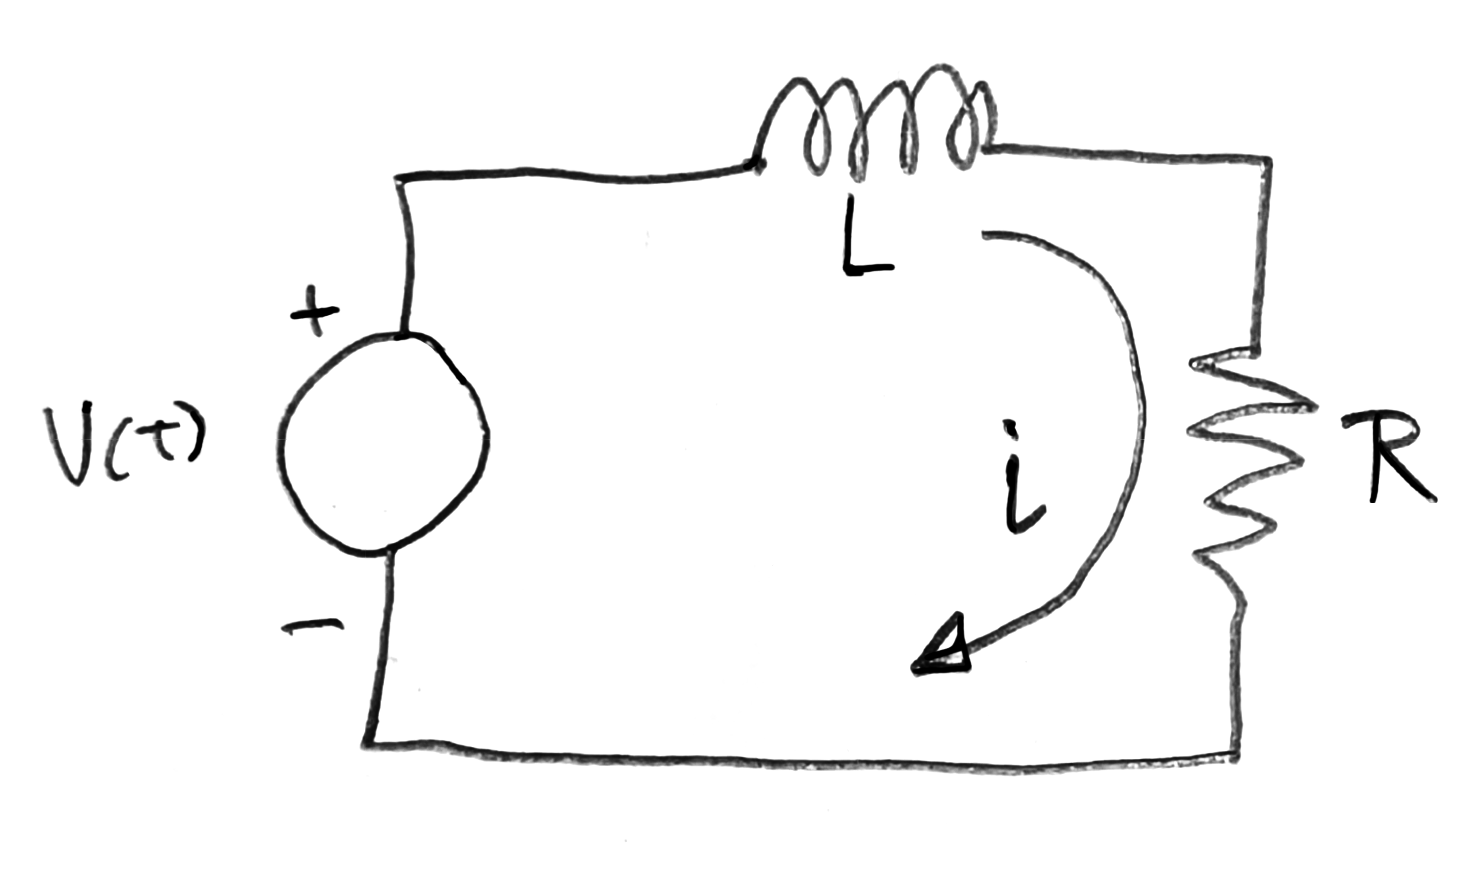
\includegraphics[width=0.5\textwidth]{figsChapt02/DI63347.png}

\begin{enumerate}
\item Summing the  voltages around the loop:

\[
V_M\cos(\omega t) - L\frac{di}{dt} - iR = 0
\]

\[
V_M\cos(\omega t) = L\frac{di}{dt} + iR
\]

\item Consider input voltage to be the real part of a complex phasor:

\[
V_M\cos(\omega t) = \mathrm{Re}\{ \vec{V}e^{j\omega t} \}
\]
And we define
\[
i(t) = \mathrm{Re}\{ \vec{I}e^{j\omega t}  \}
\]
as the current phasor which is
unknown.

% \noindent $\{i \cdot \vec{V}, \vec{I}, V_0\}$

\item We plug the unknown current and voltage phasors into (1)

\[
\vec{V}e^{j\omega t} = j\omega L\vec{I}e^{j\omega t} + R\vec{I}e^{j\omega t}
\]
(the leading $j\omega$ term on the RHS comes from differentiating as in the original LODE).


\item We can skip steps 4-6 of the previous method by
simply factoring out and cancelling $e^{j\omega t}$ from all the terms!
\[
\vec{V} = j\omega L\vec{I} + R\vec{I}
\]
(the big speedup comes when we learn to write this from
directly looking at the circuit)

We often assume zero phase angle for input sinusoids so in this (common) case we have
\[
\vec{V} =V_Me^{j0} = V_M
\]
\end{enumerate}
\end{ExampleSmall}

\begin{ExampleCont}

Solving the phasor equation we easily get:
\[
\vec{I} = \frac{\vec{V}}{  j\omega L + R}
\]

Let
\[
\phi = \tan^{-1}\left(\frac{\omega L}{R}\right)
\]
so
\[
\vec{I} = \frac{V_M}{\sqrt{R^2+\omega^2L^2}}e^{-j\phi}
\]

\[
= \frac{\vec{V}}{\sqrt{R^2+\omega^2L^2}} = \frac{V_M}{\sqrt{R^2+\omega^2L^2}}\cos(\omega t - \phi)
\]
Usually, all we really need to know is the magnitude and phase angle of our answer which we read
off directly from the phasor $\vec{I}$.
\end{ExampleCont}

Now we will directly apply the phasor method to a slightly different problem on
the same circuit:




\begin{ExampleSmall}


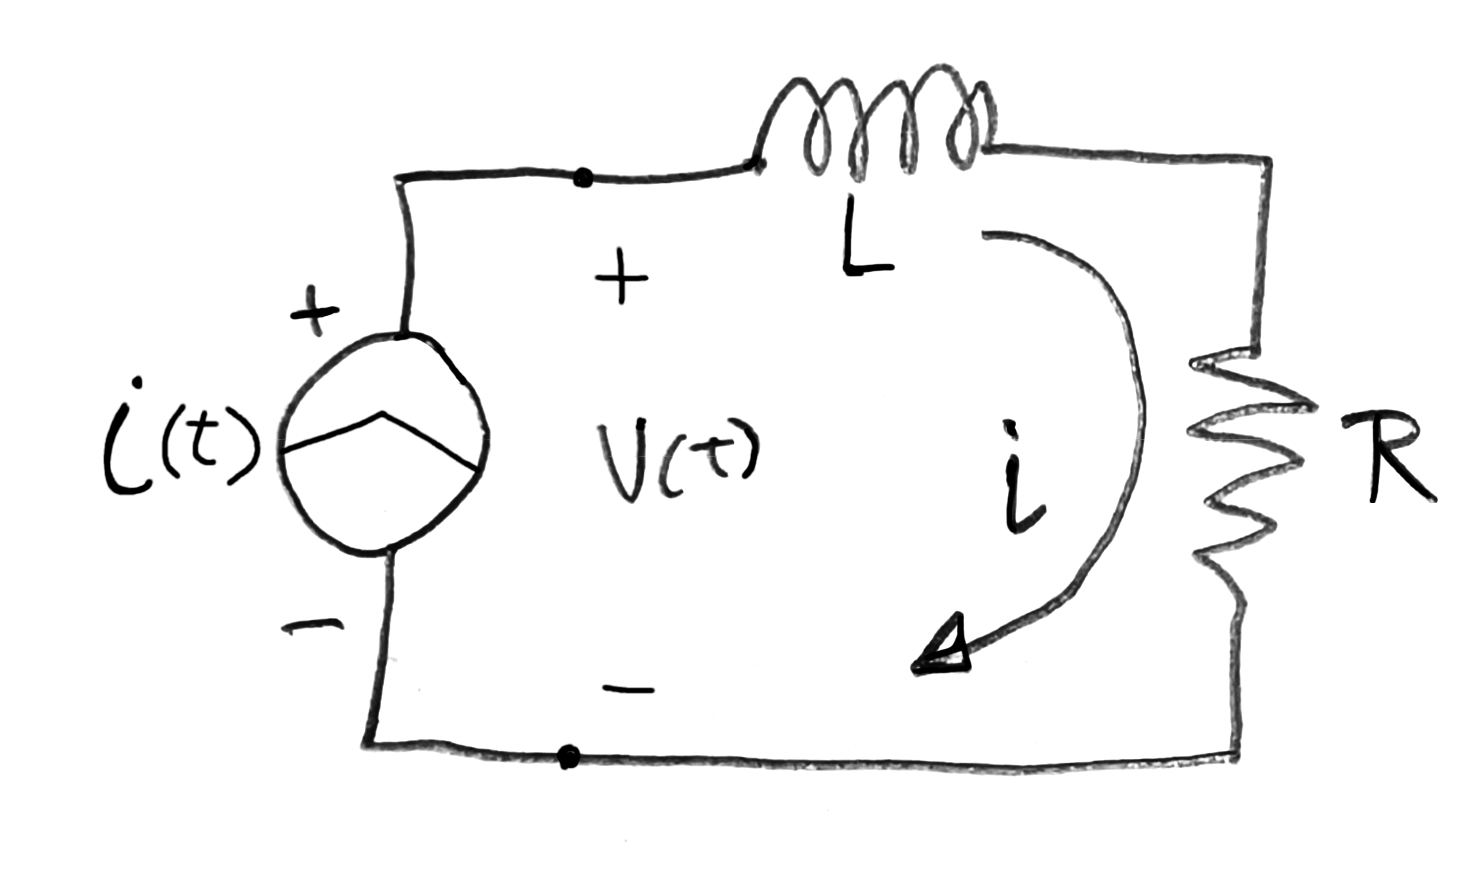
\includegraphics[width=0.5\textwidth]{figsChapt02/ND14529.png}

We drive the RL circuit this time with a current source having
\[
\vec{I} = I_me^{j0}
\]
Find the voltage $v(t)$ by the Phasor method.

\paragraph{Solution:}

Our new streamlined procedure for the steady state sinusoidal analysis is therefore
to compute each voltage drop by the product of the current phasor and the impedance,
and then write a KVL equation:
\begin{enumerate}
\item KVL Equation:

$+V_M\cos(\omega t) = L\frac{di}{dt} + \frac{1}{C}\int i\,dt + iR$

\item Convert voltage and currents to Phasor

$V_M\cos(\omega t) =$

$= \vec{V}e^{j\omega t} = \vec{I}e^{j\omega t}$

\item Plug in
\[
\vec{V}e^{j\omega t} = j\omega L\vec{I}e^{j\omega t} + \frac{1}{j\omega C}\vec{I}e^{j\omega t} + \vec{I}Re^{j\omega t}
\]


\end{enumerate}

\end{ExampleSmall}


\section{Phasor equations for energy storage components}


\subsection{Capacitor}



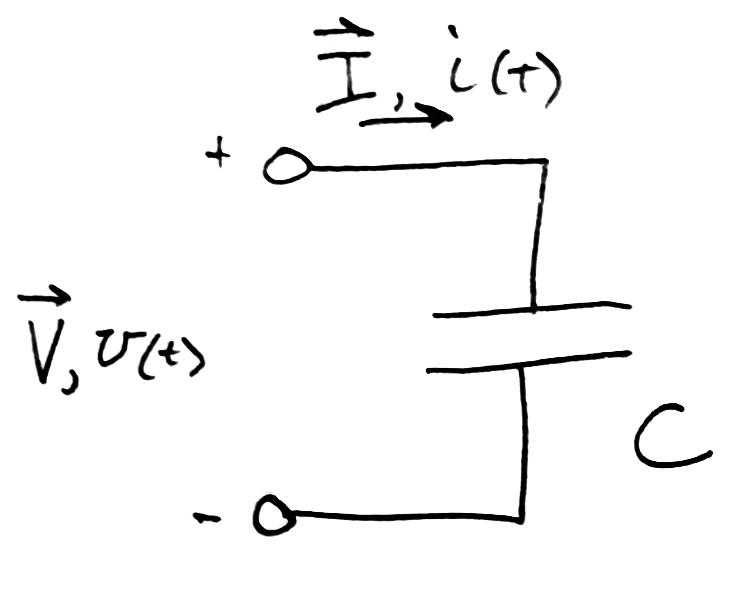
\includegraphics[width=0.35\textwidth]{figsChapt02/MI65790.png}

We know the differential equation relating voltage and current on a capacitor is
\[
v(t) = \frac {1}  {C}\int i(t) dt
\]
let's substitute a voltage complex sinusoid for the LHS, and plug in a complex sinusoid $\vec{I}e^{j\omega t}$
on the RHS:
\[
\mathrm{Re}\left \{\vec{V}e^{j\omega t} \right\} = \mathrm{Re}\left \{\frac {1}  {C}  \int \vec{I}e^{j\omega t} dt \right\}
\]

and
\[
\vec{V}e^{j\omega t} = \frac {1}  {C}  \int \vec{I}e^{j\omega t} dt
\]
integration gives
\[
\vec{V}e^{j\omega t} =  \vec{I}\frac {1}  {j\omega C}   e^{j\omega t}
\]
Finally, we cancel out the $e^{j\omega t}$ to get a phasor-only equation
\[
\vec{V} = \vec{I} \frac {1}  {j\omega C}
\]
this is a direct analog of Ohms law, $V=IR$ except
\begin{enumerate}
  \item  It uses a complex number ($ \frac {1}  {j\omega C}$) instead of the real number value of resistance, $R$,\vspace{0.2in}
  \item  It works for capacitors!   Up until now we had to solve differential equations.\vspace{0.2in}
  \item (remember, phasor analysis {\it assumes} sinusoidal steady state operation. Ohms law works all the time.)\vspace{0.2in}
\end{enumerate}
we will call the quantity $\vec{Z_C} =  \frac {1}  {j\omega C}$ the ``phasor impedance'' of the capacitor and we note:

\begin{enumerate}
  \item $\angle{Z_C} = -\pi/2$\\
  This means the current $\vec{I}$ {\bf leads} the voltage $\vec{V}$ by $\pi/2$ radians or $90^\circ$.\vspace{0.2in}
  \item $|Z_C| = \frac {1}  {\omega C}$\\[2mm]
  The higher the steady state frequency, $\omega$, or capacitance, $C$, the lower the magnitude of the impedance (and if voltage is fixed,
  the higher the current through the capacitor.)\vspace{0.2in}
\end{enumerate}

We can illustrate the two complex sinusoids, given by the equations
\[
\vec{V}e^{j\omega t}\;\; \vec{I}e^{j\omega t}
\]
as follows:

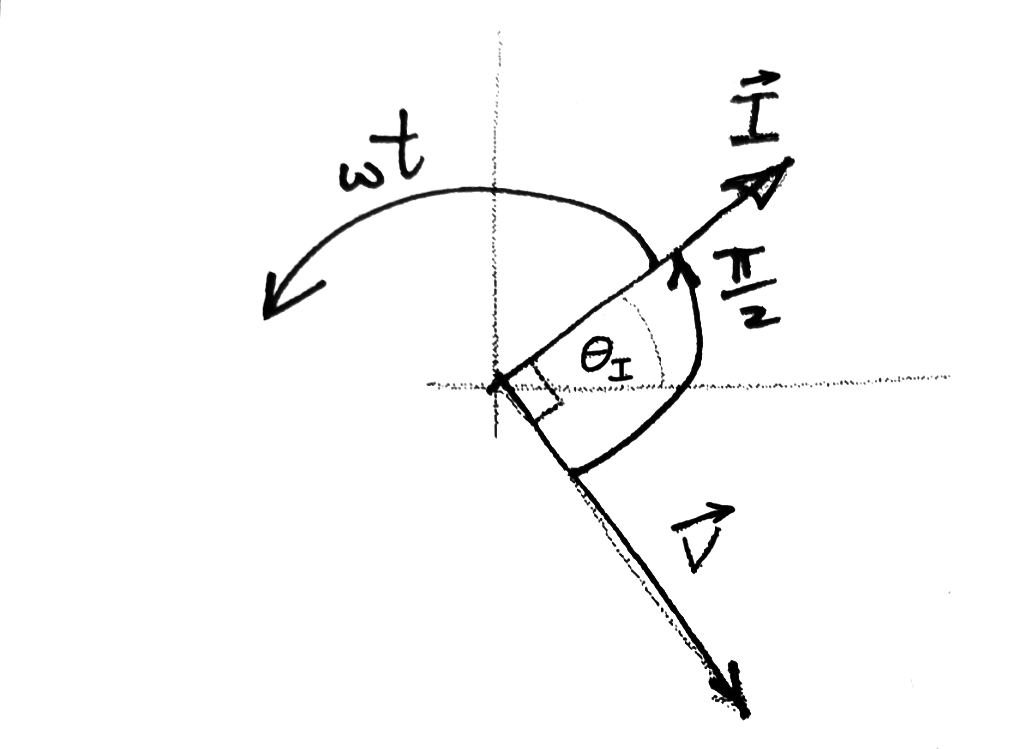
\includegraphics[width=0.35\textwidth]{figsChapt02/GM66229.png}



\subsection{Inductor}
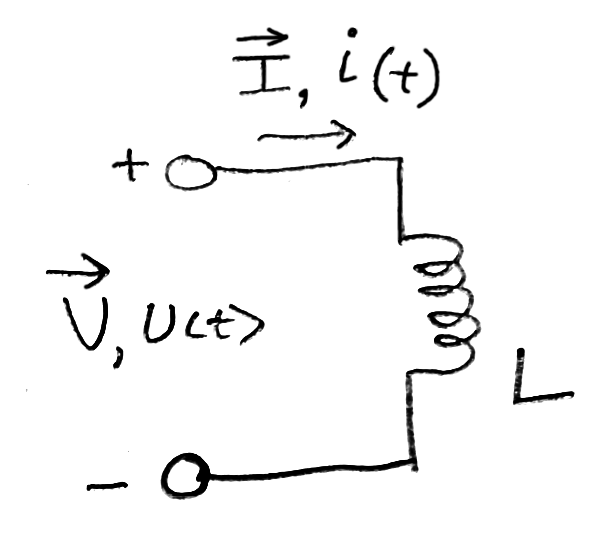
\includegraphics[width=0.35\textwidth]{figsChapt02/MP46579.png}

The analysis for the inductor is almost identical to the capacitor derivation directly above, except the consitutive equation
for the inductor is
\[
v(t) = L\frac {d}  {dt} \; i(t)
\]
so the resulting phasor impedance  equation is
\[
\vec{V} = j\omega L \vec{I}
\]
\[
Z_L = j\omega L,;\quad
\]

\begin{enumerate}
  \item $\angle{Z_L} = +\pi/2 = +90^\circ$\\
  This means the inductor current $\vec{I}$ {\bf lags} the voltage $\vec{V}$ by $\pi/2$ radians or $90^\circ$.
  \item $|Z_L| = \omega L$\\
  The higher the steady state frequency, $\omega$, or the inductance, $I$, the higher the magnitude of the impedance (and if voltage is fixed,
  the smaller the current through the inductor.)
\end{enumerate}

The vector diagram corresponding to the capacitor diagram above is the same except that the voltage would {\bf lead} the current.


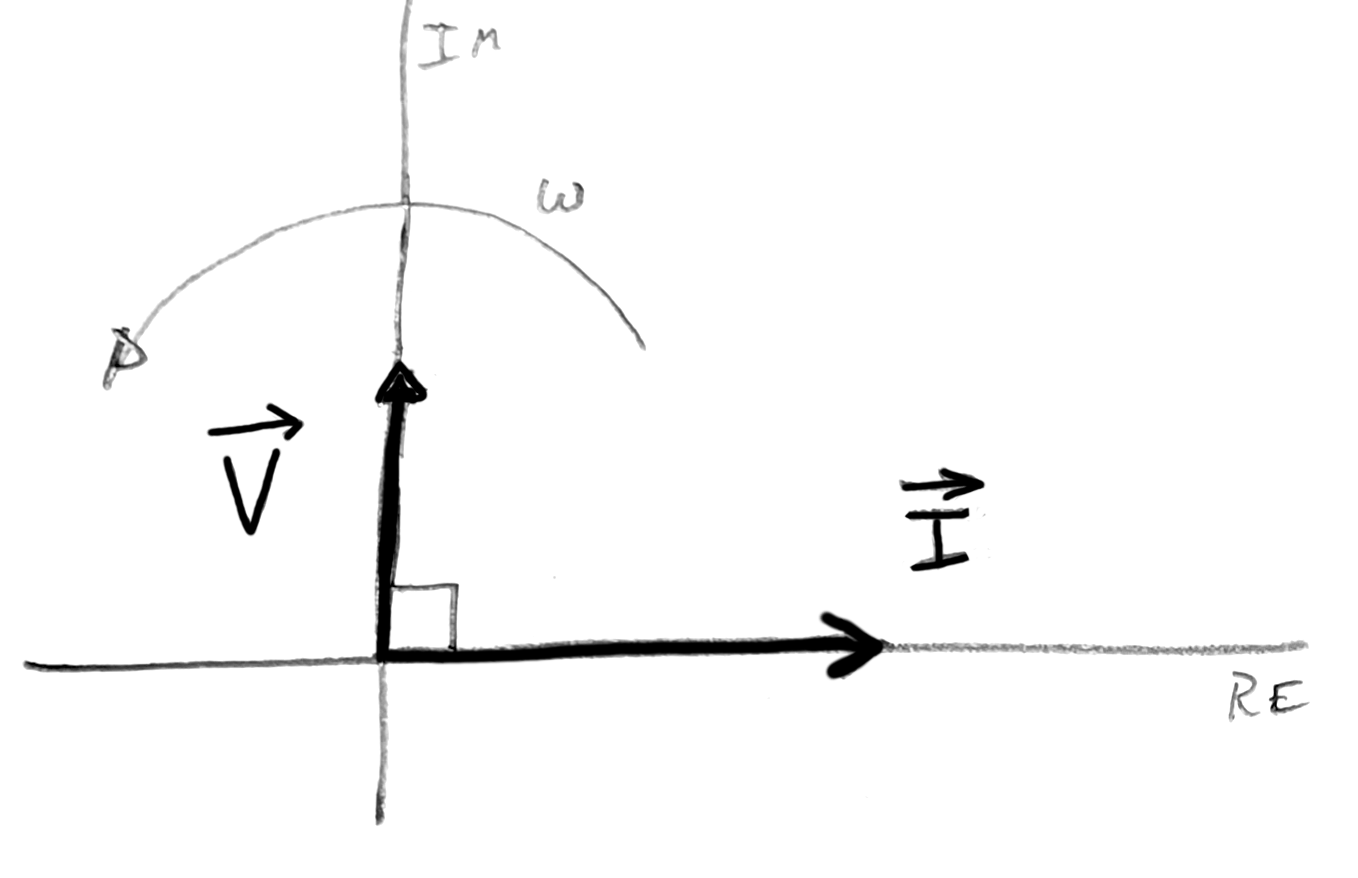
\includegraphics[width=0.35\textwidth]{figsChapt02/EC64016.png}
The resulting sinuoids can be sketched

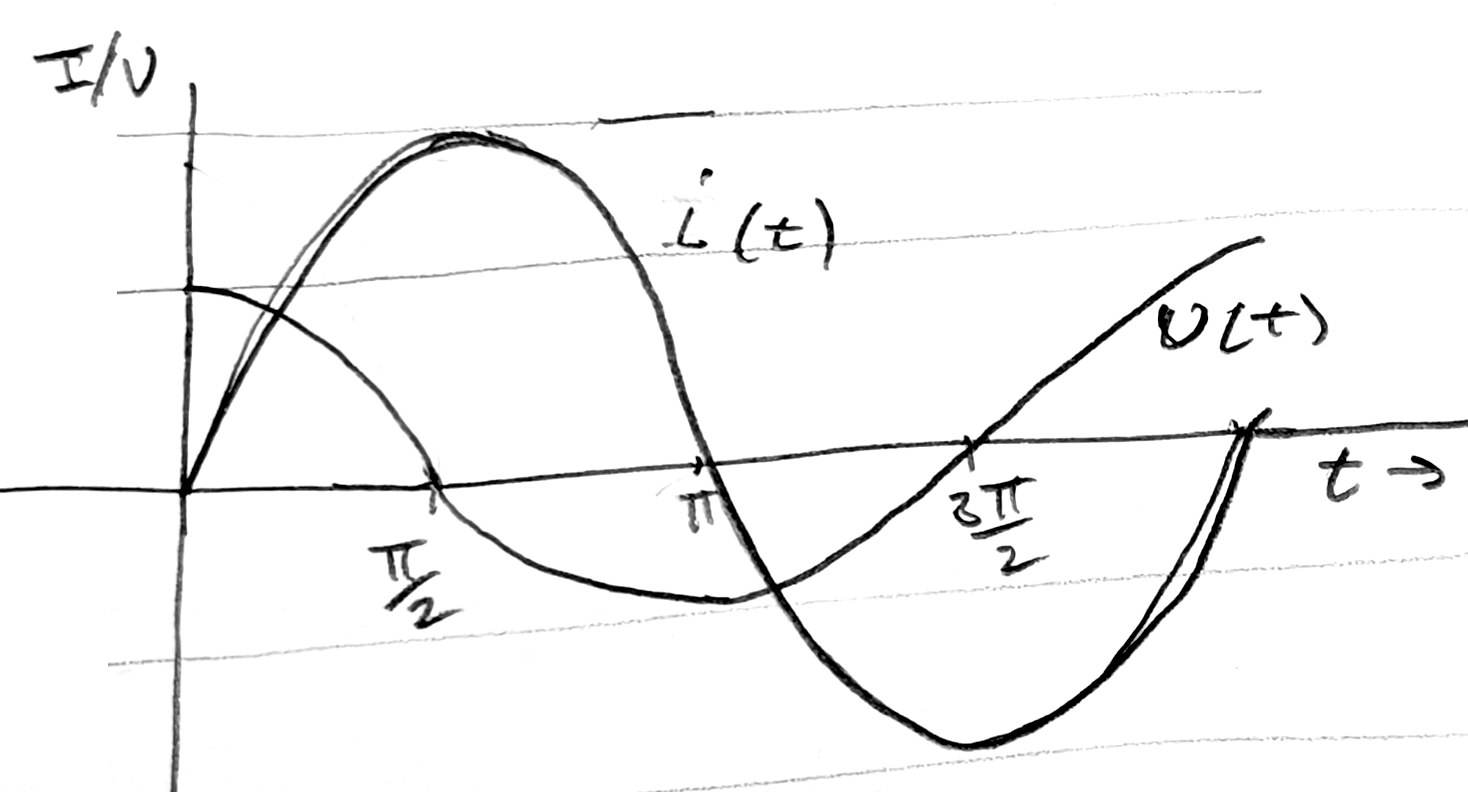
\includegraphics[width=0.35\textwidth]{figsChapt02/PP03048.png}


\section{Impedance}

We have now found complex quantities analogous to resistance for the energy storage elements, specifically

\begin{align}
\mathrm{Inductor:}  & \vec{V} = j\omega L \vec{I}\\
\mathrm{Capacitor:}  & \vec{V} = \frac{1}{j\omega C} \vec{I}\\
\end{align}
We also then have:
\[
\vec{V} = Z\vec{I}
\]
were
\[
Z = \frac {\vec{V}}  {\vec{I}}
\]
$Z$ is called ``complex impedance'' or simply ``impedance''.

We also define:
\[
\mathrm{Re}\left\{ Z\right\} = \mathrm{Resistance, ~R}
\]
\[
\mathrm{Im}\left\{ Z\right\} = \mathrm{Reactance, ~X}
\]
(note that 'R' was already taken when they had to abbreviate ``Reactance''!).

Reactance has two ``flavors'' based on it's sign.   Because
\[
X_C = \frac {-1}  {\omega C}
\]
and $\omega, C$ are always positive, we call any $X<0$ ``Capacitive Reactance''. Similarly
we call $X>0$ ``Inductive reactance'' since
\[
X_L = \omega L
\]
which is also always positive.


\subsection{Recap:}
Complex impedance, $Z$, is defined in terms of the phasors, $\vec{I}, \vec{V}$ as:
\[
Z = \frac {\vec{V}}  {\vec{I}}
\]
For inductance and capacitance, we have
\[
Z_L = j\omega L,\;\; Z_C = \frac {1}  {j\omega C}
\]
We introduced another new term, ``Reactance'', $X$, which is the imaginary part of $Z$.
\[
Z = R + jX
\]

For inductors and
capacitors, the reactances are:
\[
X_L = \omega L\;(\angle{Z_L} = \pi/2),\;\; X_C = -\frac {1}  {\omega C}\; (\angle{Z_C} = -\pi/2)
\]

\subsection{Related quantities: Admittance, Conductance, Susceptance}

\paragraph{Admittance}
Just as Conductance is $1/R$, we define Admittance, $Y$, as a complex number
which is the inverse of Impedance
\[
Y = \frac {1}  {Z} = \frac{1}{R+jX} = G+jB
\]
Note that you can derive that
\[
Y = \frac {R-jX}  {|Z|^2}
\]
(try it using properties of complex numbers).


\paragraph{Conductance and Susceptance}

The new letters in the complex value of Admittance are
\begin{align}
\mathrm{G} &= \mathrm{Re}\left \{ Y \right \} = \mathrm{Conductance}\\
\mathrm{B} &= \mathrm{Im}\left \{ Y \right \} = \mathrm{Susceptance}
\end{align}
(Note that unless $B=0$, $G \neq 1/R$!)


\subsection{}






\section{Using Phasors in Circuit Analysis }




\subsection{Series and Parallel Impedances}

Nicely, these work exactly the same as resistances:

\paragraph{Series Combinations}
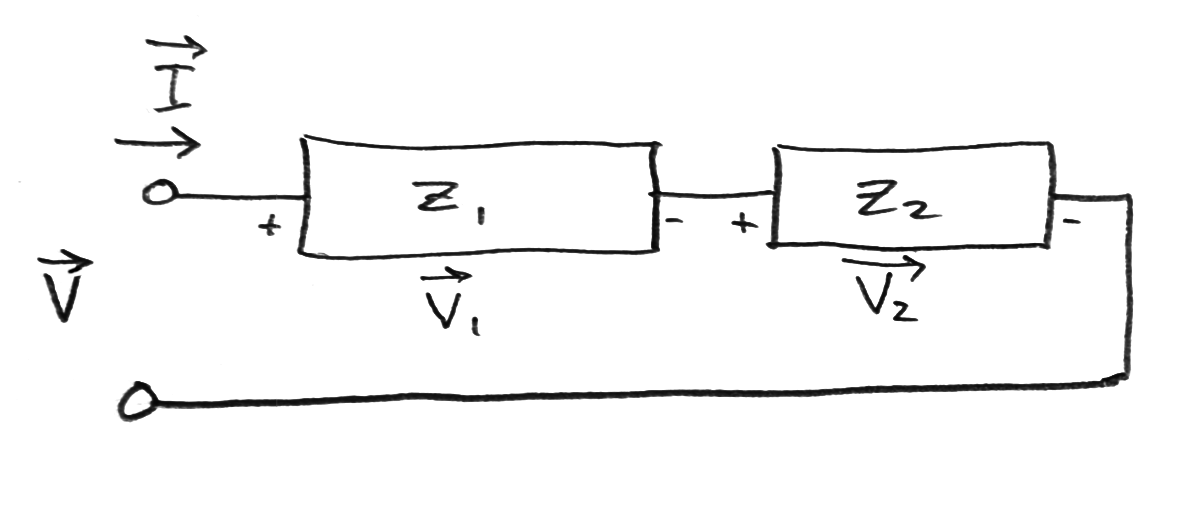
\includegraphics[width=0.3\textwidth]{figsChapt02/FT71566.png}

\[
\vec{V} = \vec{V}_1  + \vec{V}_2
\]
\[
\vec{V} = Z_1\vec{I}  + Z_2\vec{I} = \vec{I}(Z_1+Z_2)
\]
So series impedances combine by addition.

\paragraph{Parallel Combinations}
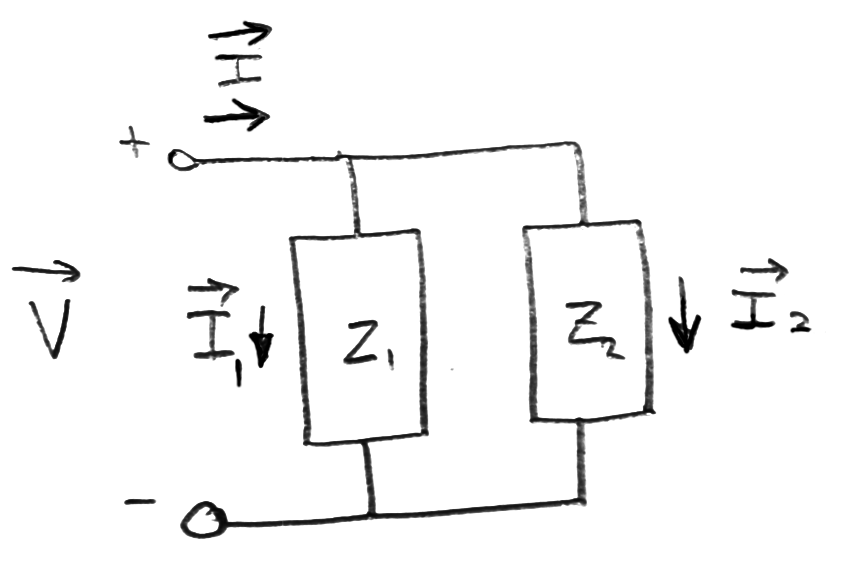
\includegraphics[width=0.3\textwidth]{figsChapt02/IM00849.png}

\[
\vec{V} = \vec{I}_1 Z_1 =  \vec{I}_2 Z_2
\]
\[
\vec{I} = \vec{I}_1 +  \vec{I}_2
\]
\[
Z_{tot} = \frac {\vec{V}}  {\vec{I}}
= \frac {\vec{V}}  {\frac {\vec{V}}  {Z_1} + \frac {\vec{V}}  {Z_2} }
\]
\[
Z_{tot} = \frac {1}  {\frac {1}  {Z_1}  + \frac {1}  {Z_2}  }
\]

Parallel impedances combine like parallel resistances:
\[
Z_{par} = \frac {1}  {\sum\limits_{i} \frac {1}  {Z_i} }
\]





\section{Circuit Examples}


\subsection{RL Circuit}\label{seriesRLckt}

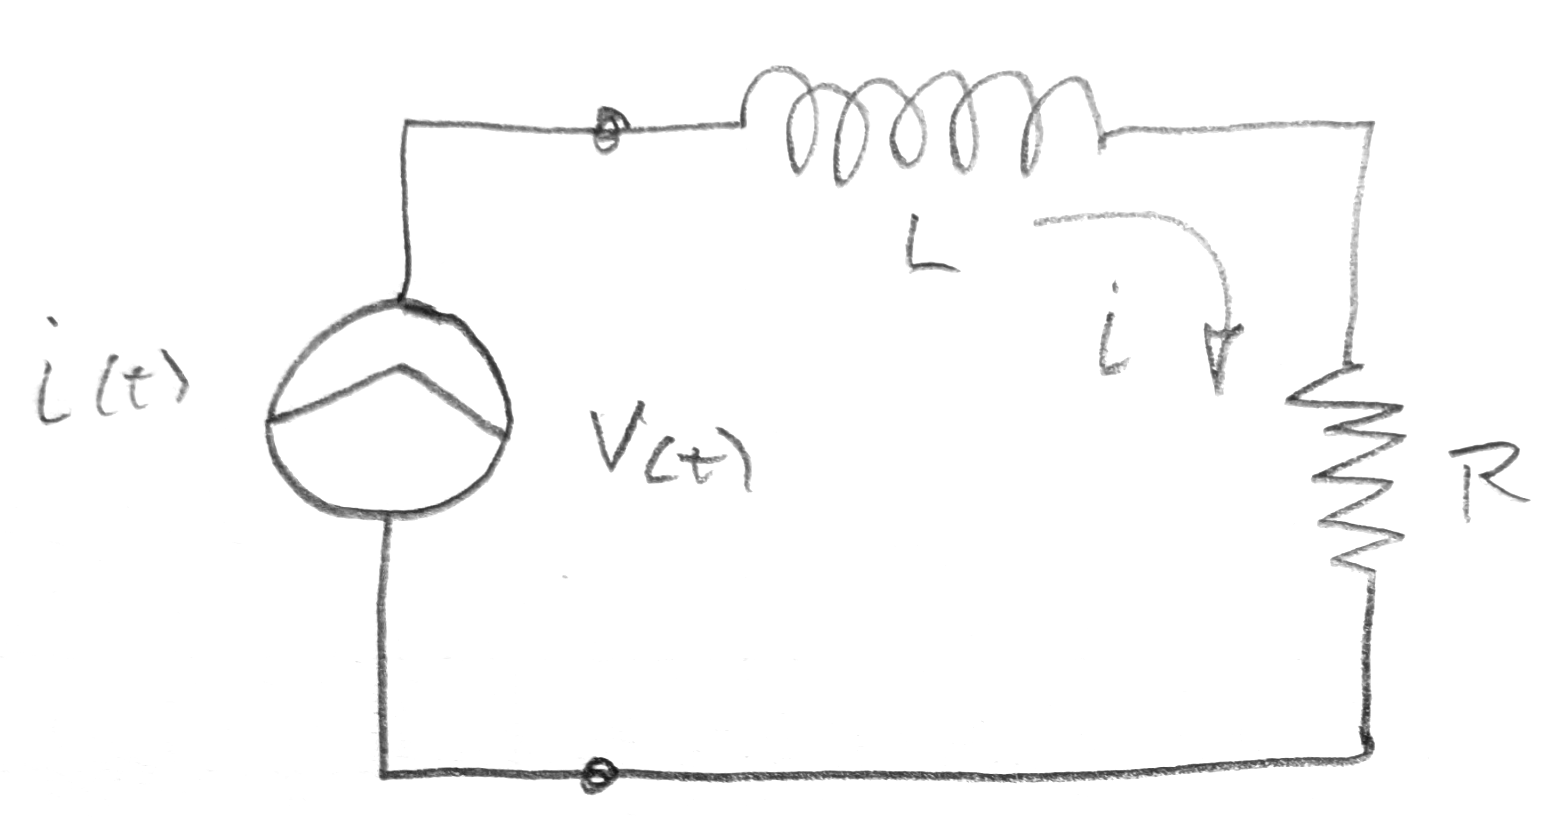
\includegraphics[width=0.5\textwidth]{figsChapt02/RI98726.png}

\paragraph{Problem:} Find $\vec{V}$ and $v(t)$ by the phasor method.
\paragraph{Solution:}
Deriving the current phasor:
\[
i(t) = I_M\cos(\omega t),\;\; \vec{X} = I_Me^{j0} = I_M
\]

1)
Evaluate phasor voltage drops and combine them via KVL
\[
\vec{V} = j\omega L \vec{X} + \vec{X} R
\]

2) Solve for $\vec{V}$:
\[
\vec{V} = \vec{X} (R+j\omega L)
\]
\[
\vec{V} = I_MR + jI_M \omega L
\]
\[
|\vec{V}| = \sqrt{I_M^2 R^2 + I_M^2(\omega L)^2} \equiv V_M = I_M\sqrt{R^2+(\omega L)^2}
\]
\[
\angle{\vec{V}} = \tan^{-1}(\frac {\omega L}  {R} ) \equiv \theta
\]
\[
\vec{V} = V_Me^{j\theta}
\]

note  $\vec{V} = \vec{X}(R+j\omega L) $ is just like Ohms Law, $V=IR$ if that $R$ were complex.

Since the complex reactances have their own directions (in the complex plane), we can diagram the summation


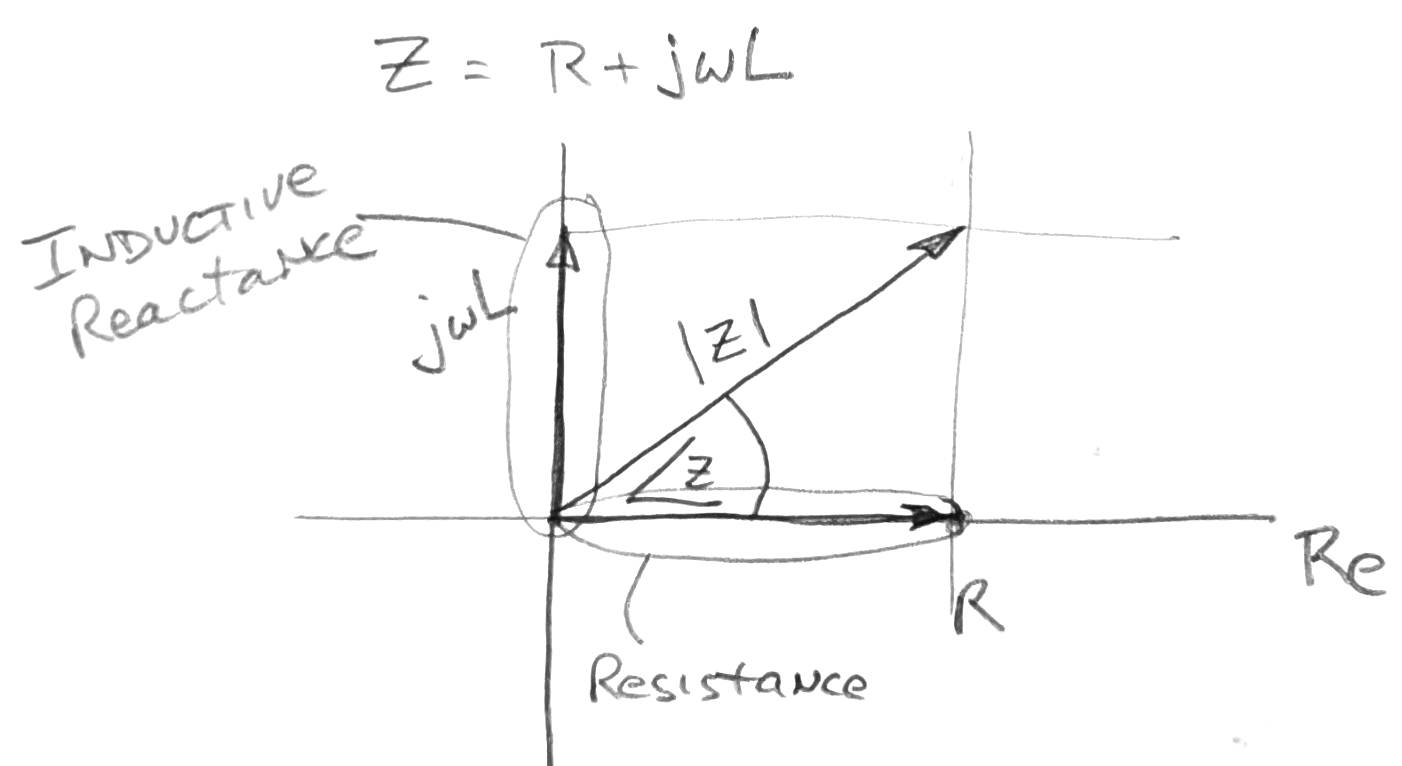
\includegraphics[width=0.5\textwidth]{figsChapt02/UI87197.png}

The imaginary part of the impedance is $j\omega L$, and the real part is $R$.
If we also had a capcitor in the circuit, it would have a negative (aka ``capacitive") reactance,
and the diagram would look like

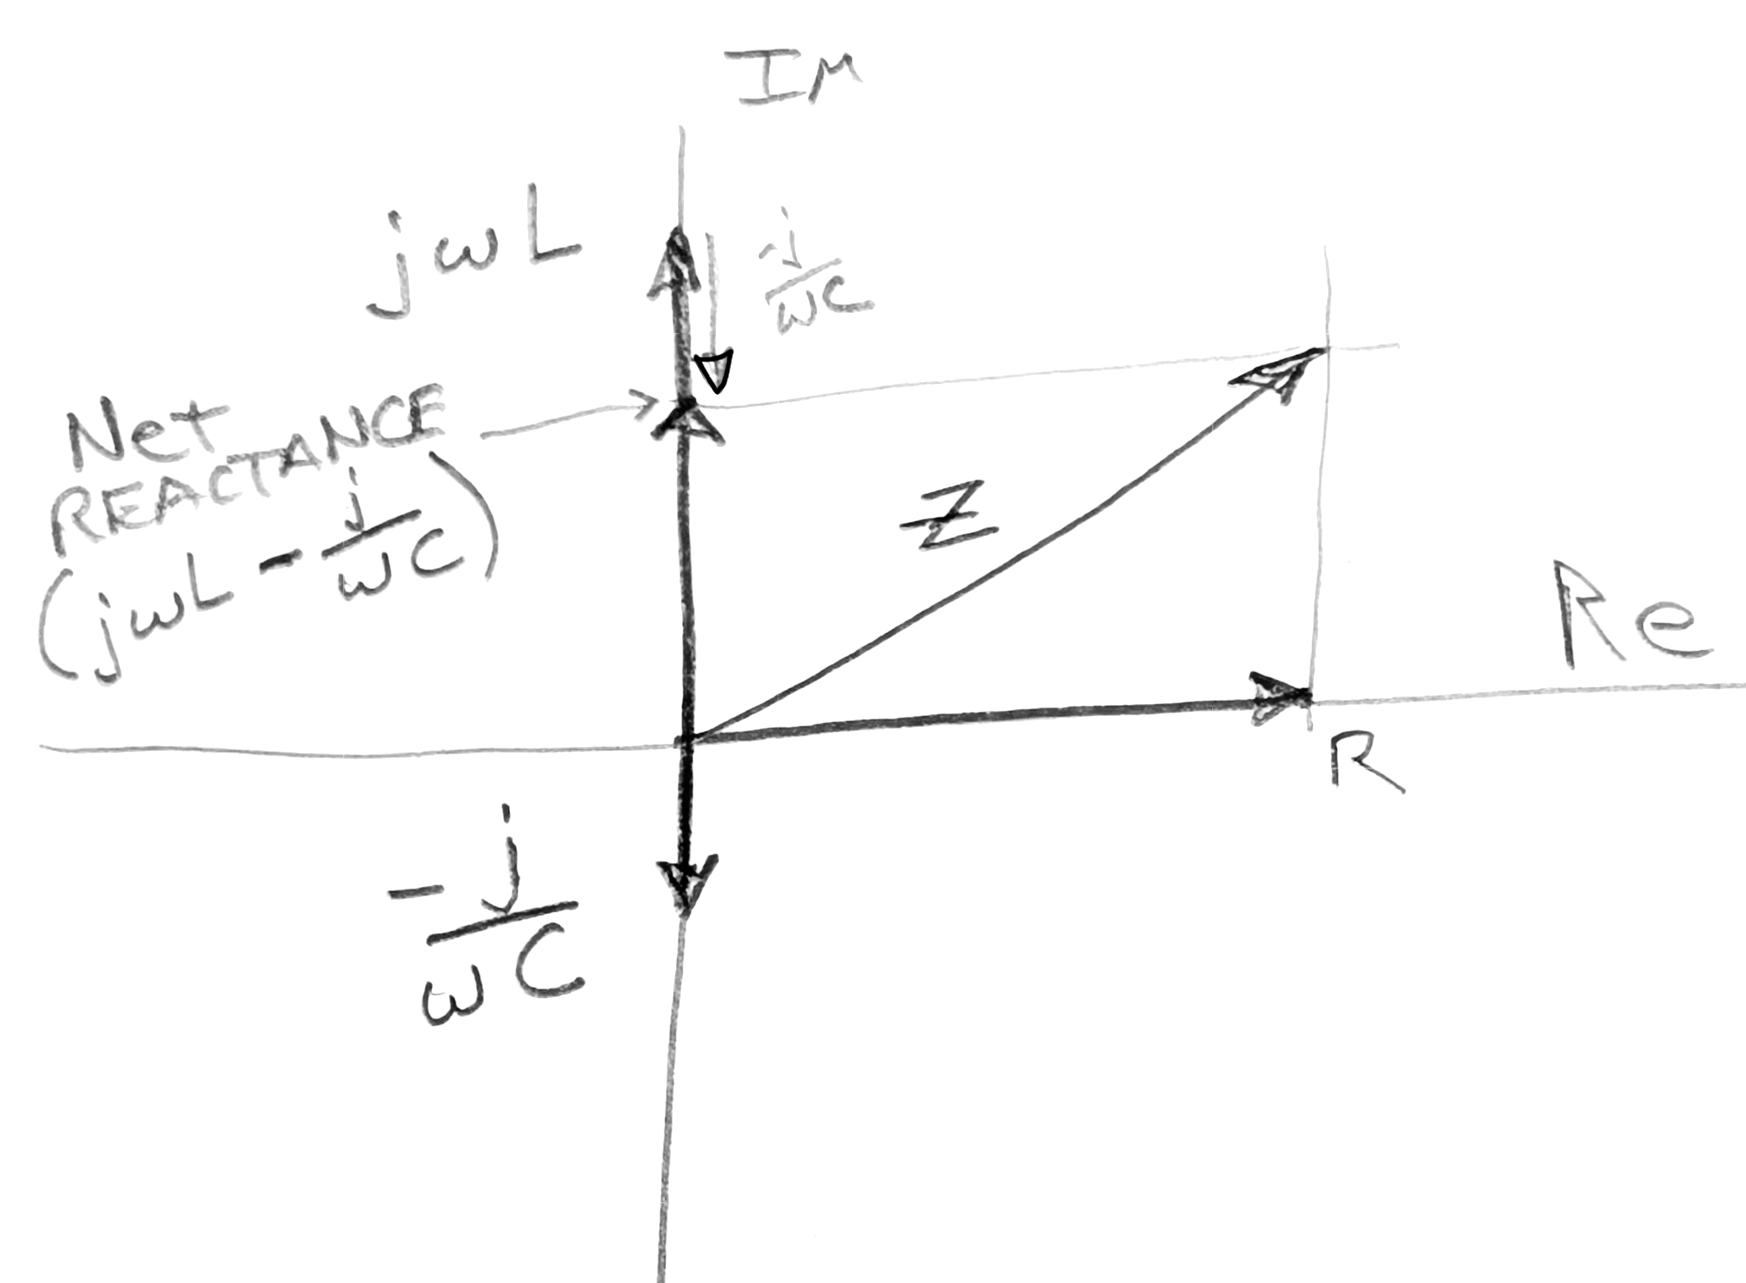
\includegraphics[width=0.5\textwidth]{figsChapt02/HF41781.png}

\subsection{More complex circuit}

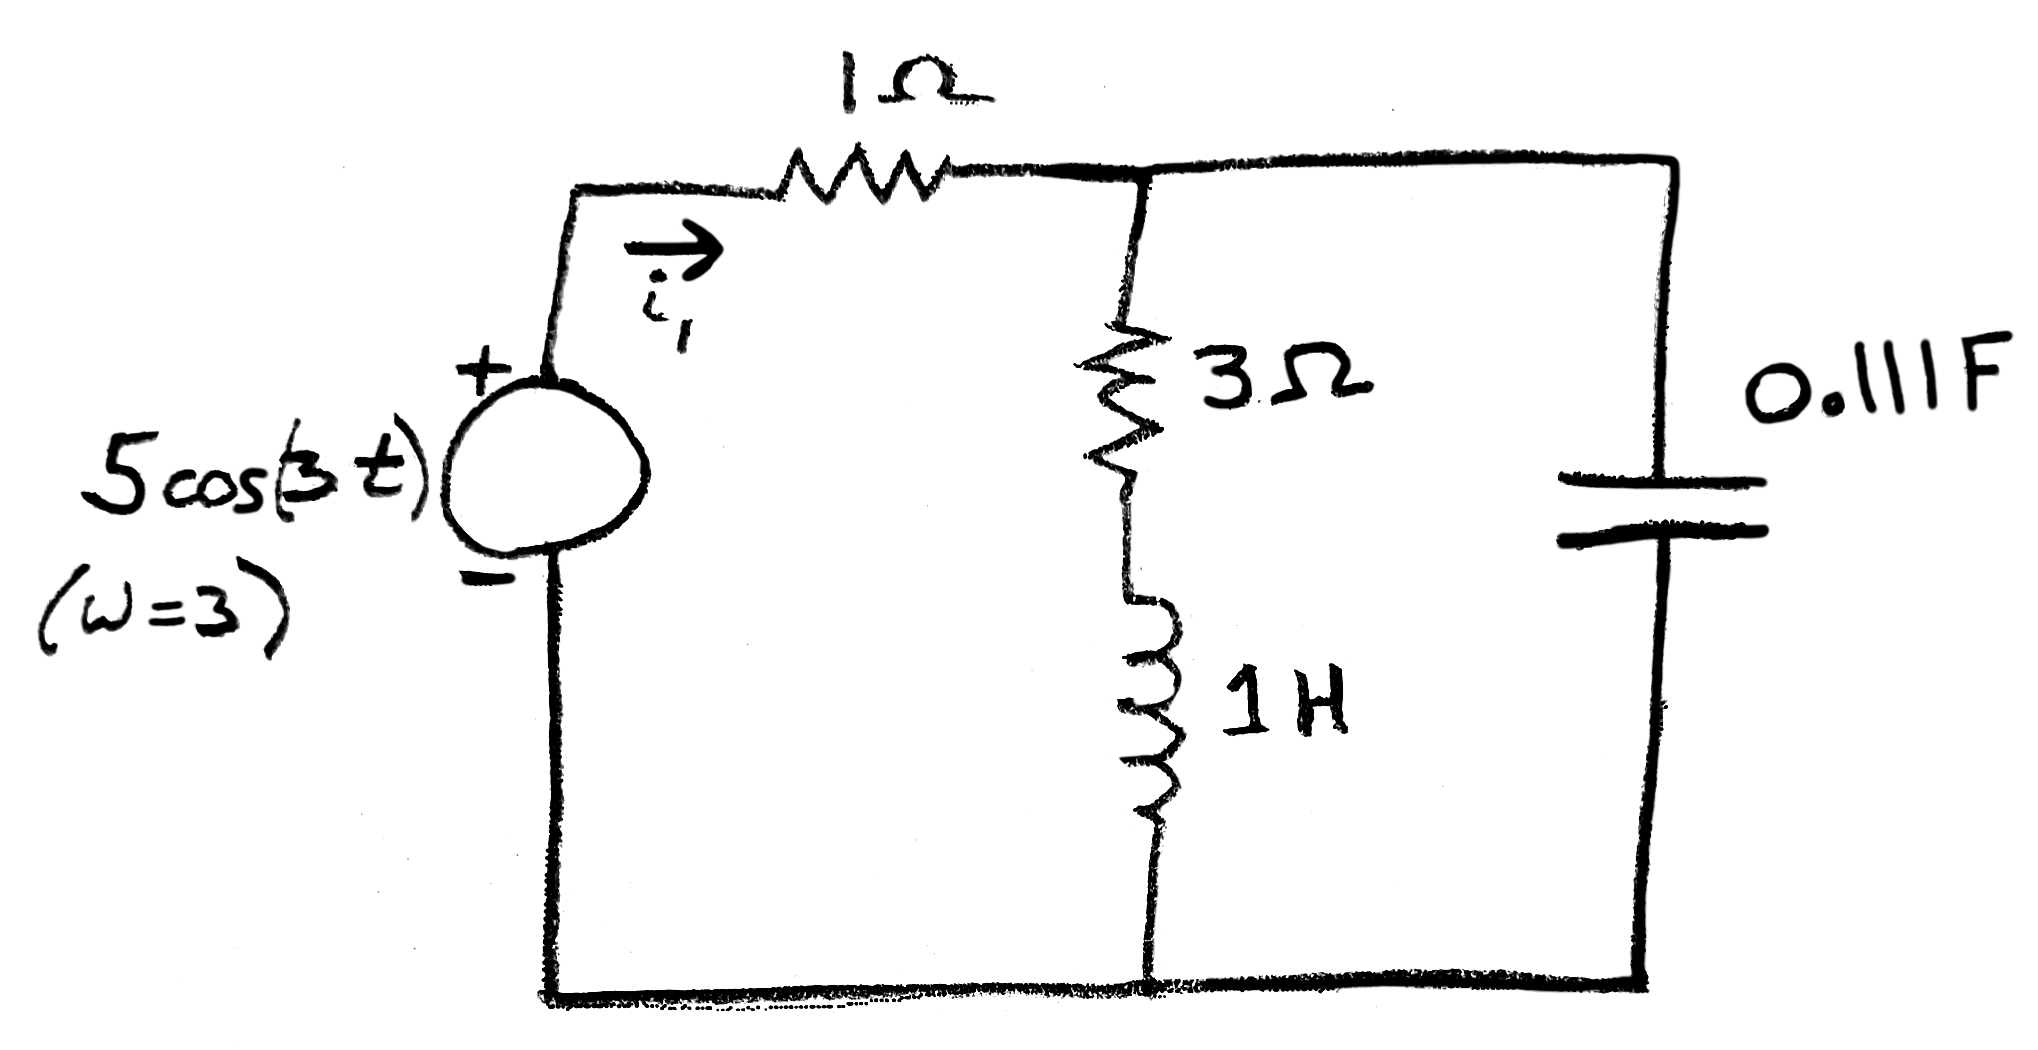
\includegraphics[width=0.5\textwidth]{figsChapt02/AM06622.png}

Q: Find the sinusoidal  steady state value of $i_1(t)$

A:

\[
\vec{I} = \frac{\vec{V}}  {Z} \; \to\; Z = \frac {\vec{V}}  {\vec{I}}
\]

Evaluate the impedances  in-place:

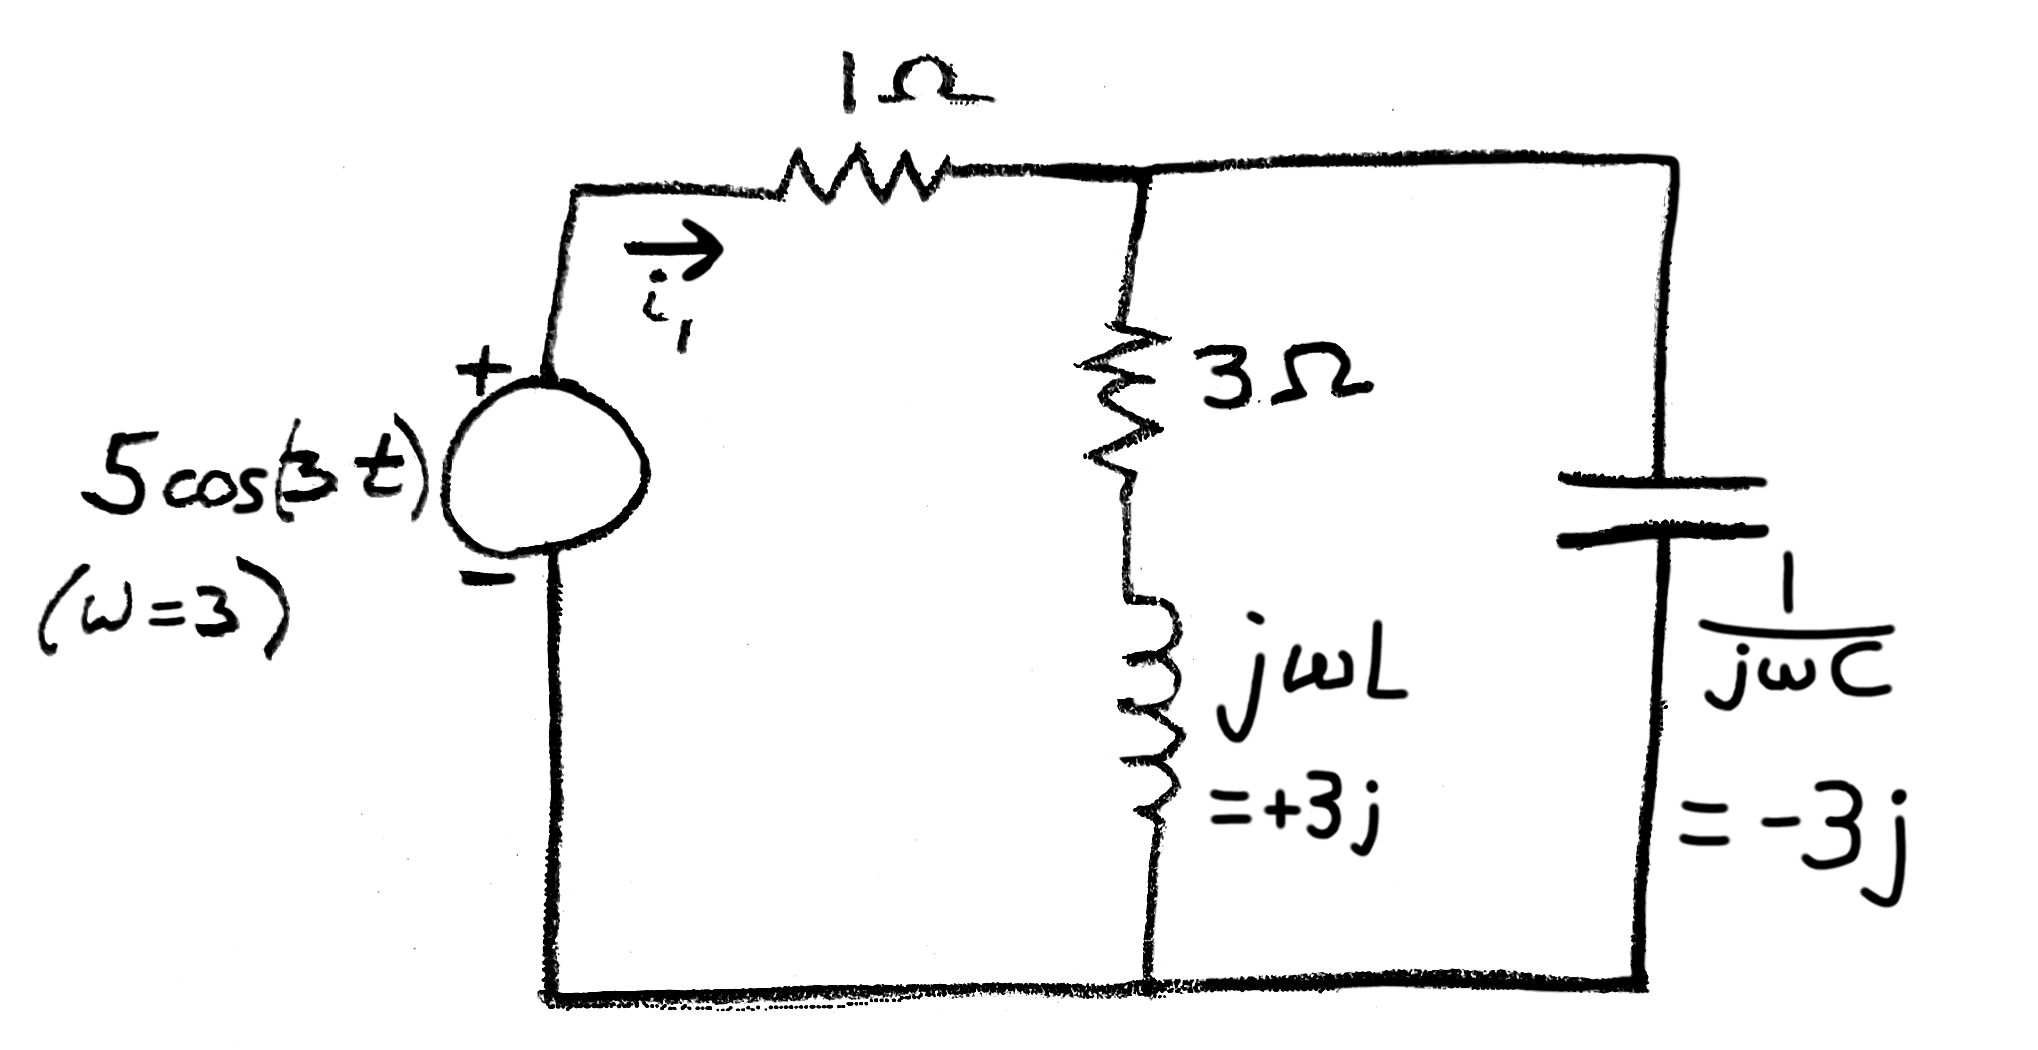
\includegraphics[width=0.5\textwidth]{figsChapt02/ME02007.png}

\[
Z =  1 + \frac{(3 + j3)(j3)}{3 + j3 + j3} = 1 + \frac{9 - 9j}{3} = 1 + 3 - 3j
= 4 - 3j
\]
(Net reactance is negative in other words, Capacitive)

\[
|Z| = \sqrt{16 + 9} = 5\Omega
\]


\[
\angle Z = \tan^{-1}\left(\frac{-3}{4}\right) = -37^\circ
\]

\[
\vec{I} = \frac{\vec{V}}{Z} = \frac{5e^{j0t}}{5e^{j37^\circ}} = 1e^{j37^\circ}
\]

\[\boxed{
i_L(t) = 1\cos(3t + 37^\circ)
}\]




Let's do one more KVL circuit example, just like Example \thechapter.\ref{firstPhasorCktKVL}, but with the addition of a capacitor.


\subsection{Series RLC  Circuit}\label{2ndPhasorCktKVL}

Now we add a capacitor to the simple series RL circuit:

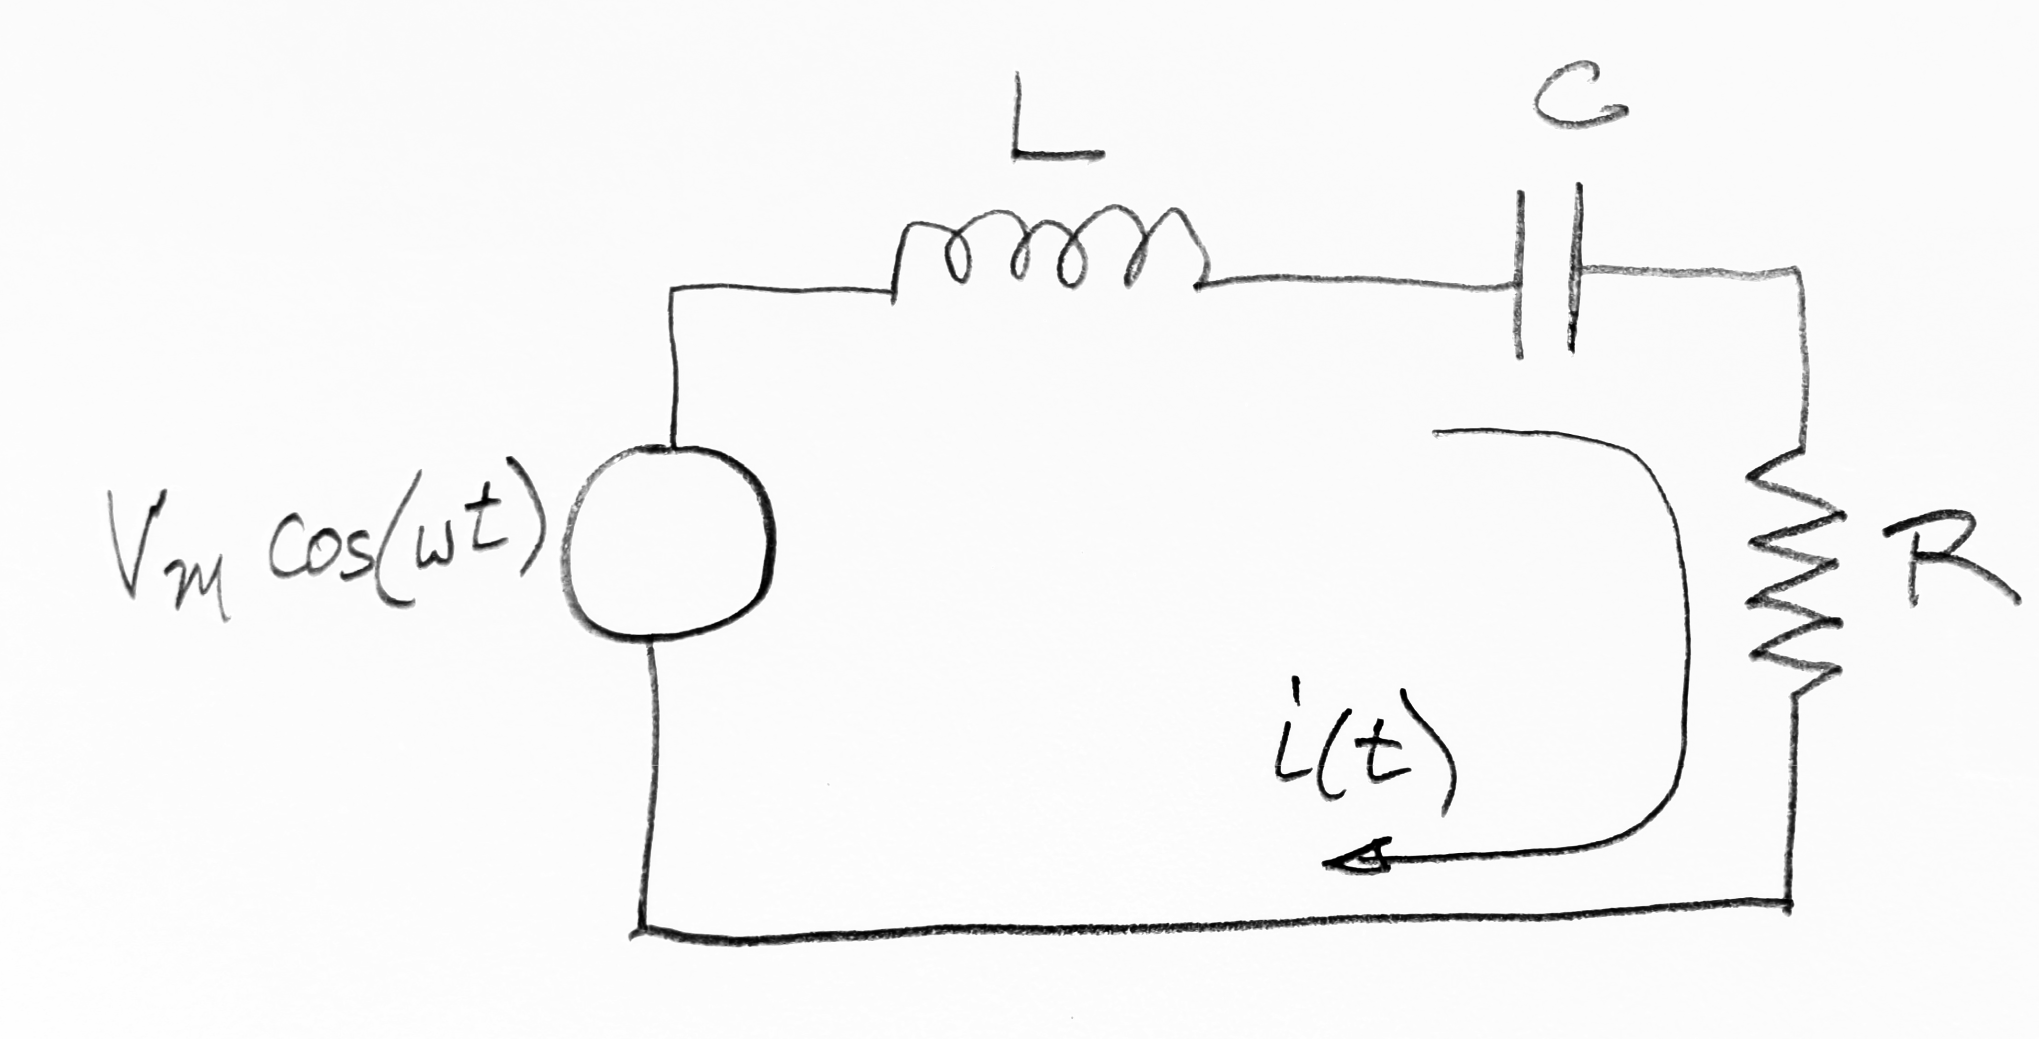
\includegraphics[width=0.5\textwidth]{figsChapt02/EL44497.png}

\begin{enumerate}
\item Using the definitions of capacitors, inductors, and resistors, and summing the  voltages around the loop:

\[
-V_M\cos(\omega t) + L\frac{di}{dt} + \frac {1}  { C}\int_0^t i\; dt + iR = 0
\]

\[
V_M\cos(\omega t) = L\frac{di}{dt}  + \frac {1}  {C}\int_0^t i\; dt + iR
\]

\item Consider input voltage to be the real part of two complex sinusoids:

\[
V_M\cos(\omega t) = \mathrm{Re}\{ \vec{V}e^{j\omega t} \}
\]
And we define
\[
i(t) = \mathrm{Re}\{ \vec{I}e^{j\omega t}  \}
\]
as the current phasor which is
unknown.

% \noindent $\{i \cdot \vec{V}, \vec{I}, V_0\}$

\item We plug the unknown current and voltage phasors into (1)

\[
\vec{V}e^{j\omega t} = j\omega L\vec{I}e^{j\omega t} + \frac {1}  {j\omega C}\vec{I}e^{j\omega t} +  R\vec{I}e^{j\omega t}
\]
(the leading $j\omega L$ term on the RHS comes from differentiating as in the original LODE and the $\frac {1}  {j\omega C}$
term comes from integration).


\item Next we factor out and cancel $e^{j\omega t}$ from all the terms:
\[
\vec{V} = j\omega L\vec{I} + \frac{1}{j\omega C} \vec I + R\vec{I}  = \vec{X}(R + j\omega L)
\]

As before we assume zero phase angle for input sinusoids so in this (common) case we have
\[
\vec{V} =V_Me^{j0} = V_M
\]


\end{enumerate}




Looking back at Section \ref{2ndPhasorCktKVL}, we get an abbreviated KVL analysis procedure.

First, we plugged in phasors for the sinusoidal quantities and
we got:

\[
\vec{V}e^{j\omega t} = j\omega L\vec{I}e^{j\omega t} + \frac{1}{j\omega C}\vec{I}e^{j\omega t} + \vec{I}Re^{j\omega t}
\]

Next we can  cancel out $e^{j\omega t}$ from every term giving

\[
\vec{V}  = j\omega L\vec{I}  + \frac{1}{j\omega C}\vec{I}  + \vec{I}R
\]
Now let's factor out $\vec{I}$ from all the RHS terms which gives

\[
\vec{V} = \vec{I} \left( j\omega L + \frac {1}  {j\omega C} +   R \right)
\]

The key observation is that we now are multiplying $\vec{I}$ by a single complex number to get $\vec{V}$
--- {\it instead of solving a differential equation!}


We call this complex quantity, in this circuit  $j\omega L + \frac {1}  {j\omega C} +   R $,
the Complex Impedance, or simply {\bf Impedance} of the circuit.
It is analogous to resistance, but   for sinusoidal
steady state problems.
So for this important class of AC problems, we can use a complex version of Ohm's law just
like DC circuits!


\begin{ExampleSmall}
Continue solving Example \ref{2ndPhasorCktKVL} to get the current phasor
$\vec{I}$.

\paragraph{Solution}

\[
\vec{I} = \frac {\vec{V}}  {j\omega L + \frac {1}  {j\omega C} +   R} =
\frac {V_M}  {j\omega L + \frac {1}  {j\omega C} +   R}
\]

($\vec{V} =V_M$
because we usually choose the source voltage to have zero phase,
$\vec{V} = V_Me^{j\omega t + 0}$
).

Simplifying we multiply by $j/j$:
\[
= \frac {jV_M}  {-\omega L + \frac {1}  {\omega C} + jR }
\]
\[
\vec{I} = \frac {jV_M}  {(\frac {1}  {\omega C}-\omega L) + Rj} = \frac {V_M}  {R-j(\frac {1}  {\omega C}-\omega L)}
\]
dividing complex numbers is easier in polar form so
\[
|R-j(\frac {1}  {\omega C}-\omega L)| = \sqrt{R^2+ \left (\frac {1}  {\omega C}-\omega L\right )^2}
\]
\[
\angle{R-j\left (\frac {1}  {\omega C}-\omega L\right )}  = -\tan^{-1}\left ( \frac {\frac {1}  {\omega C}-\omega L}  {R} \right )
\]
\[
\vec{I} = V_M \frac {1}  {\sqrt{R^2+(\frac {1}  {\omega C}-\omega L)^2}}e^{j\phi},\;\; \phi =  -\tan^{-1}\left ( \frac {\frac {1}  {\omega C}-\omega L}  {R} \right )
\]
\end{ExampleSmall}



\subsection{Effects of Frequency on Reactance}

Looking again at the impedance of the circuit in the previous subsection, we have
\[
Z_{tot}  =  j\omega L + \frac {1}  {j\omega C} +   R
\]

Diagramming the impedance components as we did in section \ref{seriesRLckt}, we see that
the inductive reactance and the capacitive reactance are always in opposition.  Repeating
the diagram:

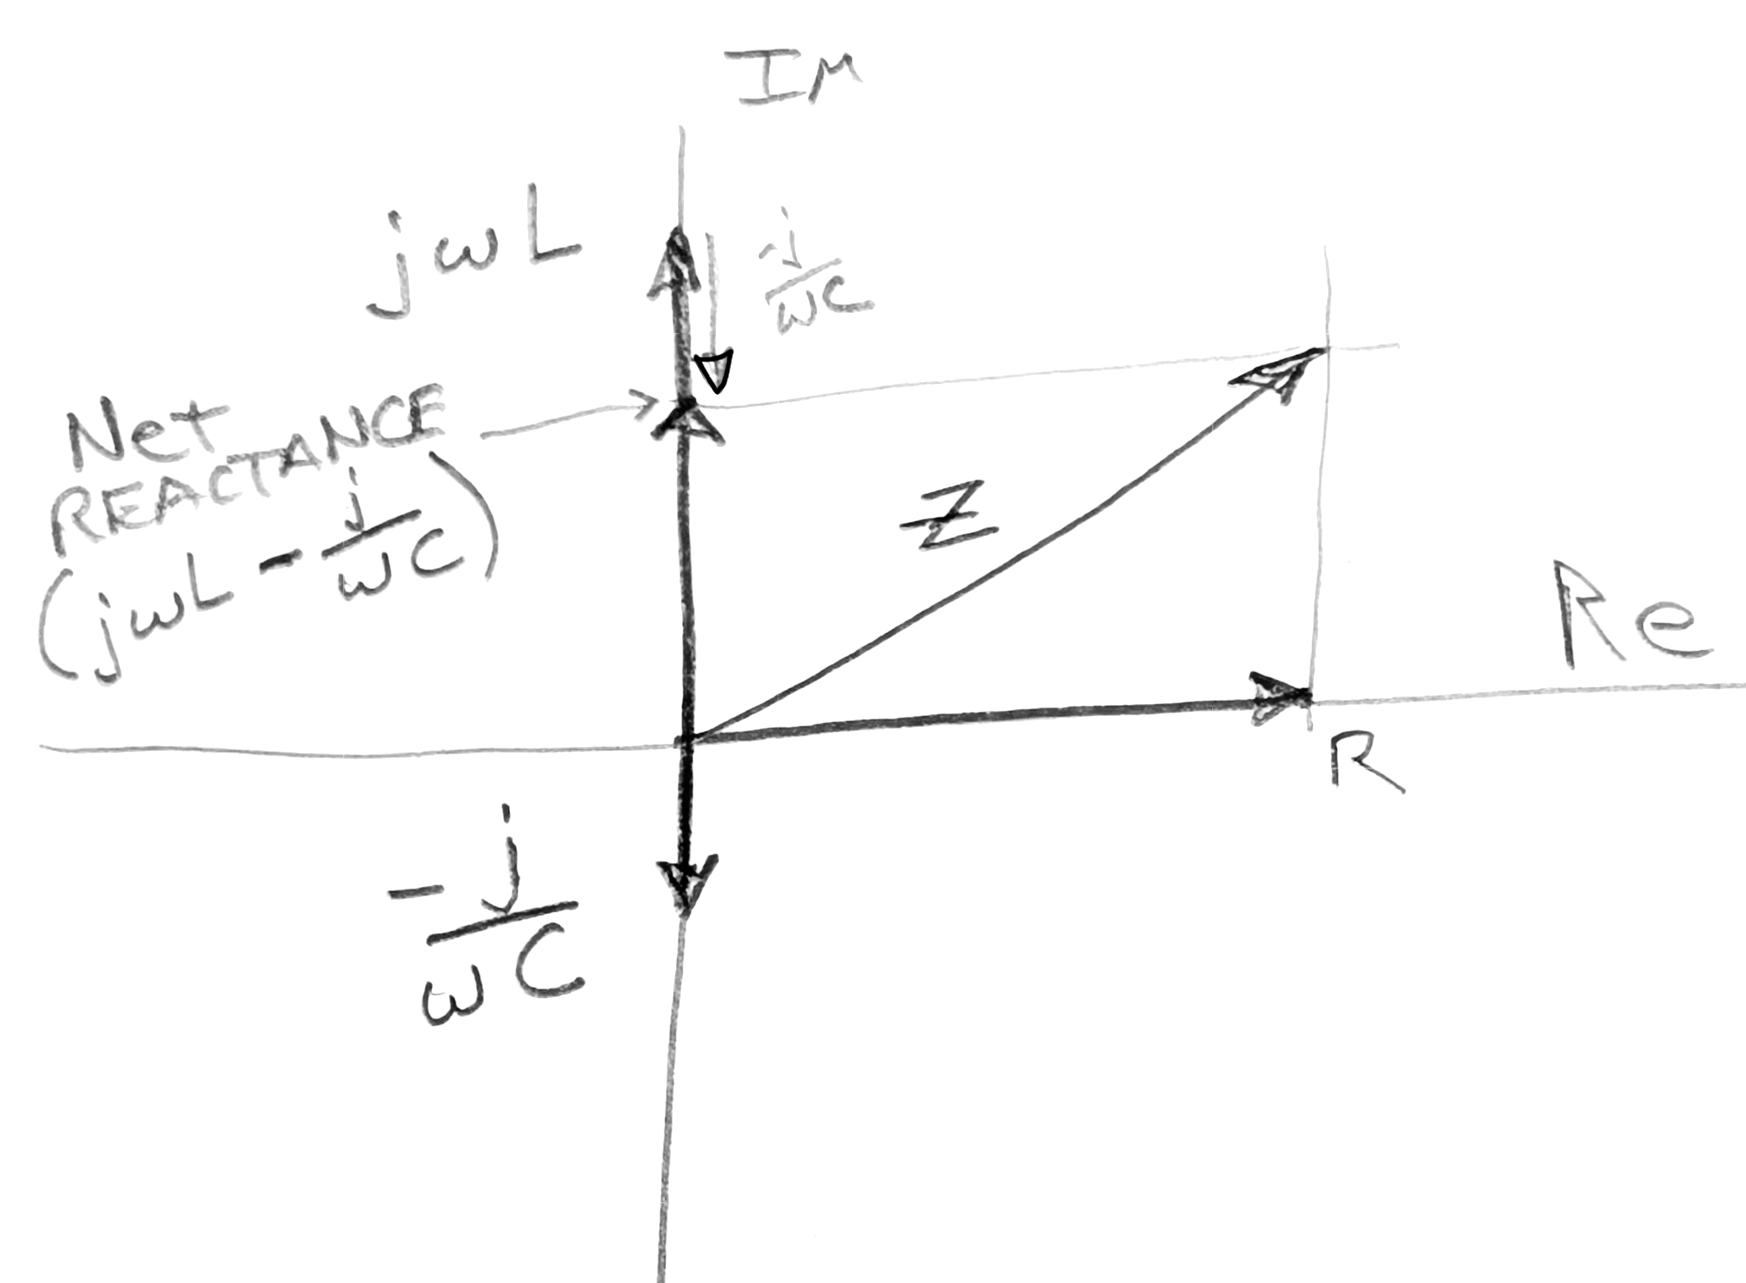
\includegraphics[width=0.5\textwidth]{figsChapt02/HF41781.png}

Notice that $\omega$ appears inverted in the capacitive reactance, so the magnitude of these
two components varies inversely with frequency.

Let's compute the net reactance for a series of frequencies. Where
\[
Z_{2}  =  j\omega L + \frac {1}  {j\omega C}
\]
(only the imaginary components of $Z_{tot}$).
Of course we have to assume some component values:

eg.
\[
L = 1\text{mH},\; C = 1000\mu\text{F}
\]

Writing a tiny python script to
chart the reactance ($X$) at several frequencies we get:

\begin{verbatim}import numpy as np
L = 0.001
C = 1.0E-3
j = 0.0+1.0j
ww = [10, 100, 5E2, 1000, 5e3, 1.0e4, 1.0e5]
print(' w             X')
for w in ww:
   X = j*w*L + 1.0/(j*w*C)
   print(f'{w:.2e} {np.imag(X):>8.2f}')

 w             X
1.00e+01   -99.99
1.00e+02    -9.90
5.00e+02    -1.50
1.00e+03     0.00
5.00e+03     4.80
1.00e+04     9.90
1.00e+05    99.99
\end{verbatim}

For these component values the net reactance is negative (capacitive) below 1000 rad/sec
and positive (inductive) above 1000 rad/sec.

Let's take this one step further and evaluate the whole impedance (putting $R$ back in the picture).
We have to specify the resistance:
\[
R = 10\Omega
\]
Now the script changes to

\begin{verbatim}import numpy as np
L = 0.001
C = 1.0E-3
R = 10
j = 0.0+1.0j
ww = [ 10, 100, 5E2, 1000, 5e3, 1.0e4, 1.0e5]
print(' w             X      |Z|        /_Z (deg)       Z')
for w in ww:
   X = j*w*L + 1.0/(j*w*C)
   Z =  R + j*w*L + 1.0/(j*w*C)
   ang = 360 * np.angle(Z)/(2*np.pi)
   print(f'{w:.2e} {np.imag(X):>8.2f}  {np.abs(Z):>8.2f}  {ang:>8.2f}
            {np.real(Z):8.2f} + {np.imag(Z):8.2f}j' )

 w             X      |Z|        /_Z (deg)       Z
1.00e+01   -99.99    100.49    -84.29      10.00 +   -99.99j
1.00e+02    -9.90     14.07    -44.71      10.00 +    -9.90j
5.00e+02    -1.50     10.11     -8.53      10.00 +    -1.50j
1.00e+03     0.00     10.00      0.00      10.00 +     0.00j
5.00e+03     4.80     11.09     25.64      10.00 +     4.80j
1.00e+04     9.90     14.07     44.71      10.00 +     9.90j
1.00e+05    99.99    100.49     84.29      10.00 +    99.99j
\end{verbatim}

Note how the angle changes to almost $\pm90^\circ$ as the magnitude of the reactance dominates $R$.

\section{Voltage and Current Dividers with Impedances}
Just as with parallel and series combinations, voltage dividers work in a very similar way with impedances.


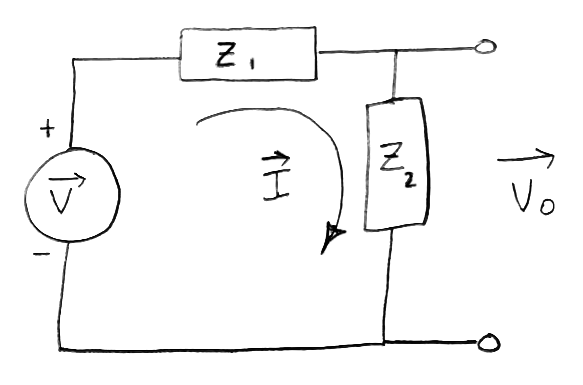
\includegraphics[width=0.35\textwidth]{figsChapt02/CT64010.png}

\[
\vec{V} = \vec{I}(Z_1+Z_2)
\]
\[
\vec{V}_o = \vec{I} Z_2
\]
\[
\frac {\vec{V}_0 } {\vec{V}} = \frac {Z_1}  {Z_1+Z_2}
\]

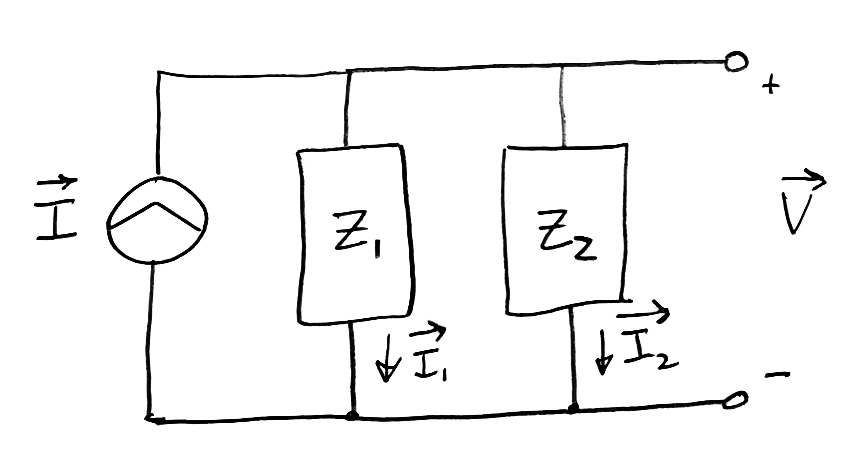
\includegraphics[width=0.35\textwidth]{figsChapt02/LE10258.png}

For Current Dividers, we can leverage admittances, which like conductances, make it somewhat simpler.
\[
\vec{I} = \vec{V}(Y_1+Y_2) = \vec{V}(\frac {1}  {Z_1} + \frac {1}  {Z_2}  )
\]

\[
\vec{I}_1 = \vec{V} Y_{1}
\]

\[
\frac {\vec{I}_1}  {\vec I_1+\vec I_2} = \frac {\vec V Y_1}  {\vec V (Y_1+Y_2)}
\]

\[
\frac {\vec{I}_1}  {\vec I_1+\vec I_2} = \frac {\frac {1}  {Z_1}}  {\frac {1}  {Z_1}+\frac {1}  {Z_2}} =
\frac {1}  {1+\frac {Z_1}  {Z_2} } = \frac {Z_2} {Z_1+Z_2}
\]

And for three parallel impedances:


\[
\frac {\vec{I}_1}   {\vec I_1+\vec I_2+\vec I_3} = \frac {Y_1}  {Y_1+Y_2+Y_3} =
\frac {\frac {1}  {Z_1}}  {\frac {1}  {Z_1}+\frac {1}  {Z_2}+\frac {1}  {Z_3}} =
\frac {Z_2 Z_3}  {Z_2 Z_3 + Z_1 Z_3+ Z_1 Z_2}
\]

\section{Thevenin and Norton Equivalents with Impedances}

Consider a ``black box'' -- a circuit with (in this case) two terminals, but we can't see what's inside it.   Or, we can see
a very complex network of sources and impedances inside and we want a simpler {\it but equivalent} version.

\begin{center}
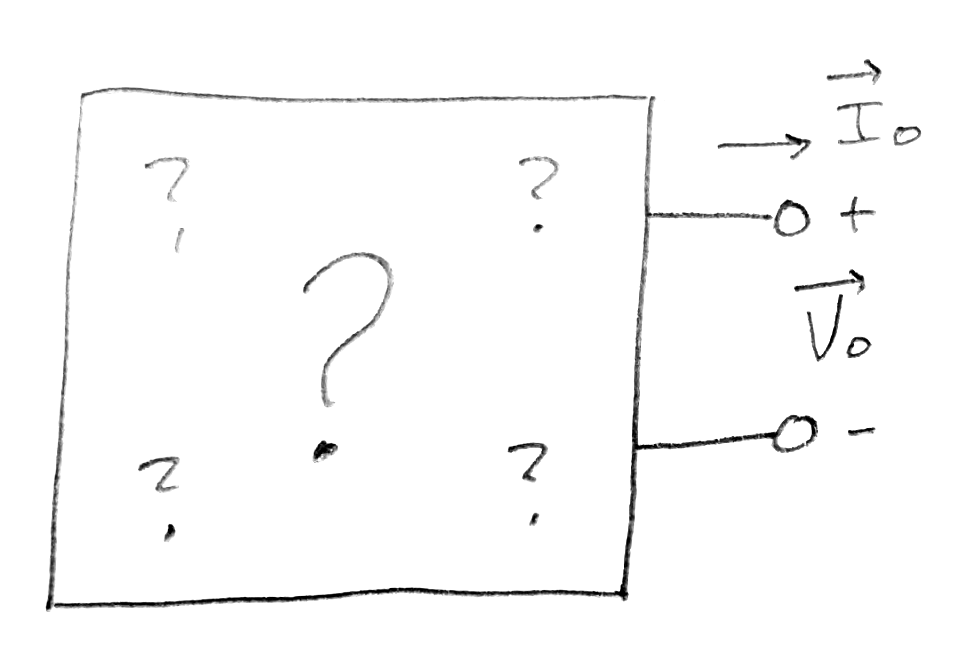
\includegraphics[width=0.25\textwidth]{figsChapt02/AJ40622.png}
\end{center}

With phasors and impedances we can redo the DC concepts of Theven and Norton equivalent circuits as follows:

\vspace{0.2in}
\noindent
\hspace{0.5in}Thevenin \hspace{2.0in} Norton

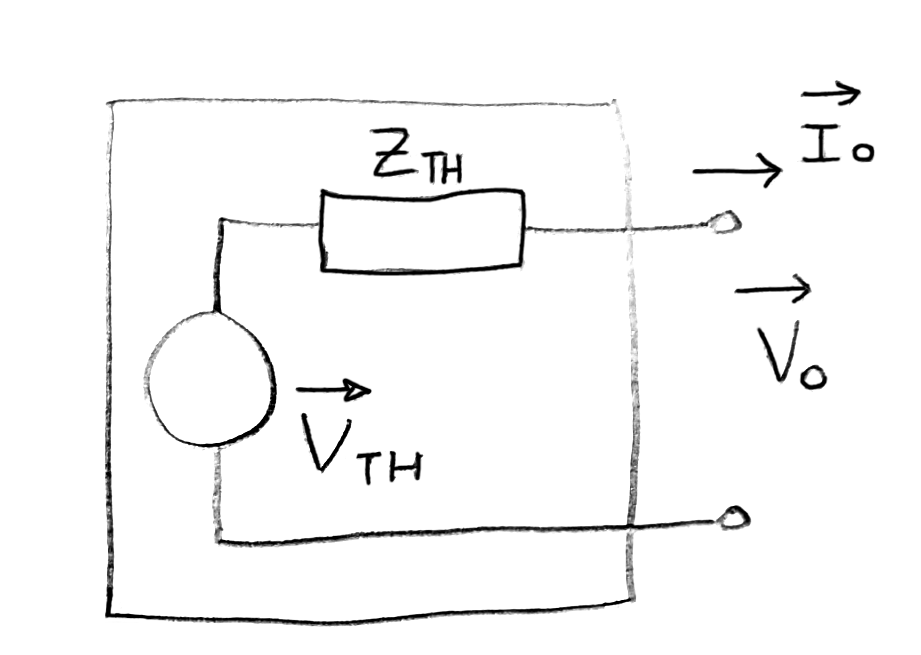
\includegraphics[width=0.25\textwidth]{figsChapt02/GT93824.png}\hspace{1.0in}
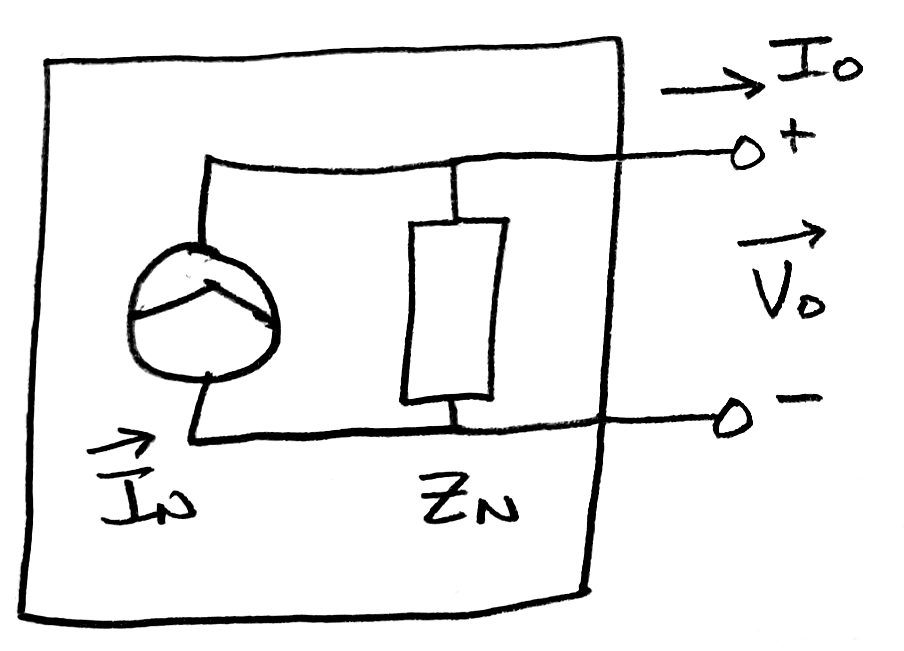
\includegraphics[width=0.25\textwidth]{figsChapt02/UN79919.png}

\vspace{0.2in}
We have a KVL equation to define the Thevenin equivalent:
\[
-\vec{V}_{TH} + \vec{I}_o Z_{TH} + \vec{V}_o = 0
\]

\[\boxed{
\vec{V}_{TH} = \left . \vec{V}_o \right |_{\vec{I}_o=0}
}
\]
(where $\vec{I}_o=0$ is the same as an open circuit of the output.)
\[\boxed{
Z_{TH} = \left . \frac
        { \vec{V}_{TH}}
        { \vec{I}_o}
        \right |_{\vec{V}_o=0  }
  }
\]
(where $\vec{V}_o=0$ is the same as a short circuit of the output.)

We also have a KCL equation to define the Norton equivalent:
\[
\vec{I}_N = \left . \vec{I}_o \right|_{\vec{V}_o=0}
\]
\[\boxed{
\vec{I}_N = \left . \vec{I}_o \right|_{\vec{V}_o=0}
}
\]
\[\boxed{
Z_N = \left . \frac {\vec{V}_o}  {\vec{I}_N} \right | _{\vec{I}_o = 0} }
\]


Note that as in the DC case, $Z_{TH} =Z_N$.


\subsection{Theven  Example with Phasors}
\begin{Example}

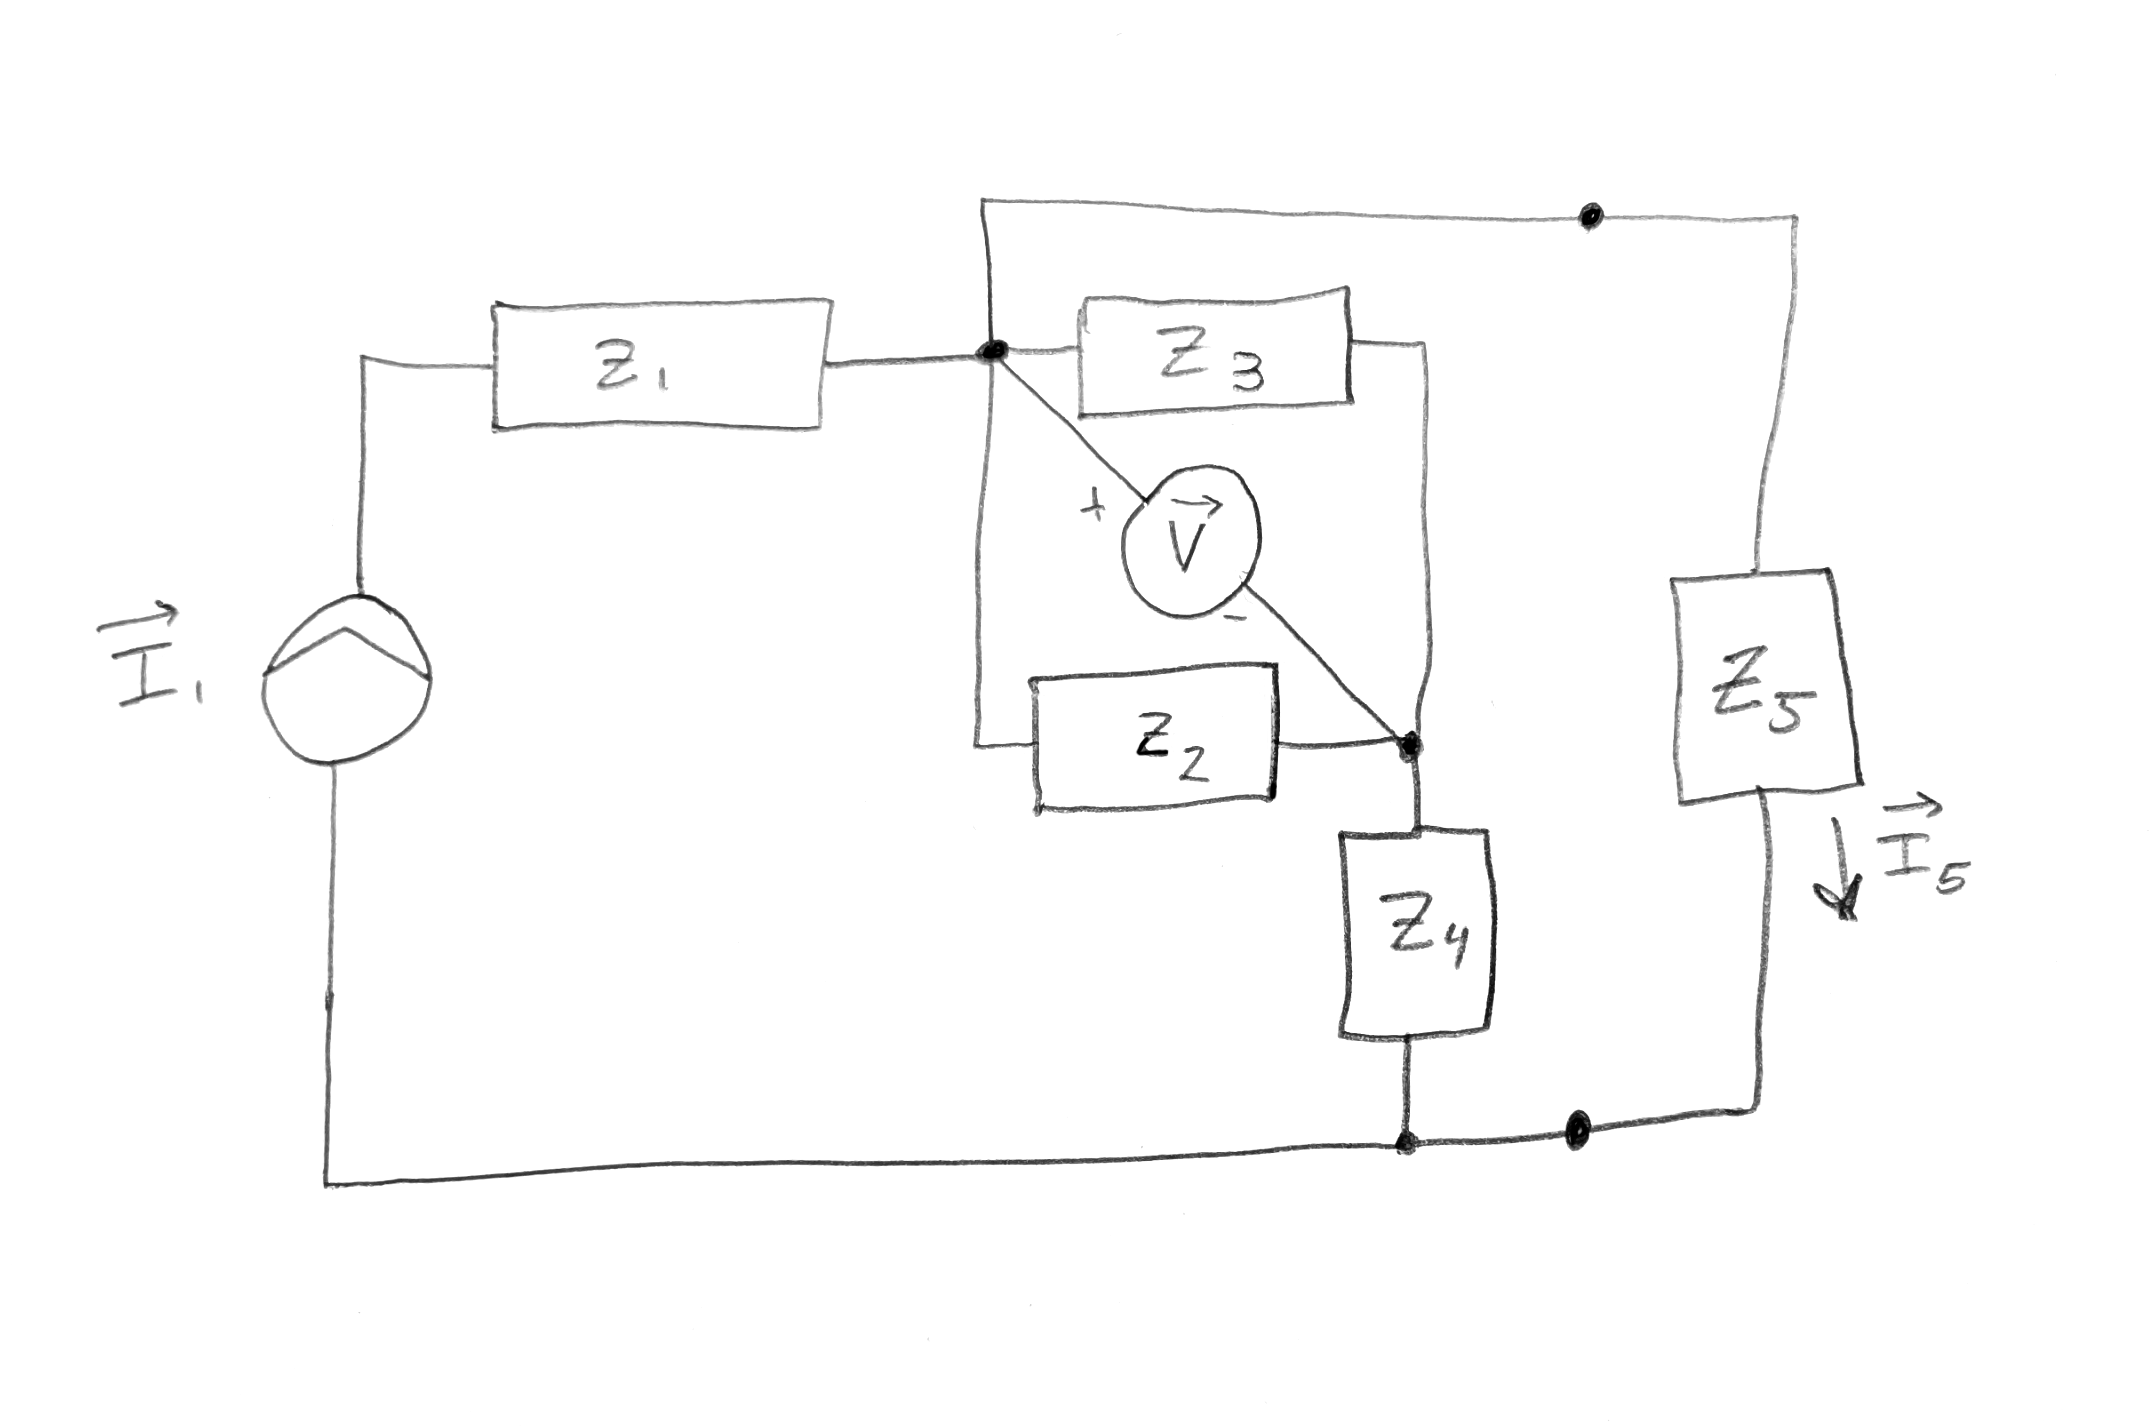
\includegraphics[width=125mm]{figsChapt02/KS52020.png}

\paragraph{Problem:} We need to find $\vec I_5$ in the above circuit. We {\it could}
write node and mesh equations, solve them, and get $\vec I_5$.

{\bf Warning:}  This is a tricky circuit!
Do not get too frustrated on this problem, give it a try and then read through the analysis
below if you get stuck!


\paragraph{Solution:}
We'll try a
Thevenin  equivalent circuit as follows.


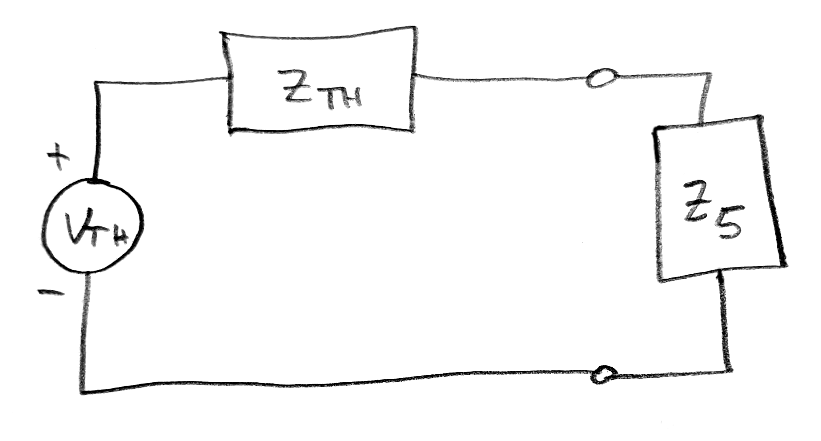
\includegraphics[width=66mm]{figsChapt02/DE22052.png}

If we can get all the stuff to the left of $Z_5$ into the Thevenin equivalent,
the problem will be simple, specifically,

\[
\vec I_5 = \frac {\vec V_{TH}}  {Z_{TH}+Z_5}
\]

We learned above that
\[
\vec{V}_{TH} = \left . \vec{V}_o \right |_{\vec{I}_o=0}
\quad
\text{and}
\quad
Z_{TH} = \left . \frac
        { \vec{V}_{TH}}
        { \vec{I}_{SS}}
        \right |_{\vec{V}_o=0  }
\]
\end{Example}
\begin{ExampleCont}

The tricky part of the problem is that we have impedance in series with a current source
and two impedance in parallel with a voltage source.  Consider these cases below:


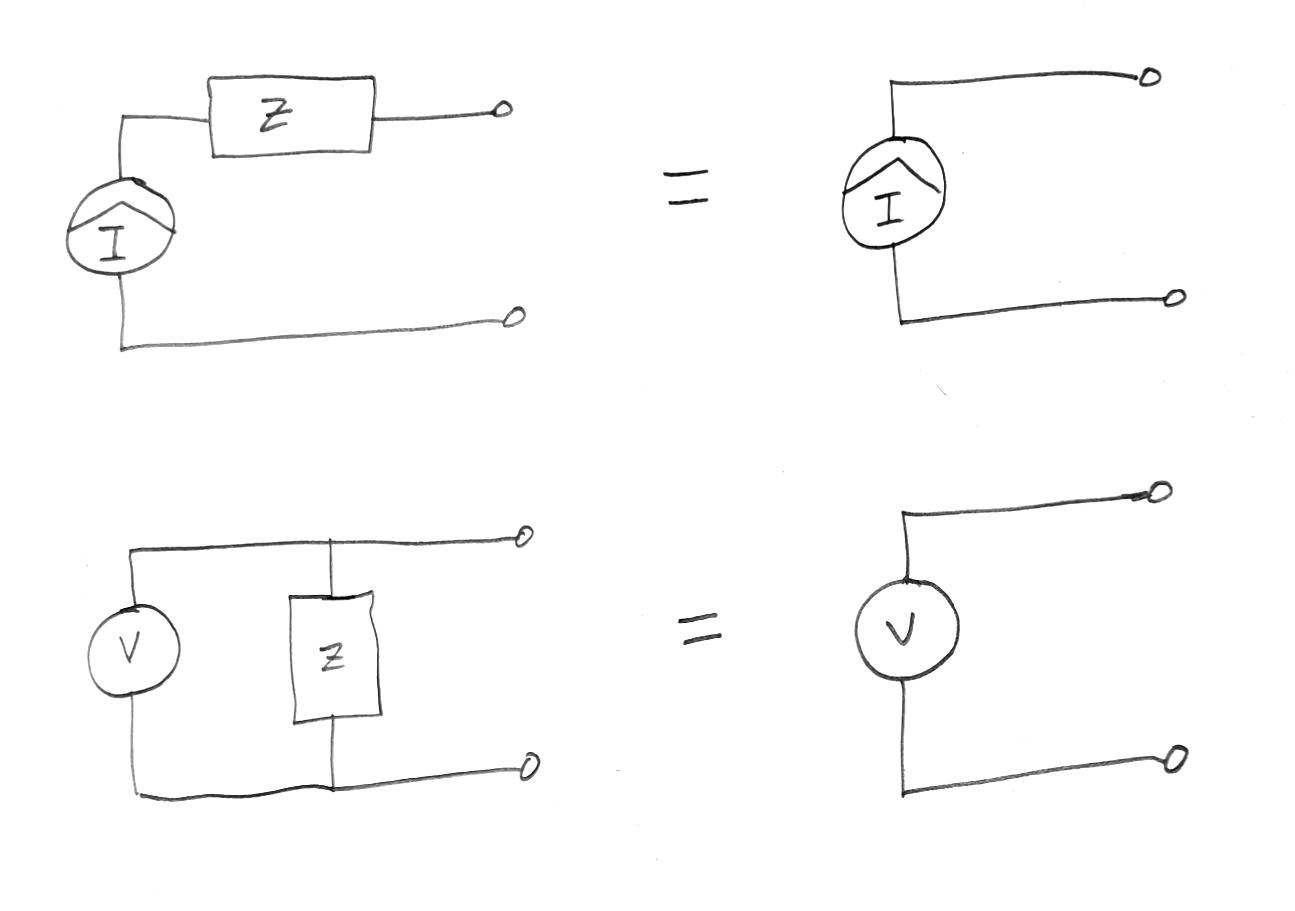
\includegraphics[width=100mm]{figsChapt02/SA35824.png}

Notice that in both cases, the impedance makes no difference in terms of
the output of the circuit for any possible load connection!  That's because the sources
are ``ideal''.   We can apply this to simplify the circuit quite a bit as follows:

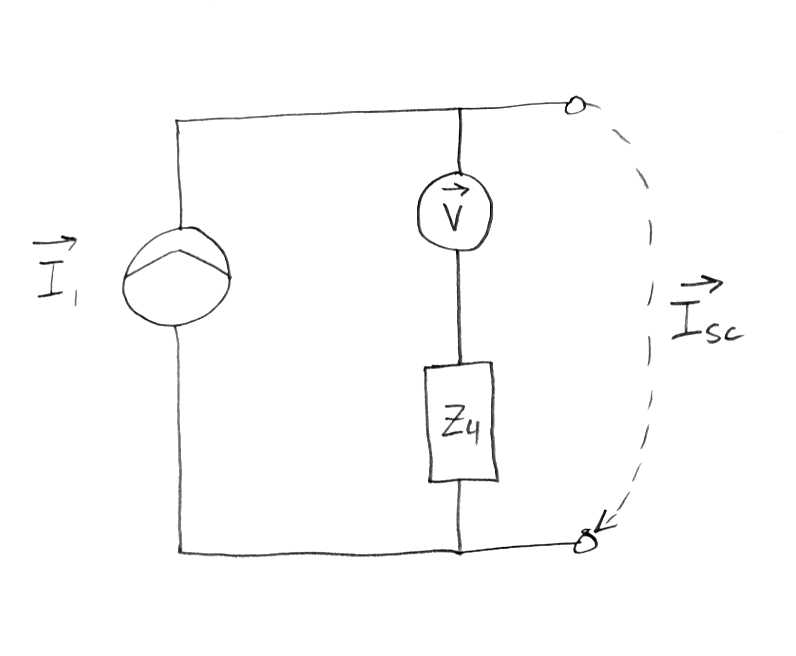
\includegraphics[width=100mm]{figsChapt02/HL67285.png}


First, working on $\vec V_{TH} = \vec V_{OC}$ by going around the loop:
\[ \boxed{
V_{TH} = \vec I_1Z_4+\vec V
}
\]

\end{ExampleCont}
\begin{ExampleCont}

Now, adding a short circuit to the output, we look at $\vec I_{SC}$.   Here we take a superposition approach:

1)  Set $\vec I_1 = 0$ giving
\[
\vec I_{SC1} = \frac {\vec V}{Z_4}
\]

2) Set $\vec V = 0$ giving
\[
\vec I_{SC2} = \vec I_1
\]

3) Finally,
\[
\vec I_{SC} = \vec I_{SC1} + \vec I_{SC2} = \vec I_1 +  \frac {\vec V}{Z_4}
\]

Now we get $Z_{TH}$ by
\[
Z_{TH} = \frac {\vec V_{OC}} {\vec I_{SC}} = \frac  {\vec I_1Z_4+\vec V}  {\vec I_1 +  \frac {\vec V}{Z_4}}
\]
\[
Z_{TH} = Z_4  \frac  {\vec I_1Z_4+\vec V}  {\vec I_1Z_4 +  \vec V}
\]
\[\boxed{Z_{TH} = Z_4  }
\]


Finally we work out the requested answer, $\vec I_5$:

\[
\vec I_5 = \frac {\vec V_{TH}} {Z_{TH} + Z_5}
\]
\[\boxed{
\vec I_5 =  \frac{\vec I_1Z_4 + \vec V}  {Z_4+Z_5}   }
\]

\end{ExampleCont}
%


**************************************************  BH Stopped here (10/8/25)




\section{Simultaneous Equations for Multiple Loops}

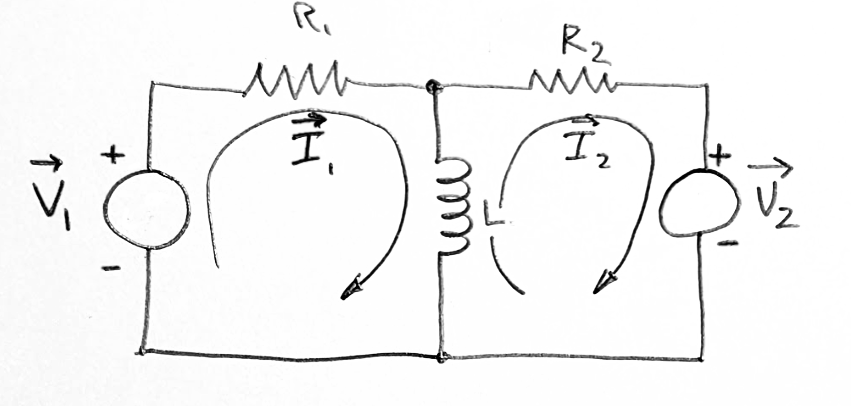
\includegraphics[width=0.33\textwidth]{figsChapt02/KT62219.png}


\subsection*{Problem:}
Find $\vec{I}_1$ and $\vec{I}_2$

\subsection*{Solution:}
Step 1) Write the 2 mesh (loop) equations

\[-\vec{V}_1 + \vec{I}_1 R_1 + j\omega L(\vec{I}_1 - \vec{I}_2) = 0\]

\[\vec V_2 + \vec{I}_2 R_2 + j\omega L(\vec{I}_2 - \vec{I}_1) = 0\]

Step 2) Organize by circuit variables

\[(R_1 + j\omega L)\vec{I}_1 - j\omega L\vec{I}_2 = \vec V_1\]

\[-j\omega L\vec{I}_1 + (R_2 + j\omega L)\vec{I}_2 = -\vec V_2\]

3) Solve these 2 simultaneous equations
   \begin{enumerate}
   \item by substitution (N $\leq$ 3)
   \item by Matrices/Cramer's Rule (N $\leq$ 4)
   \item by Computer (N $>$ 2)($\geq 2$ ?)
   \end{enumerate}

\section*{Note on Matrix Construction}

Factor 2 into:

\[
{Z}{\vec{I}} = \vec{V}\]

e.g.
\[\begin{bmatrix}
R_1 + j\omega L & -j\omega L \\
-j\omega L & R_2 + j\omega L
\end{bmatrix}
\begin{bmatrix}
\vec{I}_1 \\
\vec{I}_2
\end{bmatrix}
=
\begin{bmatrix}
\vec \vec V_1 \\
-\vec \vec V_2
\end{bmatrix}\]

\subsection*{Notes:}
\begin{itemize}
\item $Z_{11}, Z_{22}, Z_{33} \rightarrow$ the diagonal elements, are the sum of all impedances in loop i.
\item For simple impedance like $ Z_{12} $ in other words $Z_{ij}$, the off diagonal
elments are the (negative of the) impedances which couple two loops (i.e. loop 1 to loop 2).
\item  The lower diagonal same as upper  diagonal, e.g. $Z_{13} = Z_{31}$
\end{itemize}

\textbf{The above are ways to check for a correct impedance matrix.}

\paragraph{Solving by Substitution}

From the matrix form above, let $Z_{21}$ be the term at row 2 col 1 of Z

% n.b. $Z_{12} = Z_{21} = -j\omega L$, Row 2, Col 1

\[\vec{I}_1 = \frac{\vec V_1 - Z_{12}\vec{I}_2}{Z_{11}}\]

\[\frac{Z_{21}}{Z_{11}} \vec{V}_1 - \frac{Z_{21}Z_{12}}{Z_{11}}\vec{I}_2 + Z_{22}\vec{I}_2 = -\vec{V}_2\]

\[\vec{I}_2\left(Z_{22} - \frac{Z_{21}Z_{12}}{Z_{11}}\right) = -\frac{Z_{21}}{Z_{11}}\vec V_1 - \vec V_2\]

\[\vec{I}_2 = \frac{-\frac{Z_{21}}{Z_{11}}\vec V_1 - \vec V_2}{Z_{22} - \frac{Z_{21}Z_{12}}{Z_{11}}} = \frac{-Z_{21}\vec V_1 - Z_{11}\vec V_2}{Z_{11}Z_{22} - Z_{21}Z_{12}}\]

\[\vec{I}_1 = \frac{1}{Z_{11}}\vec V_1 - \frac{Z_{12}}{Z_{11}} \frac{-Z_{21}\vec V_1 - Z_{11}\vec V_2}{Z_{11}Z_{22} - Z_{21}Z_{12}}\]

\[= \frac{1}{Z_{11}}\vec V_1 + \frac{Z_{12}Z_{21}\vec V_1 + Z_{12}Z_{11}\vec V_2}{Z_{11}(Z_{11}Z_{22} - Z_{21}Z_{12})} + \frac{Z_{12} \vec V_2}{Z_{11}Z_{22} - Z_{21}Z_{12}}\]

\[= \vec V_1 \frac{(Z_{11}Z_{22} - Z_{21}Z_{12}) + Z_{12}Z_{21}}{Z_{11}(Z_{11}Z_{22} - Z_{21}Z_{12})} + \vec V_2 \frac{Z_{12}}{Z_{11}Z_{22} - Z_{21}Z_{12}}\]

\[\vec{I}_1 = \frac{Z_{22}\vec V_1 + Z_{12}\vec V_2}{Z_{11}Z_{22} - Z_{21}Z_{12}}\]

\subsection{More Complicated Network Example}


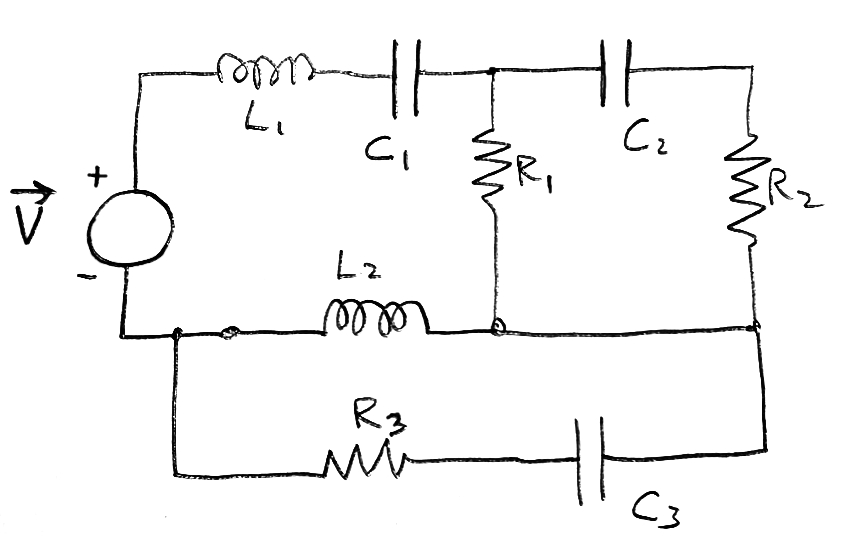
\includegraphics[width=0.6\textwidth]{figsChapt02/EU33724.png} % 10/1/25s

\begin{align*}
L1 &= 2.5 H\\
L2 &= 2.5 H\\
C1 = C2 &= 1/40 F\\
C3 &= 1/80 F\\
R1 = R1 &= 10\Omega\\
R3 &= 5\Omega
\end{align*}

\paragraph{Problem:} Solve the entire circuit to find (for example, $V_0$, $\vec{I}_3$, R)
\vspace{0.2in}

Step 0)  Compute the impedance of each component and re-label the schematic:


\[\omega = 4, L = 2.5H
\]
\[j\omega L =  j10
\]
\[4L = \frac{1}{4C} = 10
\]
\[L = 2.5
\]
\[
C = \frac{1}{40}
\]
\[
\frac{1}{j\omega C} = -j10
\]


Now we place these impedances onto the schematic, and add current loops:

\vspace{0.2in}
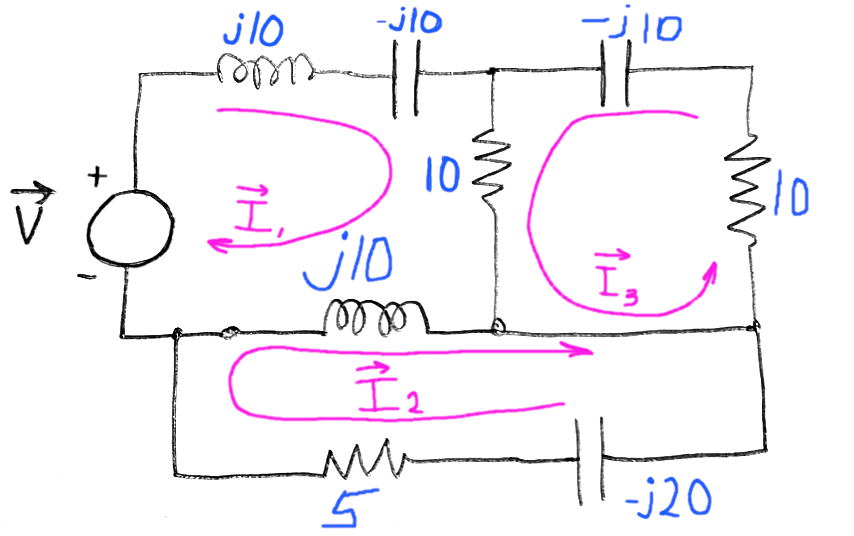
\includegraphics[width=0.6\textwidth]{figsChapt02/LK37610.png} % 10/1/25s

{\bf Note: }   The usual best practice is to make all your current loops either
clockwise or counter clockwise.   However this not a strict requirement.  Because
$\vec I_3 $ is different from the other two, we will just have to watch our signs
a little more carefully below!


\vspace{0.2in}
1) Write 3 Mesh equations
%(N.B.: $j\omega L = j4(2.5),\;\; \frac{1}{j\omega C} = -\frac{j40}{4}$)

  \[
  -V + (j10 - j10)\vec{I}_1 + (\vec I_1 + \vec{I}_3)10 + (\vec{I}_1 - \vec{I}_2)j10 = 0
  \]

  \[
  -j20\vec{I}_2 + 5\vec{I}_2 + j10(\vec{I}_2 - \vec{I}_1) = 0
  \]

  \[
 -j10\vec{I}_3 + 10(\vec{I}_3 + \vec{I}_1) + \vec{I}_3 10 = 0
  \]

2) Arrange:
  \[
  (10 + j10)\vec{I}_1 + (-j10)\vec{I}_2 + (10)\vec{I}_3 = V
  \]
  \[
  (-j10)\vec{I}_1 + (5 - j10)\vec{I}_2 + (0)\vec{I}_3 = 0
  \]
  \[
  (10)\vec{I}_1 + (0)\vec{I}_2 + (20 - j10)\vec{I}_3 = 0
  \]

3) Solve:
\[Z = \begin{bmatrix}
10 + j10 & -j10 & 10 \\
-j10 & 5 - j10 & 0 \\
10 & 0 & 20 - j10
\end{bmatrix}\]

Symmetry check: {\bf PASS}

\vspace{0.2in}
This result gives us the final matrix equation:

\[
Z\vec{I} = \vec{V}
\]

We can, for example, now solve for the currents by
\[
\vec I = (Z^{-1}) \vec V
\]
(using python for example which makes easy work of inverting the 3x3 matrix.)

\paragraph{Alternate method}

Let's get Z even more directly:

Diagonal: $Z_{ii}$ are sums of impedances around each loop:
\[Z_{11} = j10 + (-j10) + 10 + j10 = j10 + j10\]
\[Z_{22} = -j20 + 5 + j10 = 5 - j10\]
\[Z_{23} = 10 - j10 + 10 = 20 - j10\]

Off Diagonal: $Z_{ij}$ = impedance common to both loops $i$ and $j$ (negating the term
if the two current loops go in opposite directions.)
% \& j (- sign (j))wrt $\vec{I}_i$ and $\vec{I}_j$

\[
Z_{12} = j10 -1
\]
$\vec{I}_1, \vec{I}_2$ have opposite signs

\[
Z_{13} = j0 \times +1
\]
$\vec{I}_1, \vec{I}_3$ have same sign

\[
Z_{23} = 0 \times +1 = 0
\]

Same result as above.
Fill in the lower half by symmetry!






\chapter{AC Power}
\section{Power}

Recall that for DC:
\[
P = VI = I^2 R
\]

These are still true for AC, but now $P$ is a time function as well
that we can call $p(t)$, the instantaneous power.  It's units
are  Watts.

\subsection{Sign Convention for Power}

We need to {\bf define} ``positive'' and ``negative'' when we talk about
power. For example for a generator, positive power is power (energy) flowing
{\bf out} but for a speaker electrical power is the power (energy) flowing
{\bf in}!     This is just a convention however.  Most of the time we will declare:

\begin{quotation} ``Positive power means power dissipated (or converted) inside
a circuit.'' \end{quotation}

But then an unfortunate generator manufacturer would have to specify their
product as ``New
and improved model XY270 has -10kW output!'' which does not generate many sales.

So we need to understand the voltage and current sign conventions as follows

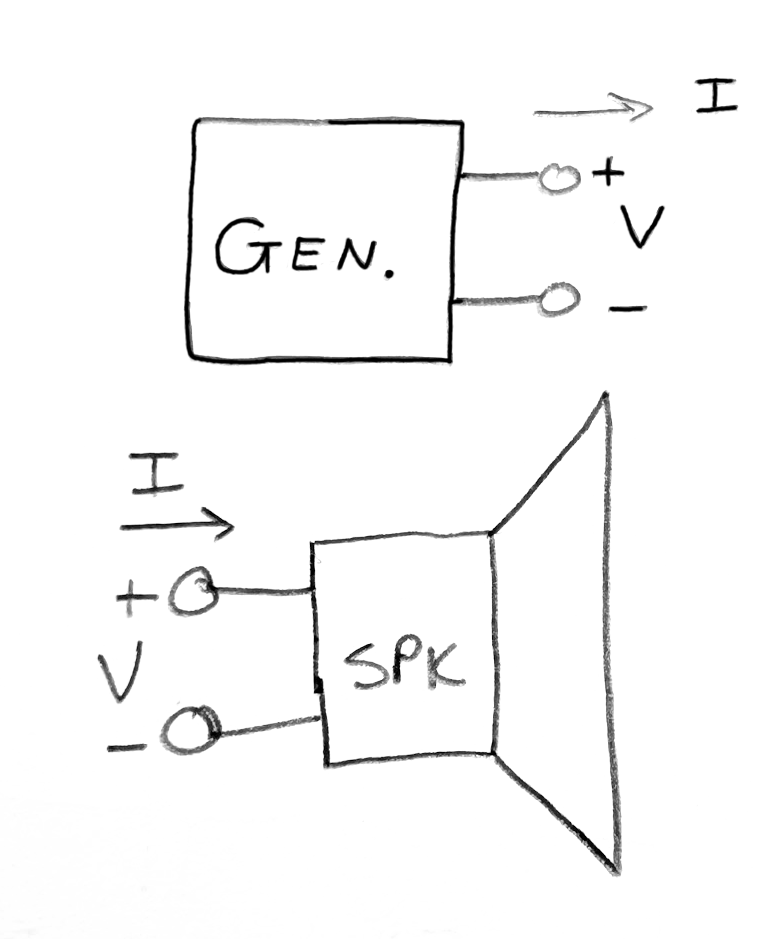
\includegraphics[width=0.3\textwidth]{figsChapt03/IE47318.png}

The $\pm$ indicates how we define positive voltage, and the direction arrow indicates
how we define positive current.

For the generator:
\[
P = VI = 1000V\times 10A = 10kW
\]
and for the speaker as shown:
\[
P = VI = 10V\times5A  =50W
\]
and everybody's happy.







\subsection{Power in the sinusoidal steady state}
Let's assume sinusoidal steady state and we have
\[
i(t) = I_M \cos(\omega t + \phi)
\]
\[
v(t) = V_M \cos(\omega t)
\]

\noindent We define the {\bf Average Power} as:
\[
P_{AV} = \frac{1}{T} \int_0^T i(t) v(t) \, dt
\]
where $T = \frac {\omega}  {2\pi}\;\; \text{the~period~of}  \;\; i(t), v(t) = \frac{2\pi}{\omega}$.


\noindent Note this is  also true of multiple periods,
\[
\int_0^{nT} dt \text{~~or~even} \int_{-\infty}^{-\infty}dt
\]



\noindent so,
\[
P_{AV_{\text{Sinusoid}}} = I_MV_M\frac{1}{T} \int_0^{2\pi/\omega}  \cos(\omega t + \phi) \cos(\omega t) dt
\]

\[
= I_M V_M \frac{\omega}{2\pi} \left[ \frac{\pi \cos(\phi)}{\omega} \right] \quad
\]
(We've looked up that integral in a table).   Finally we get:

\[
P_{AV_{\text{Sinusoid}}} = \frac{I_M V_M}{2} \cos(\phi)
\]
Where $ \phi = $ the angle between voltage and current.

Note that this is almost like the DC result, $P=IV$.   We
define the important quantity {\bf power factor}, as

\[
PF \equiv \cos(\phi)
\]
Power Factor is
a number between zero and 1 which depends on the phase angle between
voltage and current (note that PF is always positive for phase
angles between $\pm 90^\circ$.)


\subsection{Power in a General Impedance}

%\includegraphics[width=0.3\textwidth]{figsChapt03/SA65016.png}  %2-Oct-25
With reference to this simple circuit, we can write
%
% \[
% i(t) = I_M \cos(\omega t + \phi)
% \]
% \[
% \vec{V} = \vec{I} Z \Rightarrow v(t) = V_M \cos(\omega t + \phi + \angle z)
% \]
% \[
% (V_M = I_M |Z|)
% \]
% \[
% \alpha = \phi + \angle z
% \]

\[
p(t) = i(t) \cdot v(t)
\]
for the sinusoidal steady state, and defining $\phi=0$ according
to the phase angle of the applied voltage wave,
\[
v(t) = V_M\cos(\omega t)
\]
\[
i(t) = I_M\cos(\omega t + \phi)
\]
($V_M, I_M$ are real numbers)

\[
p(t) = v(t) \cdot i(t) = V_M I_M \cos(\omega t ) \cos(\omega t + \phi )
\]
(note that $\phi = \angle{Z}$)

\noindent A trig identity is the  product of cosines formula\footnote{See wikipedia trig indentities}:

\[
\cos(a) \cos(b) = \frac {1} {2} (\cos(a-b) + \cos(a+b))
\]
where $a=\omega t$ and $b=\omega t + \phi$.

So using that we get:

\[
p(t) = \frac{I_M V_M }{2} \cos(\omega t -\omega t - \phi) + \frac{I_M V_M}{2} \cos(\omega t + \omega t + \phi )
\]

\[
p(t) = \frac{I_M V_M }{2} \cos( \phi) + \frac{I_M V_M}{2} \cos(2\omega t + \phi )
\]
Note also that $\cos(-x) = \cos(x)$ and that $V$ and $I$ are related by
\[
\vec V = \vec I Z
\]
so $\phi = \angle {Z}$

Perhaps the  most useful form of the result is
\[
p(t) = \frac{I_M V_M }{2} \cos( \angle{Z}) + \frac{I_M V_M}{2} \cos(2\omega t + \angle{Z})
\]

This has two components.
{\bf 1)} The average power (a {\bf constant}, $\frac{V_M I_M}{2} \cos(\angle Z)$) and
{\bf 2)} a time varying power ($\frac{I_M V_M}{2} \cos(2\omega t   + \angle Z)$).

If we are using RMS values instead of the absolute magnitudes $V_M, I_M$,
we note
\[
\frac {V_MI_M}  {2} = |\vec V_R||\vec I_R| = V_R I_R
\]

so we also have
\[
p(t) = V_RI_R\cos(\angle{Z}) + V_RI_Rcos(2\omega+\angle{Z})
\]

\subsection{Computing Power Waveforms with Python}

\vspace{0.3in}
In the following, we will make some python computations of $v(t), p(t)$
with a fixed $i(t)$.   The color code will be:
\begin{center}
\begin{tabular}{l|l}\hline
black  &  Current \\
blue   &  Voltage \\
red    &  Instantaneous Power \\
\end{tabular}
\end{center}
The current will be the same in each case, e.g.
\[
i(t) = 1.0\cos(t) \;\; \text{Amps} \to  \vec I = 1.0 \angle 0^\circ
\]
The python code will simply compute $p(t)$ at each instant of time and plot it.

\begin{listing}
\begin{minted}{python}
import numpy as np
import matplotlib.pyplot as plt
#
#   Visualize sinusoidal voltage and current and power
#     for R, L, C
w = 1
C = 1
R = 2.0
L = 0.5
j = 0.0+1.0j

ZR = R
ZC = 1.0/(j*w*C)
ZL = j*w*L
# choose an element:
Z = ZC
# titlestr = 'Resistor'
titlestr = 'Capacitor'
# titlestr = 'Resistor'

phi = np.angle(Z)
T = np.linspace(0,5*np.pi/2, 50)
V = (1.0 + 0j) * np.e**(j*w*T)  # complex sinusoid voltage
I = V/Z
Vr = np.real(V)
Ir = np.real(I)
P = Vr*Ir
i=0
for t in T:
   print(t, Vr[i], Ir[i], P[i])
fig = plt.figure(figsize=(10,10))
ax = plt.gca()
data = [Ir, Vr, P]
colors=['k','b','r']
for i in range(3):
    plt.plot(T,data[i], color=colors[i])
pi = np.pi
tickpts = np.array(range(12))
tickvals = pi/4 * tickpts
ax.set_xticks(tickvals)
ax.set_xlabel('wt (rad)')
ax.set_ylabel('Amplitude')
ax.legend(['Current', 'Voltage', 'Inst. Pwr.'])
plt.title('Voltage, Current, Power: '+titlestr)
plt.grid()
plt.show()
\end{minted}
\caption{Python Code for visualizing power waveforms (red).}
\label{lst:basicTustin}
\end{listing}


\paragraph{Capacitor}
Consider a capacitor where
\[
Z = \frac{j}{\omega C}, \quad V_M = I_M |Z| = \frac{I_M}{\omega C}, \quad \angle z = -\pi/2
\]

and again we assume sinusoidal steady state with
\[
v(t) = V_M \cos(\omega t)
\]

\[
i(t) = I_M \cos(\omega t + \phi)
\]

then
\[
p(t) = \frac{I_M^2}{2\omega C} \cos(-\pi/2) + \frac{I_M^2}{2\omega C} \cos(2\omega t  - \frac{\pi}{2})
\]

\[
= \frac{I_M^2}{2\omega C} \sin(2\omega t  )
\]

Graphing this with python:

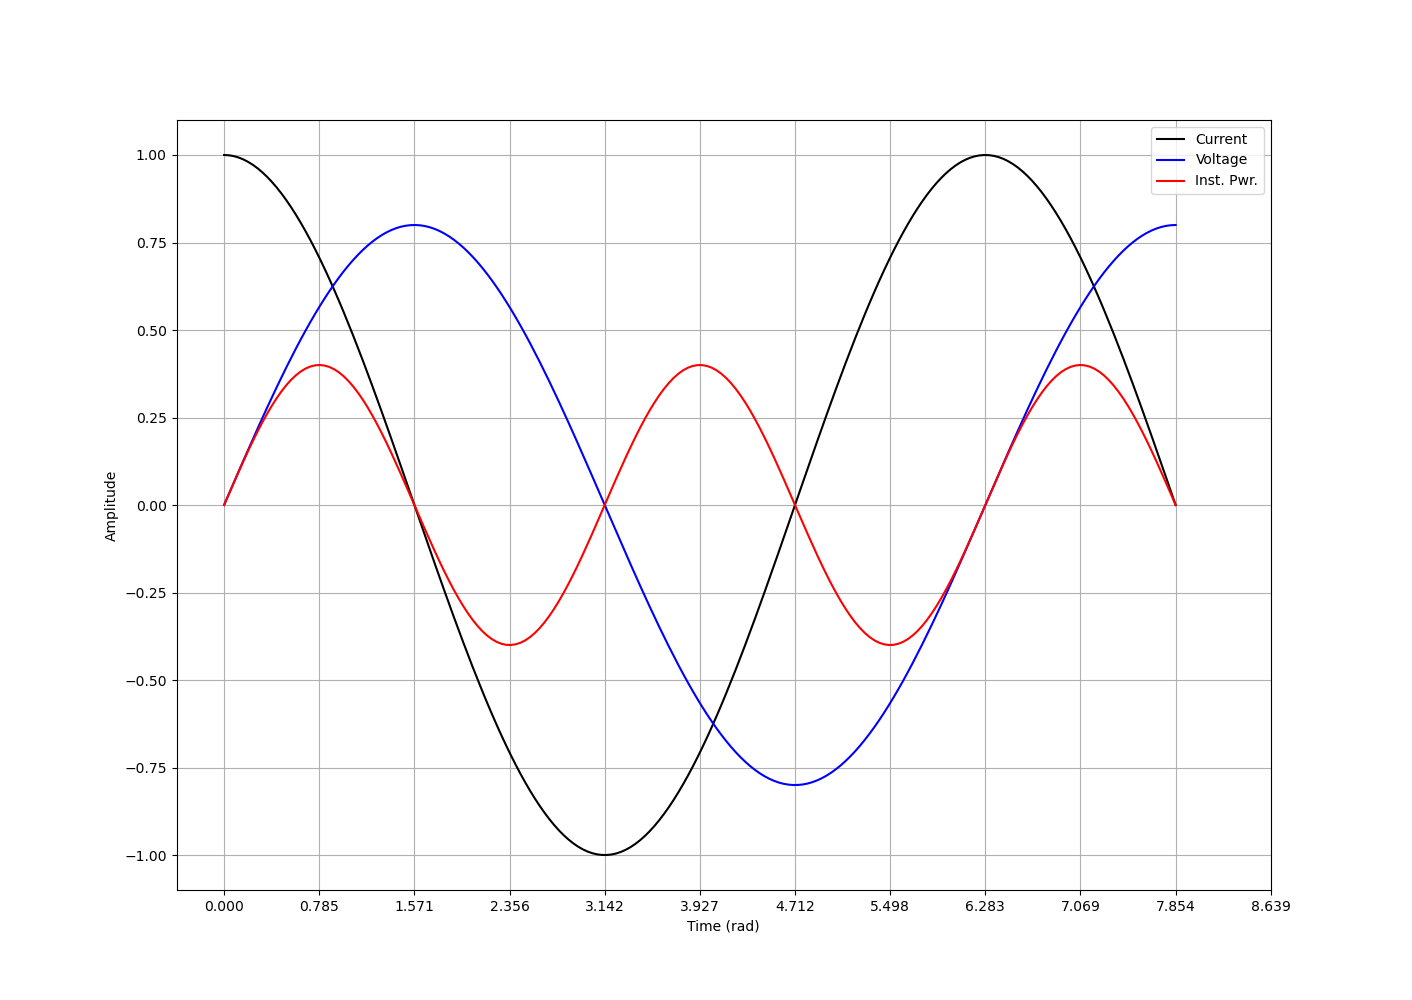
\includegraphics[width=0.5\textwidth]{figsChapt03/US73216.png}  %2-Oct-25

Observations:
\begin{enumerate}
    \item The frequency of power (red plot) is double the frequency of the voltage and current ($2\omega$).
    \item The power is   positive for the same amount of time as it is
    negative and has a smooth sinusoidal shape, so its average value
    (area under the wave divided by time), is zero.
    \item At a short time scale however power is alternating between
    positive and negative.  This means energy is alternately flowing
    into and out of the {\bf capacitor's electric field}.
\end{enumerate}

\subsection*{Resistor}

With a resistor of course voltage and current are related by
  $\vec V = \vec I R$ where $R$ is a real number.  Therefore the voltage and current sinusoids are perfectly in phase.
\[
Z = R \quad V_M = I_M R \quad \angle Z = \phi = 0
\]

\[
p(t) = \frac{I_M^2 R}{2} + \frac{I_M^2 R}{2} \cos(2\omega t + \phi)
\]
Observations:
\begin{enumerate}
    \item The frequency of power is double the freqency of the voltage and
    current ($2\omega$)
    \item The power is always positive at all times so its average value
    (area under the wave divided by time), is non-zero and positive.
\end{enumerate}

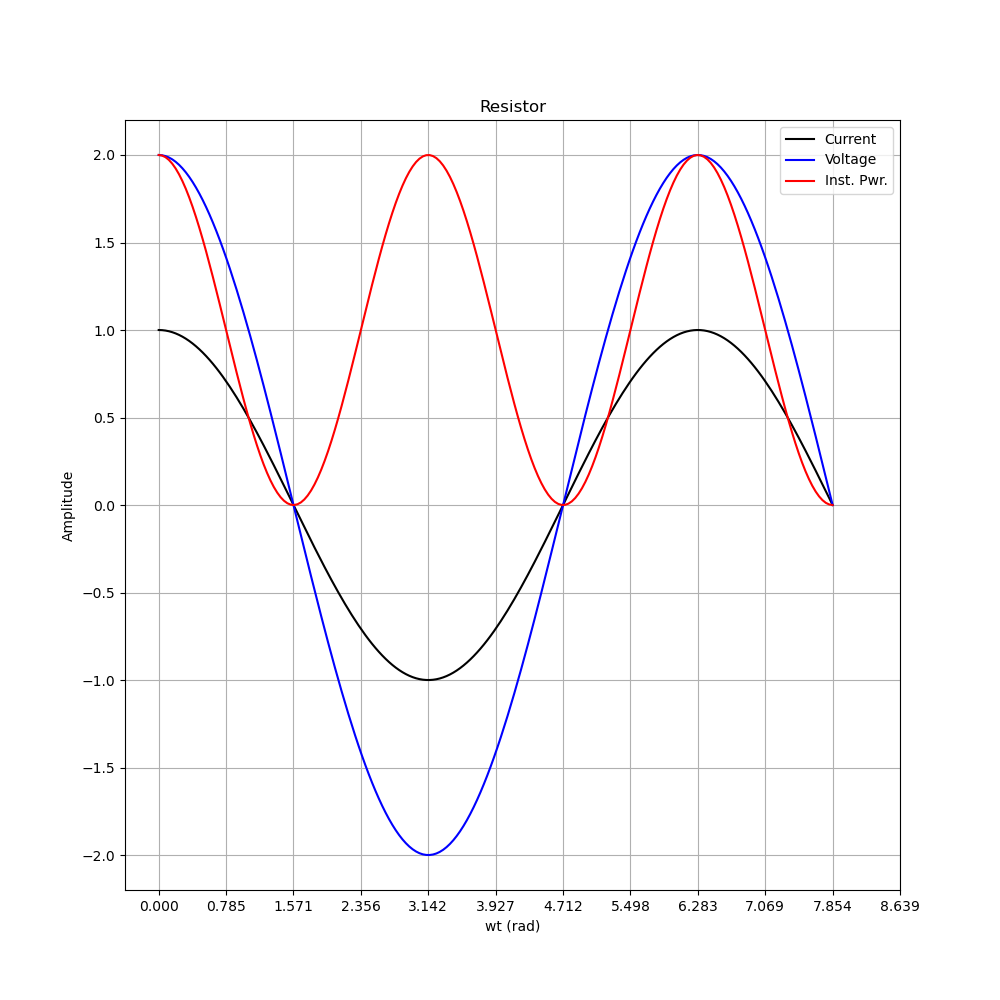
\includegraphics[width=0.5\textwidth]{figsChapt03/QI00215.png}

\subsection*{Inductor:}

Just as with the capacitor, the net power in an inductor is zero. (Note
different y-axis scale for this plot).
The phase shift is now $+\pi/2$ but the product of voltage and current
is still symmetrical about the $\omega t$ axis which averages to zero.

\[
Z = j\omega L \quad V_M = I_M \omega L \quad \angle z = \pi/2
\]

\[
p(t) = 0 + \frac{I_M^2}{2} \omega L \cos(2\omega t + 2\phi + \frac{\pi}{2})
\]

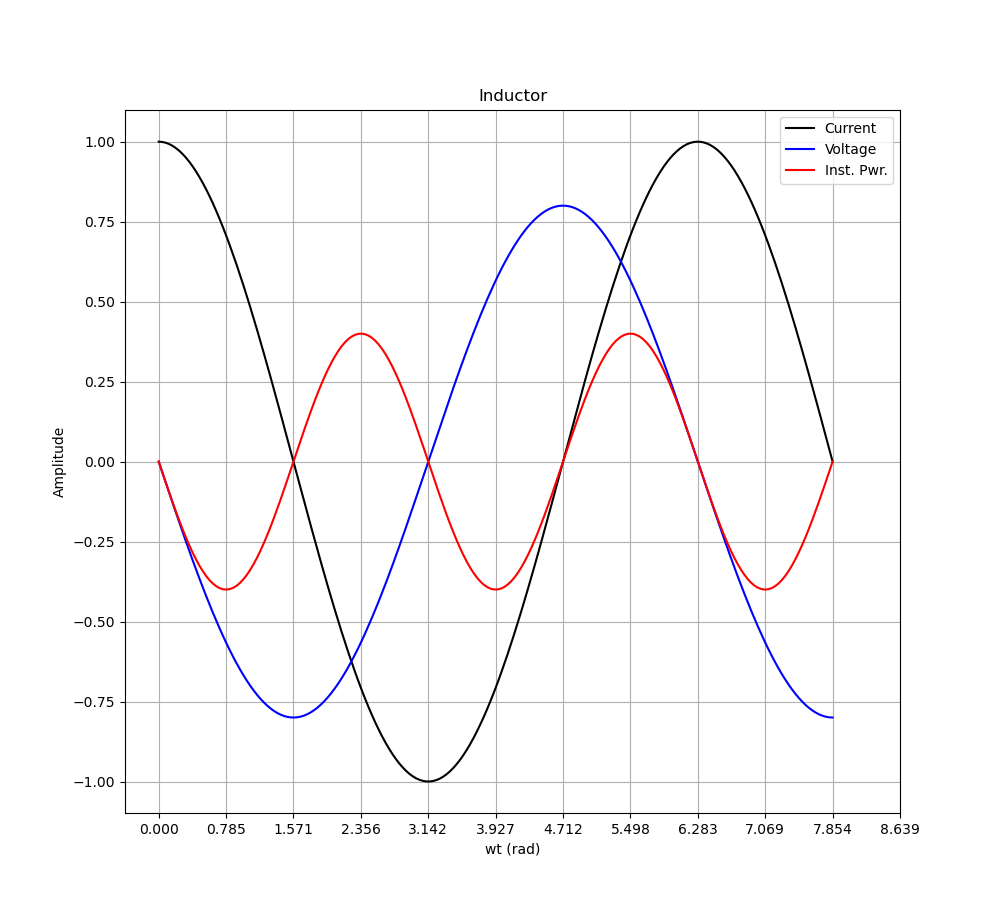
\includegraphics[width=0.5\textwidth]{figsChapt03/LN19448.png}


\begin{enumerate}
    \item The frequency of power (red plot) is double the frequency of the voltage and current ($2\omega$).
    \item The power is positive for the same amount of time as it is
    negative and has a smooth sinusoidal shape, so its average value
    (area under the wave divided by time), is zero.
    \item At a short time scale however power is alternating between
    positive and negative.  This means energy is alternately flowing
    into and out of the {\bf inductor's magnetic field}.
\end{enumerate}




\subsection*{Example:}


Find the average power sourced by the voltage source in this circuit:


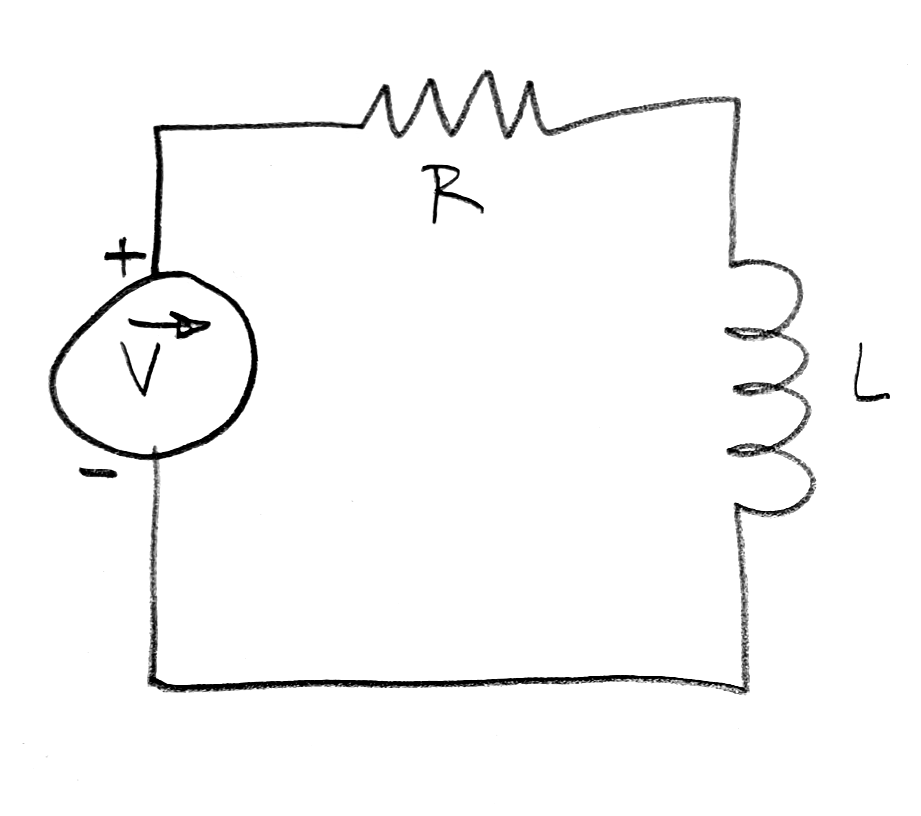
\includegraphics[width=0.4\textwidth]{figsChapt03/TU95372.png}


\[
\omega = 100 rad/s\;\; \vec{V} = 30 e^{j 0^\circ} = 30\; \mathrm{Volts}
\]

\[
R = 10 \Omega,\;\; L = 0.1 \text{H}
\]
\vspace{0.25in}
\noindent{\bf Solution:}


First, let's compute the impedance of the series circuit:
\[\boxed{
  Z = R+j\omega L = 10 + 10j = 7.07\angle 45^\circ
  }
\]


\noindent Since $\vec V$ is a sinusoid (with an absolute magnitude of
$V_M=30$), we can apply

\[
P_{AV} = \frac{I_M V_M}{2} \cos(\phi)
\]
where $\phi$ is the phase difference between voltage  and current.

\[
\vec{I} = \frac{\vec{V}}{Z},  \quad \phi = \angle{Z}
\]

putting $Z$ and $I$ in mag$\times$angle form:
\[
\vec{I} = \frac{\vec V}{Z} = \frac{30}{10\sqrt{2} e^{j45^\circ}} = I_M e^{j-45^\circ}
\]
\[\boxed{
    I_M=\frac{3}{\sqrt{2}}
  }
\]
\[
P_{AV} = \frac{I_M V_M}{2} \cos(\angle Z)
= \frac {3 \cdot 30}  {\sqrt{2}\cdot 2} \cos(-45^\circ)
\]
\[\boxed{
    P_{AV} = \frac {90}  {2\sqrt{2}}\cos(-\angle Z)  =  \frac {45}  {\sqrt{2}}\times 0.707 = 22.5\text{ Watts}
    }
\]


We call the factor $\cos(\angle Z)$ the {\bf power factor, PF}, a number
between 0 and 1 which determines how much average power we get from the
given voltage and current magnitudes.

Note that
\[
\mathrm{PF} = \cos\left(\tan^{-1}\left ( \frac {\mathrm{IM}\{Z\} }  {\mathrm{RE}\{Z\}}  \right ) \right) = \cos\left ( \angle{Z}\right )
\]


\vspace{0.3in}
Let's also
find $P_{AV}$ dissipated in just the resistor $R$ of the above circuit


\[
\vec I = \frac {3}  {\sqrt{2}} e^{j(-45^\circ)}
\]
converting to RMS:
\[
\vec {I}_R = \frac {1}  {\sqrt{2}} \vec I =  \frac {3}  {2} e^{j(-45^\circ)}
\]
Computing power in the resistor:
\[
P_R = \vec I_R \vec I_R^*\cdot R = |\vec I_R|^2R = \frac {9\cdot 10}  {4} = 22.5\text{ Watts}
\]


\noindent Note
\[
P_{AVR} = P_{AV_{\text{TOTAL}}}
\]
What we computed for the resistor alone is also the total for
the whole circuit because the inductor can dissipate no average power.

\newpage

\subsection{Summarizing: Power in AC elements}

\begin{tabular}{|c|c|c|c|c|c|}
\hline
Element & $Z$ & $\angle z$ & $pf$ & $p(t)$ & $\phi $ \\
\hline
R & $R + j0$ & 0 & 1 & $\frac{I_M^2 R}{2} + \frac{I_M^2 R}{2} \cos(\omega t)$ & \\
 & & & & $P_{AV}$ & $  0$ \\
\hline
L & $0 + j\omega L$ & $+90^\circ$ & 0 & $\frac{I_M^2}{2} \omega L \cos(2\omega t + \pi/2)$ & \\
 & & & & & $\pi/2$ \\
\hline
C & $0 - \frac{j}{\omega C}$ & $-90^\circ$ & 0 & $\frac{I_M^2}{2\omega C} \cos(2\omega t -\pi/2)$ & \\
 & & & & & $-\pi/2$ \\
\hline
Z & $R + jX$ & $\tan^{-1}(\frac{X}{R})$ & $\cos(\angle z)$ & & $ \angle z $ \\
\hline
\end{tabular}

\noindent Capacitors and Inductors (ideal ones) cannot dissipate power. Can only accumulate it and give it back. Only R element can dissipate Power.



\subsection{Optional Topic: Superposition of Power}

Here we will think about the question, ``Can we compute
two powers from two different sources separately and add them together?''

We'll check a simple example:

%
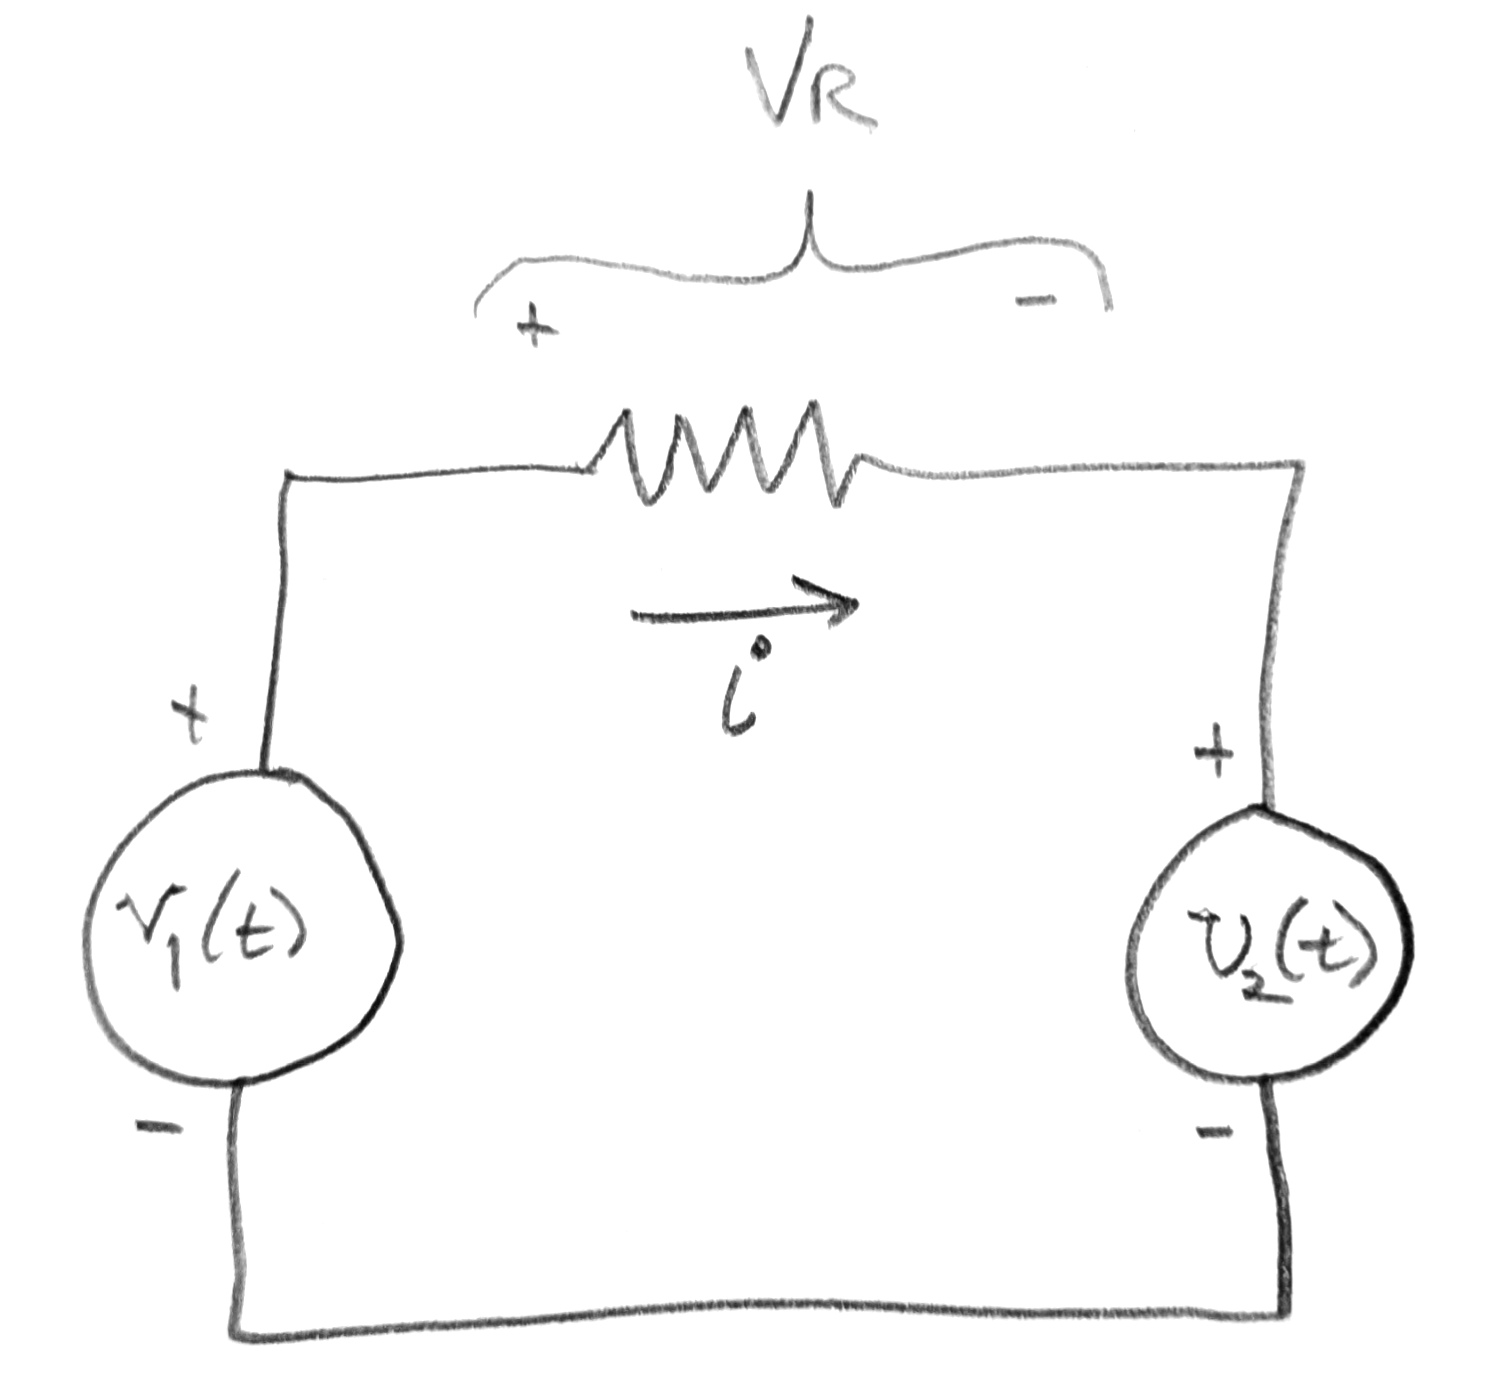
\includegraphics[width=0.4\textwidth]{figsChapt03/GP15083.png}



An approach based on superposition would say, let's set each
source to zero and compute the power delivered by the other source,
and then add them up, superimposing their solutions.
\[
i(t) = \frac{V_1(t)}{R} + \frac{V_2(t)}{R} = i_1(t) + i_2(t)
\]

using this sum to compute total power would give
\[
P(t) = i(t) V(t) \cdot R
= \left( i_1(t) + i_2(t) \right)^2 R
\]
\[
P(t) = \left( i_1^2(t) + i_2^2(t) \right) R + 2i_1(t) i_2(t) R
\]

But the last term means that we can't superpose power in this case at least.
But, suppose

\[
V_1(t) = V_1 \cos(\omega_1 t) \rightarrow i_1(t) = \frac{V_1 \cos(\omega_1 t)}{R}
\]

and
\[
V_2(t) = V_2 \cos(\omega_2 t) \rightarrow i_2(t) = \frac{V_2 \cos(\omega_2 t)}{R}
\]


where
\[
\omega_1 \neq \omega_2
\]

As we derived just above,
\[
P(t) = \frac{V_1^2 \cos^2(\omega_1 t)}{R} + \frac{V_2^2 \cos^2(\omega_2 t)}{R} + 2V_1 \cos(\omega_1 t) V_2 \cos(\omega_2 t) \frac{1}{R}
\]


We now need a new definition of average power because this $P(t)$ is not in general periodic.
For example, if $\frac{\omega_1}{\omega_2}$ is irrational, then the last term has no
exact period to integrate over.

We'll solve this for non-periodic signals  by

\[
P_{AV} = \lim_{\tau \rightarrow \infty} \frac{1}{\tau} \int_0^\tau p(t) \, d\tau
\]
(which of course also works for periodic
signals)

%continuing, we get
Taking this new average power of our superposition approach above, we get
\[
P_{AV} = \frac{1}{R} \lim_{\tau \rightarrow \infty} \frac{1}{\tau} \int_0^\tau \left[ V_1^2 \cos^2(\omega_1 t) + V_2^2 \cos^2(\omega_2 t) + 2V_1 \cos(\omega_1 t) V_2 \cos(\omega_2 t) \right] d\tau
\]
Let's call the three terms inside the integral (in brackets), $P_1, P_2, P_3$ in other words:
\[
P_{AV} =\frac{1}{R} \lim_{\tau \rightarrow \infty} \frac{1}{\tau} \int_0^\tau \left[
P_1 + P_2 + P_3 \right ] d\tau
\]

looking at $P_3$,  since $\omega_1 \neq \omega_2$,
\[
\frac{1}{R} \lim_{\tau \rightarrow \infty} \frac{1}{\tau} \int_0^\tau \left[ P_3 \right ] d\tau = 0
\]

\[
= P_{AV_1} + P_{AV_2} + \{ P_{12} = 0 \}
\]

The point is that if in the steady state sinusoidal case, if $\omega_1 \neq \omega_2$, we {\bf can} assume
superposition of power computation.

\subsection*{Significance of Superposition of power at different frequencies}

A circuit or system with input composed if many sinusoids can be analyzed w.r.t. avg power at each freq separately.  Examples of where we will use this include Audio, Communications,
and Control Systems.

 Conceptual Note: Voltages and currents of different frequencies are `orthogonal' in the sense that the power factor between them is zero.
 Thus no average power is dissipated in R by the product $v_1(t) v_2(t)$.

\noindent



\section{RMS Voltage and Current}
Recall: for sinusoids,
\[
P_{AV} = \frac{I_M V_M}{2} \cos(\phi)
\]

It is tempting to see this as a vector/dot product between voltage and current ($I_M V_M\angle \phi
$).

e.g.

\includegraphics[width=0.3\textwidth]{figsChapt03/UH48274.png}

But, what about factor of $\frac{1}{2}$?    To allow this dot-product interpretation of
voltage and current phasors, we need a new concept, the {\bf Root-Mean-Square, RMS} voltage
and current.

For any function $x(t)$,

\paragraph{Define}

\[
\text{RMS}(x(t)) = \sqrt{\frac{1}{T} \int_0^T (x(t))^2 \, dt}
\]
Note that this equation takes
\begin{enumerate}
    \item {\bf R: } The square root of ...
    \item {\bf M: }the mean $\left ( \frac{1}{T} \int_0^T ... ,\;\; dt \right )$ of ...
    \item {\bf S: }The square of $x(t)$
\end{enumerate}

If
\[
v(t) = V_M \cos(\omega t + \alpha)
\]

then
\[
\text{RMS}(v(t)) = \sqrt{\frac{\omega}{2\pi} \int_0^{2\pi/\omega} V_M^2 \cos^2(\omega t + \alpha) \, dt}
\]


\[
=\sqrt{ \frac{1}{2} V_M^2 }
= \frac{1}{\sqrt{2}} V_M \equiv V_{MR}
\]

(where $V_M, V_{NR}$ are real numbers).
We now can  define new phasors,
\[
\vec V_R = \frac {1}  {\sqrt{2}}  V_M e^{j\phi_1}
\]
\[
\vec I_R = \frac {1}  {\sqrt{2}}  I_M e^{j\phi_2}
\]

Since for sinusoids we are really just multiplying the magnitude by $\frac {1}  {\sqrt{2}} = 0.707$ it is useful to remember
that  the magnitude of the RMS phasor is just
\[
V_{MR} = 0.707 V_M
\]

\[
\vec V_R = 0.707 \vec V
\]

$V_{MR}$ is also the RMS value of the sinusoid in the time domain
which looks like:

\includegraphics[width=80mm]{figsChapt03/FP56580.png}


Similarly
\[
\text{RMS}(i_R) = \frac{1}{\sqrt{2}} I_M \equiv I_R
\]

\noindent Also note,

\[
V_R I_R \cos(\alpha - \phi) = \frac{V_M I_M}{2} \cos(\alpha - \phi)
\]

\[
= P_{AV}
\]



\noindent Now $P_{AV}$ corresponds to vector dot product

%\includegraphics[width=0.4\textwidth]{figsChapt03/phasor_rms.png}

\[
\vec{V}_R, \angle(\alpha)
\]

\[
\vec{I}_R \angle(\phi)
\]


\paragraph{Example:}  Consider
120 $V_{RMS}$, also known as North American Household voltage
\vspace{0.25in}
\noindent Q: what is $V(t)$?
\vspace{0.25in}

\noindent A:
\[
\frac{V_M}{\sqrt{2}} = V_{RMS}
\]

\[
V_M = \frac{ 120 } {0.707} = 170
\]

\[
V(t) = 170 \cos(377t)
\]

\includegraphics[width=0.5\textwidth]{figsChapt03/FM67804.png}



\subsection{RMS value of Non-Sinusoidal Pulse Train}
RMS value is not just for a sinuosoid.  It can be computed for any signal/waveform.
For example, let $V(t)$ be a train of rectangular pulses (between 0 and $A$ amplitude)
whose width can vary
independently of the period   as graphed below:


\includegraphics[width=0.5\textwidth]{figsChapt03/HT21139.png}


We call $\alpha $ the ``duty cycle'' \quad $0 \leq \alpha \leq 1$ which defines
how long the pulse lasts compared to the period, $T$.

\[
V_{RMS} = \sqrt{\frac{1}{T} \int_0^T V^2(t) \, dt}
\]

\[
= \sqrt{\frac{1}{T} \left[ \int_0^{\alpha T} A^2 \, dt +  \int_{\alpha T}^T 0^2 \, dt \right]}
= \sqrt{\frac{A^2}{T} [\int_0^{\alpha T} 1 \, dt] }
\]
\[
=\sqrt{\frac{A^2}{T} [ \alpha T] }= A\sqrt{\alpha}
\]

Note when
\[ \alpha = \frac{1}{2} \quad V_{RMS} = \frac{A}{\sqrt{2}}
\]
which is the same as a sinusoid for the amplitude.  But its mean is non-zero
compared to a zero-mean for a sinusoid.








\subsection{Additional Forms:  Power for Sinusoids}
With the RMS value, we now have

\[
P_{AV} = V_R I_R \cos(\angle z)
\]

\noindent Note also

if $Z = R + jX \rightarrow$

%\includegraphics[width=0.3\textwidth]{figsChapt03/impedance_diagram.png}

\[
\cos(\angle z) = \frac{R}{|Z|}
\]

\[
P_{AV} = \frac{V_R I_R}{\sqrt{2}} \frac{I_R}{\sqrt{2}} \cdot \frac{\text{Re}(Z^*)}{|Z|}
\]

\[
= \frac{I_R^2}{2} \text{Re}\{Z^*\}
\]

\[
P_{AV} = \frac{I_M^2}{2} \text{Re}\{Z^*\}
\]

So it is important to realize that  RMS Voltages and currents can
be viewed as analogous to
equivalent DC voltage/current such that
\[
P_{AV} = \vec I_R\times \vec V_R
\]


 We now have:

\[
P_{AV} = V_R I_R \cos(\angle z)
\]

  Note also that if

\[
Z = R + jX
\]

Like with any complex number,
\[
\cos(\angle Z) = \frac{R}{|Z|}
\]

Applying this to our average power result:
\[
P_{AV} = \frac{V_R I_R}{\sqrt{2}} \frac{I_M}{\sqrt{2}}  \frac{\mathrm{Re}\{Z\} }{|Z|}
\]
but
\[
\vec{I}_M = \frac{V_M}{Z}
\]

\[
= \frac{I_M^2}{2} \mathrm{Re}\left\{{Z}\right\}
\]



\subsection{RMS Phasors}   Using the RMS concept we can modify phasors to use
the RMS magnitude instead of absolute magnitude.

Take a voltage and current defined as

$i(t) = I_M \cos(\omega t + \phi)$

$v(t) = V_M \cos(\omega t + \phi + \angle z)$

Their phasors are
\[
\vec{I} = I_M e^{j\phi} \quad \vec{V} = V_M e^{j(\phi + \angle z)}
\]

\noindent Define ``RMS Phasor''

\[
\vec{I}_R = \frac{1}{\sqrt{2}} \vec{I} = \frac{I_M}{\sqrt{2}} e^{j\phi}, \quad \vec{V}_R = \frac{1}{\sqrt{2}} \vec{V} = \frac{V_M}{\sqrt{2}} e^{j(\phi + \angle z)}
\]

Let's multiply the RMS voltage phasor times the complex conjugate of the current
phasor ($\vec I_R^*$):

\[
\vec{V}_R \vec{I}_R^* = \frac{V_M I_M}{\sqrt{2}\sqrt{2}} e^{j(\phi + \angle z)} e^{-j\phi}
\]
(note how the CC changed the sign of $e^{-j\phi}$ exponent)

\[
= \frac{V_M I_M}{2} e^{j\angle z}
\]

Taking the real part of this complex number:
\[
\quad \text{Re}\{\vec{V}_R \vec{I}_R^*\} = \frac{V_M I_M}{2} \cos \angle z = P_{AV}
\]
Bottom line is we get the average power directly by multiplying RMS voltage phasor
times the complex conjugate of the current phasor.






\section{ ``Complex Power''}






We define a complex quantity
\[
S = P + jQ \equiv \vec{V}_R \vec{I}_R^*
\]
as the {\bf complex power} in a circuit.

For the RMS phasors:
\[
\vec V_R = V_Re^{j0},\;\vec I_R=I_Re^{j\phi}
\]
(we can assume the voltage phase is zero without loss of generality. Otherwise
$\phi = \theta_V - \theta_I$, and remember that $\phi = \angle{Z}$.)
The real and imaginary parts of $S$ are:
\[
P = \text{Re}\{\vec{V}_R \vec{I}_R^*\} = P_{AV} = V_R I_R \cos \angle Z
\]

\[
Q = \text{Im}\{\vec{V}_R \vec{I}_R^*\} = V_R I_R \sin \angle Z
\]

$P$ is the {\bf Real Power}

$Q$ is the {\bf Reactive Power}

Complex power can be plotted on the complex plane.  The Real Power, $P$, is
the real-axis component, and the Reactive Power, $jQ$ is the imaginary component
of Complex Power.

\vspace{0.25in}
\includegraphics[width=0.65\textwidth]{figsChapt03/A69D31.png}

Where $\theta = \angle{Z}$.

\subsection{Types of Power }
Summarizing the types of power so far!

\begin{center}
\begin{tabular}{|c|c|c|}
\hline
Type & Definition & Unit \\
\hline
Complex  & $S=P+jQ$   &  VA "Volt-Ampere"  \\
Real & $P_{AV}$, $\text{Re}\{S\}$, & Watts \\
 & $\frac{I_M^2}{2} \text{Re}\{Z\}$ etc. & \\
\hline
Reactive & $\text{Im}\{S\}$ & VAR ``Volt Ampere Reactive'' \\
 & $V_R I_R \sin \angle z$ etc. & \\
\hline
Apparent & $V_R I_R$ & VA ``Volt Ampere'' \\
\hline
\end{tabular}
\end{center}

Some facts obvious from the complex power diagram above:
\begin{enumerate}
\item Apparent Power $\geq$ Real Power
\item Apparent Power $\geq$ Reactive Power
\item Apparent Power $\leq$ Real Power + Reactive Power
\end{enumerate}








\subsection{Two Ways to get Complex Power in an Impedance}

\includegraphics[width=0.3\textwidth]{figsChapt03/MB87549.png}

1)
\[
 \quad S = \vec{V}_R \vec{I}_R^*,
\]
and,
\[
\vec{I}_R^* = \frac{\vec{V}_R^*}{Z^*}
\]

\begin{ExampleSmall}
Where we have used the following trick:

\noindent
Show that
\[
\left (\frac {a}  {b}\right )^*  =  \frac {a*}  {b*}
\]
where $a = ar+ja_i, b = br+jb_i$
\[
\left (\frac {a}  {b}\right )*  =  \left (\frac {ar+j a_i}  {br+jb_i} \right )^* =
\left (\frac {|a|}  {|b|} (\angle a - \angle b) \right )^*
\]
\[
= \left (\frac {|a|}  {|b|} (\angle b - \angle a) \right )
\]
\[
=\frac {|a|\angle b}  {|b|\angle a}
=\frac {|a|\angle -a}  {|b|\angle -b}
\]
showing that
\[
\left (\frac {a}  {b}\right )^*  =  \frac {a*}  {b*}
\]
\end{ExampleSmall}
\vspace{0.25in}

So
\[
S = \frac{\vec{V}_R \vec{V}_R^*}{Z^*} = \frac{|\vec{V}_R|^2}{Z^*}
\]
\[\boxed{
= \frac{V_M^2}{\vec{2}}\frac{1}{Z^*}
}
\]

2)
\[
\vec{V}_R = \vec{I}_R Z
\]

\[
S = \vec I_R \vec I_R^* Z
\]

\[
= |\vec{I}_R|^2 {Z} = I_R^2 {Z}
\]
\[
\boxed {
     S=  \frac{I_M^2}{2} {Z}
     }
\]

Notes:
\begin{itemize}
\item In both cases, $\angle S = \angle Z$

\item RMS current and voltage phasors can be used like DC voltage and current where

$R$, Resistance, $ \rightarrow Z$

$A^2$, Currrent squared, $ \rightarrow A A^* = |A|^2$
\end{itemize}

Summarizing:

\begin{center}
\begin{tabular}{c|c}
DC & RMS sinusoids \\
\hline
$P = I^2 R$ & $S = |\vec{I}_R|^2 Z$ \\
$P = \frac{V^2}{R}$ & $S = \frac{|\vec{V}_R|^2}{Z^*}$ \\
\end{tabular}
\end{center}





\subsection{Conservation of Complex Power}

\noindent Consider

\includegraphics[width=50mm]{figsChapt03/QM27615.png}

by KCL, (+ = leaving the node).   By $\vec V_R$ and $\vec I_R$ we mean
the RMS phasors for voltage and current.

\[
-\vec{I}_R + \vec{I}_{1} + \vec{I}_{2} = 0
\]


\[
\vec{I}_R = \vec{I}_{1} + \vec{I}_{2}
\]

\[
S = \vec{V} \vec{I}_R^* = \vec{V}_R (\vec{I}_{1}^* + \vec{I}_{2}^*)
\]

\[
= S_1 + S_2
\]

In other words, the power entering the circuit is the sum of the power in
$Z_1$ plus the power in $Z_2$.



\noindent Also consider the series circuit:

\includegraphics[width=80mm]{figsChapt03/RQ15238.png}

(where all quantities shown are RMS values.)
Using KVL:

\[
-\vec{V}_R + \vec{V}_{1R} + \vec{V}_{2R} = 0
\]

\[
 \vec{V}_R = V_{1R} + V_{2R}
\]

\[
S = \vec{V}_R \vec{I}_R^* = (\vec{V}_{1R} + \vec{V}_{2R}) \vec{I}_R^*
\]

\[
= S_1 + S_2
\]

Again, the complex power in whole circuit can be obtained by
adding complex power in each Z.  Which seems to agree with physical
intuition.




\subsection{Application: Power Factor Correction}

A power plant supplies electric power to a load over a long transmission line.
The transmission line has resistance, $R$.

\includegraphics[width=\textwidth]{figsChapt03/BN97423.png}


The power company collects revenue based on the average power delivered
to the customer (as that is what is measured by the electric meter, see below).


\[
P_{AV_{\text{user}}} = \text{Re}\{S_{\text{user}}\} \equiv  \$
\]

But the power plant sees an additional load which is dissipated in the
resistance of the transmission line.


\[
P_{\text{plant}} = \text{Re}\{S_{\text{user}}\} + |\vec{I}_R|^2 R
\]


The last term above is loss in the transmission line and the utility needs
 to minimize it because the user's meter does not see it.

Our user load is
\[
Z_L = R + jX
\]

Typically loads are more inductive, i.e. $X>0$.  Also we know that
\[
X>0,\;\; \theta = \angle Z_L > 0, \;\; \text{pf} < 1
\]

The user is paying for
\[
P_{AV_{\text{user}}} = \text{Re}\left\{ |\vec{I}_R|^2 Z_L \right\}
\]

\[
= \text{Re}\left\{ |\vec{I}_R|^2 |Z_L| (\cos \angle Z_L + j \sin \angle Z_L) \right\}
\]


\noindent Assume constant power use by the user, $P_{AV_{\text{user}}} = P$.
\[
P = |\vec{I}_R|^2 |Z_L| (\cos \theta)
\]

The wasted energy is the heating of the transmission line which is  $|\vec{I}_R|^2R$.
To reduce this waste, we can't change $R$,
so how does $\vec{I}_R$ depend on the power factor of $Z_L$?
From the previous result:

\[
|\vec{I}_R|^2 = \frac{P}{|Z_L| \cos \angle Z_L}
\]

Summing up, for fixed user power, $P$ and fixed $Z_L$, the power lost in
the transmission line, $|\vec{I}_R|^2 R$, is minimized (but not eliminated) when

\[
\cos \angle Z_L = 1
\]

So if the user can ``correct'' their power factor towards 1.0,
the utility saves money.
For this reason, utilities often are allowed to charge
an extra fee to users whose power factors fall below a  threshold (but the
threshold covers most regular houshold users. )

We move the power factor towards 1 by moving the
impedance angle to 0.
Looking at this graphically, suppose our power factor is too low because
the user's impedance ($Z_L$) has too much positive (inductive) reactance:

\vspace{0.15in}
\includegraphics[width=70mm]{figsChapt03/KM41864.png}

\[
Z_L = R + j\omega L
\]
\[
S = P + jQ_L
\]



Let's add a capacitor, $ C$  in parallel.

% ID44718
\vspace{0.1in}
\includegraphics[width=60mm]{figsChapt03/ID44718.png}
\vspace{0.1in}

We've seen that the total complex
power is the sum of that in each of the two parallel branches:

\[
S = S_C + S_{Z_L}
\]

The power in the capacitor is a pure reactive power:
\[
S_C = 0.0 + j Q_C
\]
we don't know its magnitude yet, only that it is pointing in the $-j$ direction
in the complex plane.   Lets suppose the inductive and capacitive reactances add
as shown below

\includegraphics[width=70mm]{figsChapt03/MF77903.png}

(i.e $|Q_C| < |Q_L|$)

Now we have a much smaller {\bf net} inductive reactance.   We have ``corrected''
the power factor of the load to a more acceptable level.

It can be shown that  if we want a desired power factor of $pf_d$ and that our phase
angle is therefore $\theta_{pfd} = \cos^{-1}(pf_d)$ that

\[
C = \frac{Q_L - P \tan \theta_{pfd}}{\sqrt{|\vec{VL}_R|^2} \omega}
\]
%
% were $VL_R$ is the RMS load voltage.
%
% % \hspace{4cm} look at pg 485
% %
% %
% % \noindent Problem 12.2.2
%
% %\includegraphics[width=0.5\textwidth]{figsChapt03/problem_circuit.png}
%
% \[
% < z_{TH}
% \]
%
% \[
% P_{AV_{\text{Source}}} = P_{AV_{AC}} + P_{AV_{DC}}
% \]
%
% by superposition of power
%
% at diff freq
%
% \[
% = \left\{ \text{Re}\{\vec{V}_{2R} \vec{I}_{2R}^*\} \right\} + \frac{2\pi}{T} \int_0^{2\pi/T} \left\{ 50 \cdot 0.1 \cos(1000t) \right\} dt
% \]
%
%
% \[
% = -\text{Re}\left\{ \vec{I}_{2R} Z_{TH} \vec{I}_{2R}^* \right\} + \frac{10}{1000} \int_0^{1000/2\pi} \left( \cos(1000)dt \right)
% \]
%
% \[
% = -\text{Re}\left\{ |\vec{I}_{2R}|^2 Z_{TH} \right\}
% \]
%
% \hspace{5cm} 0
%
% \[
% Z_{TH} = 500 \parallel -j1000 = 400 - 200j
% \]
%
% \[
% P_{AV_{\text{Source}}} = -\text{Re}\left\{ 0.005(400 + 200j) \right\}
% \]
%
% \[
% = -2 \text{ Watts }
% \]

%
% \noindent (Pages 8-10 appear to be magazine/newspaper clippings about power systems and the "Power plus" UW invention for boost delivery efficiency, not handwritten notes. I'll skip those.)


I asked {\tt Claude.ai} to help me find Seattle City light's official
rate for power factor charges.
\begin{quotation}
\noindent{\bf Official Rate Schedule}\\
Power Factor Charge: \$0.0015 per kVarh (kilovolt-ampere-reactive hour)\\
{\bf Conditions for Application}\\
The power factor penalty charge is only assessed if the power factor
is less than 97\%. Business Rates - City Light | seattle.gov
\end{quotation}
Note that a ``kVarh'' means reactive power of 1000 VAR for one hour,
or more formally:

\[
\text{kVarh} = \frac {1}  {1000}  \int_0^t Q(t) dt
\]
where $Q(t)$ is the reactive power as a function of time (such
as turning loads on and off), and t is measured in hours.


\subsection{Power Meters}

\begin{center}
\includegraphics[width=120mm]{figsChapt03/TS44996.png}
\end{center}


The traditional electric meter has two coils, the ``voltage coil'' in parallel
with the load, to sense voltage, and the ``current coil''
in series to sense current.   Together they drive a rotating disk at a rate proportional
to voltage times current.
The black dot indicates the correct polarity for a
positive power reading when power is absorbed by $Z_L$.


To the extent the meter is ideal, the impedances of the two coils are:
\[
Z_{cc} = 0
\]
\[
Z_{vc} = \infty
\]
so that they do not distort the measurement or consume much energy themselves.



The two coils drive a disk who's angular velocity is
proportional to real power.   Gears integrate the  velocity to the indicator dial
positions\footnote{Today a digital circuit might count revolutions and display
a number on an LCD instead.}.

When the load is wired according to the diagram with the correct polarity,

\[
V_{disk} \propto V_{LR} I_{LR} \cos \angle Z_L
\]



\begin{ExampleSmall}

\includegraphics[width=100mm]{figsChapt03/GD42554.png}

We model a power plant and distribution system as a phasor Thevenin equivalent
circuit (left), and then connect an ideal power meter between it and the load impedance $Z_2$
(right). \textbf{Question: What will meter read?}
\end{ExampleSmall}
\begin{ExampleCont}
\paragraph{Solution:} (using RMS phasors)
\[
\vec{I}_R = \frac{\vec{V}_R}{Z_1 + Z_2} \quad\quad\quad |\vec{I}_R| = \frac{|\vec{V}_R|}{| {Z}_1 +  {Z}_2|}
\]

Ignoring the ideal meter and using the voltage divider equation, we have

\hspace {1.75in} 1)
\[
\vec{V}_{2R} = \vec{I}_R Z_2 = \vec V_R \frac{Z_2}{(Z_1 + Z_2)}
\]


\[
S_{\text{Meter}} = \vec{I}_R\vec{V}_{2R}^*
\]
and also,

\[
P_{AV-Meter} = \mathrm{Re} \{S_{Meter}\} = |\vec I_R||\vec V_{2R}|\cos(\angle Z_2)
\]
We have


\hspace {1.75in} 2)
\[
\vec I_R = \frac {\vec V_{R}} {(Z_1+Z_2)}
\]
substituting,
\[
P_{AV-Meter} = \left |   \frac {\vec V_{R}}   {(Z_1+Z_2)}   \right |
\left | \vec V_R \frac{Z_2}{(Z_1 + Z_2)} \right | \cos(\angle Z_2)
\]
\[
= \frac{|\vec{V}_R| |\vec{V}_R| |Z_2|}
       {|(Z_1 + Z_2)|^2} \cos \angle Z_2
\]

\[\boxed{
P_{AV-Meter} = \frac{|\vec{V}_R|^2 |Z_2|}
                    {|(Z_1 + Z_2)|^2} \cos \angle Z_2
}
\]
(which will be the speed of the wheel inside the meter.)

\end{ExampleCont}











%
% 
\chapter{}

\section{}

\section{}

\section{}

\section{}

\section{}

\section{}

\section{}

\section{}

%
% % 
\chapter{}

\section{}

\section{}

\section{}

\section{}

\section{}

\section{}

\section{}

\section{}

% %
% 
\chapter{}

\section{}

\section{}

\section{}

\section{}

\section{}

\section{}

\section{}

\section{}

% %% Default Latex document template
%%
%%  blake@rcs.ee.washington.edu

\documentclass[letterpaper]{article}

% Uncomment for bibliog.
%\bibliographystyle{unsrt}

\usepackage{graphicx}
\usepackage{lineno}
%\usepackage{fancyhdr}

%%%%%%%%%%%%%%%%%%%%%%%%%%%%%%%%%%%%%%%%5
%
%  Set Up Margins

%%%%%%%%%%%%%%%%%%%%%%%%%%%%%%%%%%%%%%%%%%%%%%%%%
% include file for:
%      Critical Page setup dimensions
%            DO NOT MODIFY
%       (for help see "Latex Line by Line" p 260)
%
\setlength\oddsidemargin{0in}
\setlength\evensidemargin{0in}

\usepackage[left=0.98in, right=0.98in, top=1.0in, bottom=1.0in]{geometry}

% %Top Margin and header
% \setlength\voffset{-0.94in}
% \setlength\topmargin{0.25in}
% \setlength\headheight{0.25in}
% %\setlength\headwidth{6.5in}
% \setlength\headsep{0.25in}
% %Body
% \setlength\textwidth{6.5in}
% \setlength\textheight{9.50in}
% %Footer
% %\setlength\footheight{0.5in}
% \setlength\footskip{0.3750in}
% Line spacing for 6 lines per inch
\linespread{0.894}  % 1.0 = single    1.6 = double
%
%          END of Critical Page Setup Dimensions
%%%%%%%%%%%%%%%%%%%%%%%%%%%%%%%%%%%%%%%%%%%%%%%%%%%

%%%%%%%%%%%%%%%%%%%%%%%%%%%%%%%%%%%%%%%%%%%%%%%%%%%
%
% Useful style and math macros
%


\newcommand\Dfrac[2]{\frac{\displaystyle #1}{\displaystyle #2}}
\newcommand\beq{\begin{equation}}
\newcommand\eeq{\end{equation}}

\newcommand\bmat{\begin{bmatrix}}
\newcommand\emat{\end{bmatrix}}

\newenvironment{solution}
{\ttfamily \vspace{0.155in} {\bf SOLUTION:} \\ }
{ \vspace{0.25in} \par }



%
%        Font selection
%
%\renewcommand{\rmdefault}{ptm}             % Times
%\renewcommand{\rmdefault}{phv}             % Helvetica
%\renewcommand{\rmdefault}{pcr}             % Courier
%\renewcommand{\rmdefault}{pbk}             % Bookman
%\renewcommand{\rmdefault}{pag}             % Avant Garde
%\renewcommand{\rmdefault}{ppl}             % Palatino
%\renewcommand{\rmdefault}{pch}             % Charter


%%%%%%%%%%%%%%%%%%%%%%%%%%%%%%%%%%%%%%%%%%%%%%%%%
%
%         Page format Mods HERE
%
%Mod's to page size for this document
\addtolength\textwidth{0cm}
\addtolength\oddsidemargin{0cm}
\addtolength\headsep{0cm}
\addtolength\textheight{0cm}
%\linespread{0.894}   % 0.894 = 6 lines per inch, 1 = "single",  1.6 = "double"

% header options for fancyhdr

%\pagestyle{fancy}
%\lhead{LEFT HEADER}
%\chead{CENTER HEADER}
%\rhead{RIGHT HEADER}
%\lfoot{Hannaford, U. of Washington}
%\rfoot{\today}
%\cfoot{\thepage}



% Make table rows deeper
%\renewcommand\arraystretch{2.0}% Vertical Row size, 1.0 is for standard spacing)

\begin{document}
\setpagewiselinenumbers        %  Line numbers for edits to drafts.
\modulolinenumbers[1]          %  number every N lines

% \linenumbers                   %  start numbering lines here

\clearpage
\newpage
%%%%%%%%%%%%%%%%%%%%%%%%%%%%%%%%%%%%%%%%%%%%%%%%%%%%%%%%%%%%%%%%%%%%%%%%%%%%%%%%%%%%%%%%%%%%%%%%%%%%%%%%%%%%%%%%%%%%%%
\section{Complex Number Quiz}\label{ComplexNumberQuiz}
Take this quiz then check your answers on Page \pageref{CN_answers}.  Use only the following functions on your calculator (or fewer as instructed):

\[
* \quad \div + \quad - \quad \sqrt{x}
\]


It should be {\bf easy for you to get exact answers}.  If not, then you need to review the concepts in this quiz and section \ref{cnconcepts}.   Some Kahn Academy videos are pre-linked in Section \ref{KahnV}.


\begin{enumerate}

\item  What is $\sqrt{-16}$ ?

\item  Evaluate
\[
X = \frac{-b + \sqrt{4ac}}{2a}
\]
for the following values:
\begin{quotation}
\begin{tabular} {c|c|c}
a&b&c  \\ \hline
1&2&3 \\
1&-4&29\\
2&28&1156
\end{tabular}
\end{quotation}


\item  Evaluate
\[
(6+j16) + (-7-j6) =
\]
\[
(27-j0.75) - (1.6+j0.27) =
\]


\item  Evaluate  $M\times N$ where

\begin{quotation}
\begin{tabular} {c|c}
M&N \\ \hline
$(2+6j)$	&	$(1+3j)$   	\\
$(1.7-0.6j)$    &	$(3.2+0.4j)$	\\
\end{tabular}
\end{quotation}


\item  Plot the following points on the complex plane:
\[
a = -3+1.5j \qquad b = 2-j \qquad c = j
\]


\includegraphics[width=6cm]{figsapdx/00926a.png}



\item  Convert $X_1=(4+3j)$ to polar (magnitude-angle) form


\item  Convert $X_2=(-16+3.7j)$ to polar (magnitude-angle) form


\item  Represent $X_3 = (-1+6j)$ in exponential form

\item  For
\[
a = 3e^{j\pi/4} \qquad b = 2\angle{45^\circ}
\]
Convert them to ``$a+bj$'' form and multiply $a*b$ without using a calculator.

\end{enumerate}





%  Use name of bibliography files without .bib extension
%\bibliography{brl}
\end{document}








%%%%%%%%%%%%%%%%%%%%%%%%%%%%%%%%%%%%%%%%%%%%%%%%%%%%%%%%%%%%%%%%%%%%%%%%%%%%%%%%%%%%%%%%%%
\newpage
\chapter{Appendix}


%%%%%%%%%%%%%%%%%%%%%%%%%%%%%%%%%%%%%%%%%%%%%%%%%%%%%%%%%%%%%%%%%%%%%%%%%%%%%%%%%%%%%%%%%%%%%%%%%%%%%%%%%%%%%%%%%%%%%%
\section{Complex Number Quiz}\label{ComplexNumberQuiz}
Take this quiz then check your answers on Page \pageref{CN_answers}.  Use only the following functions on your calculator (or fewer as instructed):

\[
* \quad \div + \quad - \quad \sqrt{x}
\]


It should be {\bf easy for you to get exact answers}.  If not, then you need to review the concepts in this quiz and section \ref{cnconcepts}.   Some Kahn Academy videos are pre-linked in Section \ref{KahnV}.


\begin{enumerate}

\item  What is $\sqrt{-16}$ ?

\item  Evaluate
\[
X = \frac{-b + \sqrt{4ac}}{2a}
\]
for the following values:
\begin{quotation}
\begin{tabular} {c|c|c}
a&b&c  \\ \hline
1&2&3 \\
1&-4&29\\
2&28&1156
\end{tabular}
\end{quotation}


\item  Evaluate
\[
(6+j16) + (-7-j6) =
\]
\[
(27-j0.75) - (1.6+j0.27) =
\]


\item  Evaluate  $M\times N$ where

\begin{quotation}
\begin{tabular} {c|c}
M&N \\ \hline
$(2+6j)$	&	$(1+3j)$   	\\
$(1.7-0.6j)$    &	$(3.2+0.4j)$	\\
\end{tabular}
\end{quotation}


\item  Plot the following points on the complex plane:
\[
a = -3+1.5j \qquad b = 2-j \qquad c = j
\]


\includegraphics[width=6cm]{figsapdx/00926a.png}



\item  Convert $X_1=(4+3j)$ to polar (magnitude-angle) form


\item  Convert $X_2=(-16+3.7j)$ to polar (magnitude-angle) form


\item  Represent $X_3 = (-1+6j)$ in exponential form

\item  For
\[
a = 3e^{j\pi/4} \qquad b = 2\angle{45^\circ}
\]
Convert them to ``$a+bj$'' form and multiply $a*b$ without using a calculator.

\end{enumerate}




\clearpage
\newpage
\section{Complex Number Quiz Answers}\label{CN_answers}

\begin{enumerate}
\item 4j

\item $-1\pm j\sqrt{2} \qquad  2\pm j5 \qquad -7\pm j23  $

\item $-1+j10 \qquad 1.1-j1.02$

\item $-16+12j \qquad 5.68-1.24j$

\item graphing points $a,b,c$:

\includegraphics[width=6cm]{figsapdx/00927a.png}

\item $|X_1| = 5 \qquad \angle X_1 = \tan^{-1}(4/3) = 53.1^\circ$

\item $|X_2| = 16.42 \qquad \angle{X_2} = 167^\circ$

\item $X_3 = 6.08e^{j1.74}$ (note radians must be used in the exponential)

\item $|a| = 3, \; |b| = 2$,  $\angle a = 45^\circ,\; \angle b = 45^\circ$  by inspection.
\[
a = 3*0.707 + j3*0.707 = .2121+j.2121 \qquad b = 2*.707 + j2*.707 = .1414+j.1414
\]
using {\it angles add, magnitudes multiply}, $a*b = 3*2e^{j\frac{\pi}{2}} = 6e^j = 6j$

\end{enumerate}


%%%%%%%%%%%%%%%%%%%%%%%%%%%%%%%%%%%%%

\section{Log Quiz Answers}\label{Log_answers}


\begin{enumerate}

\item $\log(A) + \log(B)$

\item $2\log(a)+\frac{\log(b)}{2}$

\item $6-\log(R)$

\item $27.4$

\item $27.4/\ln(10)$

\end{enumerate}



\end{document}
